\documentclass[10pt,a4paper,oneside]{ctexbook}
\usepackage{geometry}
\geometry{margin=2.5cm}

% 数学、表格相关宏包
\usepackage{amsmath,amssymb}
\usepackage{array,caption,booktabs}
% 列表全局缩进设置
\usepackage{enumitem}
\setlist{leftmargin=2em}

% 绘图、电路、封面背景图依赖
\usepackage{graphicx}
\usepackage{tikz}
\usepackage{circuitikz}
\usetikzlibrary{circuits.logic.US,circuits.logic.IEC}
% 格式化网址链接，封面GitHub地址专用
\usepackage{url}

% hyperref 必须放在所有宏包最后
\usepackage{hyperref}
\hypersetup{
    colorlinks=true,
    linkcolor=black,
    filecolor=black,
    urlcolor=black,
    citecolor=black,
    pdfborder={0 0 0}
}

\begin{document}
% 封面
\begin{titlepage}
    \centering
    % 顶部间距调整，布局更均衡
    \vspace*{3cm}
    
    % 主标题
    {\Huge \bfseries 数字电子技术基础课程笔记 \par}
    \vspace{1.5cm}
    
    % 副标题
    {\Large 数制与码制、逻辑代数基础 \par}
    \vspace{2cm}
    
    % 贴合数电主题的名言
    {\itshape \large “数字电路的世界里，0和1构成了所有逻辑的基石。” \par}
    {\large —— 克劳德·香农（Claude Elwood Shannon） \par}
    \vspace{2.5cm}
    
    % 作者信息（完全复用指定内容）
    {\Large 作者：浮萍 \par}
    \vspace{0.5cm}
    
    % 版本号
    {\large 版本：1.0 完整版 \par}
    \vspace{0.5cm}
    
    % 联系方式（完全复用指定内容）
    {\large 邮箱：3071974740@qq.com \par}
    \vspace{0.5cm}
    
    % GitHub链接（完全复用指定内容）
    {\large GitHub：https://github.com/Duckweed-yhb \par}
    \vspace{1cm}
    
    % 生成日期
    {\large \today \par}
\end{titlepage}
\clearpage

% 目录
\tableofcontents
\clearpage

% 分章节笔记文件
\chapter{绪论}
\setlength{\parskip}{0.4em}
\setlength{\itemsep}{0.2em}
\setlength{\tabcolsep}{4pt}

\section{数字信号与数字电路}
\subsection{模拟量与数字量}
自然界的物理量就其变化规律而言不外乎两大类。

\begin{itemize}
    \item \textbf{模拟量}：在时间上或数量上的变化是连续的。如加热炉内的温度、水库水位的高度，相邻两值之间总可插入无穷多个中间值。
    \item \textbf{数字量}：在时间上和数量上都是离散的，变化发生在不连续的瞬间，且数值的大小与每次的增减都是某个\textbf{最小数量单位} $\Delta$ 的整数倍。如统计每天从装配线上输出的汽车数量。
\end{itemize}

把模拟量、数字量转换成电压（或电流）信号，得到的信号也分为两大类：\textbf{模拟信号}表征模拟量，幅值随时间连续变化；\textbf{数字信号}表征数字量，只取有限个离散状态，在二进制数字电路中仅取高、低两种电平，用 $1$、$0$ 表示。工作在模拟信号下的电子电路称为\textbf{模拟电路}，工作在数字信号下的电子电路称为\textbf{数字电路}。

需要强调：数字信号中的 ``$1$'' 和 ``$0$'' \textbf{没有数量的意义}，只表示事物的两个对立面（高/低电平、开关通/断、灯亮/灭），其数量含义要由\textbf{数制}和\textbf{码制}另行赋予。

\subsection{数字电路与模拟电路的比较}
二者在工作信号、研究对象、分析设计方法以及所用的数学工具上都有明显不同，见表~\ref{tab:dig_vs_ana}。

\begin{table}[!htbp]
    \centering
    \caption{数字电路与模拟电路的比较}
    \label{tab:dig_vs_ana}
    \begin{tabular}{@{}lll@{}}
        \toprule
        对比维度 & 数字电路 & 模拟电路 \\
        \midrule
        工作信号 & 离散的高、低电平序列 & 连续的电压、电流波形 \\
        取值特点 & 只有 $0$、$1$ 两种状态，可容偏差 & 连续取值，精度依赖器件一致性 \\
        研究对象 & 输入输出的逻辑关系与时序关系 & 信号的放大、变换与波形质量 \\
        分析方法 & 逻辑代数、真值表、卡诺图、状态转换 & KCL/KVL、小信号等效电路、频响分析 \\
        数学工具 & 离散数学（布尔代数） & 微积分、复变函数、线性代数 \\
        \bottomrule
    \end{tabular}
\end{table}

\subsection{数字电路的主要优点}
\begin{enumerate}
    \item \textbf{抗干扰、容偏差}：每一位只有 $0$、$1$ 两种取值，电路只要能正确区分两种状态即可，无须精确复制某个电压值，因而对制造精度、工作条件和运行环境的要求大大降低。
    \item \textbf{精度可扩展}：需要提高精度时只需增加二进制数的位数，不必提高单个器件的精度。
    \item \textbf{便于集成与存储}：单元电路重复性强，易于大规模集成；信息以代码形式保存，便于长期存储与复制。
\end{enumerate}
正因为对制造精度要求相对宽松，\textbf{首先制成的集成电路是数字集成电路}；迄今为止大多数大规模、超大规模集成电路都属于数字集成电路。

为充分发挥数字电路在信号处理上的优势，可先将模拟信号按比例转换成数字信号，送入数字电路（或计算机）处理，再把结果转换成模拟信号输出。自 20 世纪 70 年代以来，这种用数字电路处理模拟信号的``数字化''浪潮已席卷几乎所有电子技术应用领域。

\section{电子技术的发展历程}
电子技术的发展与进步，是与电子器件的更新紧密相连的。表~\ref{tab:dev_history} 按代表性器件给出四个阶段的划分。

\begin{table}[!htbp]
    \centering
    \caption{电子技术发展的四个阶段}
    \label{tab:dev_history}
    \begin{tabular}{@{}llll@{}}
        \toprule
        阶段 & 年代 & 代表器件 & 主要特征与应用 \\
        \midrule
        第一阶段 & 20 世纪 40 年代 & 电子管（真空管） & 早期计算机、电话交换、数字通信 \\
        第二阶段 & 20 世纪 60 年代 & 晶体管（半导体三极管） & 功耗小、寿命长、体积小，扩展到测量领域 \\
        第三阶段 & 20 世纪 70 年代中期 & 集成电路（IC） & 数字技术广泛应用，进入医疗、雷达、卫星 \\
        第四阶段 & 70 年代中至 80 年代中 & 大规模、超大规模 IC & 微电子技术迅猛发展，渗透到各行各业 \\
        \bottomrule
    \end{tabular}
\end{table}

\subsection{关键器件与事件}
\begin{itemize}
    \item \textbf{1904 年，真空二极管}：19 世纪 80 年代爱迪生发现``爱迪生效应''，弗莱明据此发明真空二极管；德福雷斯特在灯丝与板极之间加入栅极，发明第一只真空三极管，被看作电子工业真正的诞生起点。电子管工作时须将阴极加热到很高温度，因而功耗大、寿命短、体积重量大、噪声大、工艺复杂。
    \item \textbf{1947 年，晶体管}：布拉顿（W. Brattain）、巴丁（J. Bardeen）和肖克利（W. Shockley）发明半导体三极管，功耗小、寿命长、体积重量大大减小，几乎在所有领域逐步取代电子管，发明者获诺贝尔奖。
    \item \textbf{1958 年，集成电路}：基尔比（J. Kilby）将若干晶体管、电阻及连线制作在一小片硅片上；同一时期诺伊斯（R. Noyce，Fairchild）也独立实现了集成电路，开辟了电子电路微型化的新途径。
    \item \textbf{1965 年，摩尔定律}：摩尔（G. E. Moore）提出集成电路中晶体管数目将以每年翻一番的速度增长（20 世纪 80 年代末以后翻番时间放慢到约 18 个月），同时每个晶体管的价格降为原来的一半。这一预测被实践所证明，称为``摩尔定律''。
    \item \textbf{当代}：已能把上亿个晶体管集成在一片邮票大小的硅片上，甚至把整个系统集成为``片上系统''（System on Chip，SoC）。2010 年集成电路微细加工精度已达 32\,nm；集成度的提高最终受加工工艺极限与晶体管物理极限的限制，摩尔定律也终将失效。
\end{itemize}

\subsection{电子电路的核心功能}
电子电路的功能可统一概括为\textbf{信息处理}与\textbf{能量转换}：模拟电路用连续的模拟电压、电流值表示信息；数字电路用一个离散的电压序列（$0/1$ 代码序列）表示信息。

\section{数字电路的特点与分类}
\subsection{数字电路的特点}
\begin{enumerate}
    \item \textbf{开关工作}：半导体器件工作在开关状态（截止或饱和/导通），只区分高、低两种电平。
    \item \textbf{二值描述}：输入、输出量都可用二值逻辑变量表示，输入与输出之间是逻辑上的因果关系，可用逻辑函数 $Y=F(A,B,C,\cdots)$ 描述。
    \item \textbf{研究重点}：不追求波形保真，而关心逻辑关系是否正确、时序是否满足要求、电平是否符合接口规范。
\end{enumerate}

\subsection{分类}
\begin{itemize}
    \item 按处理的信号形式：模拟电路、数字电路。
    \item 按输出与历史状态是否有关：\textbf{组合逻辑电路}（输出仅取决于该时刻输入）与\textbf{时序逻辑电路}（输出还与电路原状态有关）。
    \item 按所用器件：\textbf{双极型}（TTL、ECL 等）与\textbf{单极型}（CMOS 等）。
    \item 按集成度：\textbf{小规模}（SSI，基本门、触发器）、\textbf{中规模}（MSI，译码器、数据选择器、计数器）、\textbf{大规模}（LSI，存储器、可编程逻辑器件）、\textbf{超大规模}（VLSI，CPU、SoC）。
    \item 按层级：单体 MOSFET $\rightarrow$ 逻辑门 $\rightarrow$ 组合/时序功能块 $\rightarrow$ 复杂数字系统。
\end{itemize}

\section{可编程逻辑器件与 EDA 技术}
\subsection{从固定逻辑到可编程逻辑}
早期数字集成电路的逻辑功能在制造时即已固定，要改变功能就必须改变内部单元电路之间的连接，而连接在制作过程中已经固定下来。若制作一种允许用户自行修改内部连接的通用集成电路，则只需生产这一种器件就能满足不同用户的需要，这种器件称为\textbf{可编程逻辑器件}（Programmable Logic Device，\textbf{PLD}）。PLD 的内部电路结构可通过写入编程数据来设置，部分器件的编程数据还可擦除重写。PLD 最初出现在 20 世纪 60 年代后期，80 年代以后获得迅猛发展。

需要注意：微处理器和单片机也是可编程的大规模数字集成电路，但对它们编程并不改变电路的内部连接结构，只是写入运行程序，其内容属于``微机原理''等后续课程。

\subsection{EDA 技术}
如此复杂的编程工作无法用手工完成，PLD 的编程（包括编程数据的生成和写入）必须使用 \textbf{EDA}（Electronics Design Automation，电子设计自动化）技术。其工具包含硬件和软件两部分：
\begin{itemize}
    \item \textbf{硬件}：计算机和编程器；
    \item \textbf{软件}：用于描述电路功能的\textbf{硬件描述语言}（Hardware Description Language，\textbf{HDL}）及其编译程序，以及适应于选用器件的编程软件，用以完成编程数据的生成与写入。
\end{itemize}

早期 PLD 需先把计算机生成的编程数据输入编程器，再写入置于编程器上的器件；如今大规模集成的 PLD 越来越多地采用``\textbf{在系统可编程}''（In System Programmable，\textbf{ISP}）技术，编程数据可直接写入已安装在系统里的器件，无须专用编程器，也不必把器件从系统中取出。

本课程涉及的现代设计流程可概括为：逻辑功能描述（HDL）$\rightarrow$ 逻辑综合 $\rightarrow$ 仿真验证 $\rightarrow$ 布局布线 $\rightarrow$ 下载/编程 $\rightarrow$ 硬件测试。

\section{课程内容与学习方法}
\subsection{课程体系中的位置}
先修\textbf{电路原理}；平行\textbf{模拟电子技术基础}及其实验、\textbf{数字电子技术基础}及其实验；后续\textbf{微机原理}、\textbf{嵌入式系统}。

\subsection{课程目的与基本要求}
课程目的是掌握\textbf{基本概念、基本分析方法、基本设计方法和基本实验技能}，可分解为四项核心能力：
\begin{enumerate}
    \item 基础概念：逻辑电平、逻辑门、组合/时序、噪声容限等；
    \item 电路分析方法：由电路求逻辑功能、由波形求真值表、时序分析；
    \item 电路设计方法：由功能要求选器件、化简、画逻辑图、验证；
    \item 实验技能：仪器使用、电路搭接与调试、故障定位。
\end{enumerate}

\subsection{学习方法}
\begin{itemize}
    \item \textbf{自底向上（Bottom-up）}：先理解器件与门如何工作，再逐级抽象到功能块与系统。
    \item \textbf{抓抽象与接口}：抽象方法与接口约定是复杂系统可管理的关键；接口应具备良好的隔离特性以及扩展、升级特性。
    \item \textbf{分层训练}：在各层级上掌握设计电路的方法，兼顾学科历史、系统方法、算法与电路调试方法。
    \item \textbf{重实践}：逻辑代数与化简必须动手推导，门电路与时序电路必须结合波形和实验现象理解。
\end{itemize}

优质数字系统设计的准则：结构化设计，每一级保持有限的复杂度，支持模块复用；以最小的代价实现最大的功能，实现可靠的系统，并保持对未来技术的兼容性。

\clearpage

% 数制和码制 子文件，匹配PPT章节顺序，无手动编号，无冗余应试文字
\chapter{数制和码制}
\section{概述}
\begin{enumerate}
    \item 数制：带位权的进位计数规则；码制：信息向二进制映射的编码规则。
    \item 数字信号仅用0、1表征两种对立电平/开关状态，依靠数制、码制赋予数值与字符含义。
\end{enumerate}

\section{几种常用的数制}
\subsection{通用定义与位权展开公式}
基数$N$：数制内可用数码总个数；位权：$N^i$；任意$n$位整数、$m$位小数的$N$进制数展开：
\[
(X)_N=\sum_{i=-m}^{n-1}k_i \cdot N^i,\quad 0\le k_i\le N-1
\]
\begin{itemize}
    \item 十进制D：基数10，逢十进一，数码0~9，位权$10^i$
    \item 二进制B：基数2，逢二进一，数码0/1，数字电路基础，位权$2^i$
    \item 八进制O：基数8，逢八进一，数码0~7，位权$8^i$
    \item 十六进制H：基数16，逢十六进一，数码0~9、A(10)~F(15)，位权$16^i$
\end{itemize}

\subsection{0~15多进制对照表}
\begin{table}[!htbp]
    \centering
    \setlength{\tabcolsep}{10pt}
    \renewcommand{\arraystretch}{1.3}
    \caption{0~15十进制、二进制、八进制、十六进制对应关系}
    \label{tab:num_0_15}
    \begin{tabular}{|c|c|c|c|c|c|c|c|}
        \hline
        D & B & O & H & D & B & O & H \\
        \hline
        0  & 0000 & 00 & 0 & 8  & 1000 & 10 & 8 \\
        1  & 0001 & 01 & 1 & 9  & 1001 & 11 & 9 \\
        2  & 0010 & 02 & 2 & 10 & 1010 & 12 & A \\
        3  & 0011 & 03 & 3 & 11 & 1011 & 13 & B \\
        4  & 0100 & 04 & 4 & 12 & 1100 & 14 & C \\
        5  & 0101 & 05 & 5 & 13 & 1101 & 15 & D \\
        6  & 0110 & 06 & 6 & 14 & 1110 & 16 & E \\
        7  & 0111 & 07 & 7 & 15 & 1111 & 17 & F \\
        \hline
    \end{tabular}
\end{table}

\section{不同数制间的转换}
\subsection{任意进制转十进制}
方法：按位权展开求和，核心公式：
\[
(X)_N=\sum_{i=-m}^{n-1}k_i N^i
\]

\subsection{十进制转N进制}
\begin{itemize}
    \item 整数部分：\textbf{除N取余，逆序排列}，直至商为0
    \item 小数部分：\textbf{乘N取整，顺序排列}，至小数为0或满足精度
    \item 特例：转二进制替换基数为2；转八/十六进制同理替换基数
\end{itemize}

\subsection{二进制与八/十六进制互转}
\begin{table}[!htbp]
    \centering
    \setlength{\tabcolsep}{12pt}
    \renewcommand{\arraystretch}{1.3}
    \caption{分组转换规则}
    \label{tab:bin_group_rule}
    \begin{tabular}{|c|c|}
        \hline
        转换方向 & 操作步骤 \\
        \hline
        B $\to$ O & 小数点向两侧每3位分组，不足补0，每组对应1位八进制 \\
        B $\to$ H & 小数点向两侧每4位分组，不足补0，每组对应1位十六进制 \\
        O $\to$ B & 1位八进制展开为3位二进制，删除首尾多余前导0 \\
        H $\to$ B & 1位十六进制展开为4位二进制，删除首尾多余前导0 \\
        \hline
    \end{tabular}
\end{table}

\section{二进制算数运算}
\subsection{基础四则运算规则}
二进制加减乘除遵循：逢二进一、借一当二；乘法/除法可拆解为移位+加法，减法统一转化为\textbf{加补码}。

\subsection{原码、反码、补码}
带符号二进制数由符号位+数值位构成：最高位为符号位，0表示正数，1表示负数，剩余低位为数值位。
\subsubsection{原码}
定义：符号位加上数值绝对值对应的二进制码。
\begin{itemize}
    \item 正数原码：符号位为0，数值位等于真值；
    \item 负数原码：符号位为1，数值位等于真值绝对值；
    \item 特性：数字0存在两种编码，$[+0]_{\text{原}}$、$[-0]_{\text{原}}$，不便于减法运算。
    \item 用途：二进制负数直观表示，仅用于人工阅读，硬件不做运算。
\end{itemize}

\subsubsection{反码}
定义：基于原码按位取反得到。
\begin{itemize}
    \item 正数反码：与自身原码完全相等；
    \item 负数反码：符号位保持1不变，数值位全部按位取反（0变1，1变0）；
    \item 特性：数字0仍存在两种编码，不能统一0的表示。
    \item 用途：原码转换补码的中间过渡编码，无独立运算价值。
\end{itemize}

\subsubsection{补码}
定义：计算机系统实际存储、运算使用的编码，消除0的二义性，实现减法转加法。
\begin{itemize}
    \item 正数补码：补码 = 原码 = 反码；
    \item 负数补码：对负数的反码加1；
    \item $n$位带符号补码取值范围：$\boldsymbol{-2^{n-1} \le X \le 2^{n-1}-1}$；
    \item 特性：数字0仅有唯一补码表示；符号位可直接参与加法运算。
    \item 运算核心公式：$[A-B]_{\text{补}} = [A]_{\text{补}} + [-B]_{\text{补}}$；
    \item 溢出规则：加法产生最高进位直接舍弃；运算结果超出取值范围则发生溢出错误。
    \item 用途：数字电路、CPU唯一运算编码，仅用加法器即可完成加减运算，简化硬件电路；同等位数下可表示更多负数。
\end{itemize}

\subsubsection{4位带符号数原/反/补码对照表}
\begin{table}[!htbp]
    \centering
    \setlength{\tabcolsep}{6pt}
    \renewcommand{\arraystretch}{1.2}
    \caption{4位有符号数编码对照}
    \label{tab:4bit_code}
    \begin{tabular}{|c|c|c|c|}
        \hline
        十进制数 & 原码 & 反码 & 补码 \\
        \hline
        $+7$ & 0111 & 0111 & 0111 \\
        $+6$ & 0110 & 0110 & 0110 \\
        $+5$ & 0101 & 0101 & 0101 \\
        $+4$ & 0100 & 0100 & 0100 \\
        $+3$ & 0011 & 0011 & 0011 \\
        $+2$ & 0010 & 0010 & 0010 \\
        $+1$ & 0001 & 0001 & 0001 \\
        $0$   & 0000 & 0000 & 0000 \\
        $-1$  & 1001 & 1110 & 1111 \\
        $-2$  & 1010 & 1101 & 1110 \\
        $-3$  & 1011 & 1100 & 1101 \\
        $-4$  & 1100 & 1011 & 1100 \\
        $-5$  & 1101 & 1010 & 1011 \\
        $-6$  & 1110 & 1001 & 1010 \\
        $-7$  & 1111 & 1000 & 1001 \\
        \hline
    \end{tabular}
\end{table}

\section{几种常用的编码}
\subsection{十进制代码}
\begin{table}[!htbp]
    \centering
    \setlength{\tabcolsep}{5pt}
    \renewcommand{\arraystretch}{1.2}
    \caption{几种常用十进制代码对照表}
    \label{tab:bcd_all}
    \begin{tabular}{|c|c|c|c|c|c|}
        \hline
        十进制数 & 8421码 & 余3码 & 2421码 & 5211码 & 余3循环码 \\
        \hline
        0 & 0000 & 0011 & 0000 & 0000 & 0010 \\
        1 & 0001 & 0100 & 0001 & 0001 & 0110 \\
        2 & 0010 & 0101 & 0010 & 0100 & 0111 \\
        3 & 0011 & 0110 & 0011 & 0101 & 0101 \\
        4 & 0100 & 0111 & 0100 & 0111 & 0100 \\
        5 & 0101 & 1000 & 1011 & 1000 & 1100 \\
        6 & 0110 & 1001 & 1100 & 1001 & 1101 \\
        7 & 0111 & 1010 & 1101 & 1100 & 1111 \\
        8 & 1000 & 1011 & 1110 & 1101 & 1110 \\
        9 & 1001 & 1100 & 1111 & 1111 & 1010 \\
        \hline
    \end{tabular}
\end{table}
\begin{enumerate}
    \item 8421码：又称BCD码，是最常用的十进制编码。每位从左至右权值依次为8、4、2、1，展开公式 $D=\sum k_i 2^i$。
    \textbf{转换方法：将4位二进制码每一位乘以对应权值，全部相加得到对应十进制数。}
    例：$(1001)_{\text{8421BCD}}=1\times 2^3+0\times 2^2+0\times 2^1+1\times 2^0=8+0+0+1=9$；
    例：$(0110)_{\text{8421BCD}}=0\times 8+1\times 4+1\times 2+0\times 1=6$。
    仅0000~1001有效，1010~1111无对应十进制，属于非法编码。

    \item 余3码：无权码，编码二进制展开数值比对应十进制大3；例0101代表十进制2，二进制展开值为5。做加法和为10时，自动产生进位信号。

    \item 2421码：有权码，权值从左至右2、4、2、1；例$(1100)_2=1\times 2+1\times 4+0\times 2+0\times 1=6$。0与9、1与8、2与7互为反码，两编码相加为9时，结果为1111。

    \item 5211码：有权码，权值从左至右5、2、1、1；例$(0111)_2=0\times 5+1\times 2+1\times 1+1\times 1=4$，多用于分频器。

    \item 余3循环码：无权码，相邻编码仅一位状态不同，译码不会出错。
\end{enumerate}

\subsection{格雷码}
\subsubsection{基本特点与应用}
\begin{itemize}
    \item 每位状态按固定顺序循环；编码顺序递增时，相邻代码仅有1位状态改变。
    \item 作用：减少信号过渡噪声，抗干扰能力强，主要用于计数器、ADC。
\end{itemize}

\begin{table}[!htbp]
    \centering
    \setlength{\tabcolsep}{6pt}
    \renewcommand{\arraystretch}{1.2}
    \caption{4位二进制码与格雷码对照表}
    \label{tab:gray_4bit}
    \begin{tabular}{|c|c|c||c|c|c|}
        \hline
        编码顺序 & 二进制码 & 格雷码 & 编码顺序 & 二进制码 & 格雷码 \\
        \hline
        0 & 0000 & 0000 & 8  & 1000 & 1100 \\
        1 & 0001 & 0001 & 9  & 1001 & 1101 \\
        2 & 0010 & 0011 & 10 & 1010 & 1111 \\
        3 & 0011 & 0010 & 11 & 1011 & 1110 \\
        4 & 0100 & 0110 & 12 & 1100 & 1010 \\
        5 & 0101 & 0111 & 13 & 1101 & 1011 \\
        6 & 0110 & 0101 & 14 & 1110 & 1001 \\
        7 & 0111 & 0100 & 15 & 1111 & 1000 \\
        \hline
    \end{tabular}
\end{table}

\subsubsection{自然码与循环码定义}
\begin{itemize}
    \item 自然码：有权码，每位固定权值，结构同二进制；$n$位最大计数值 $2^n-1$。
    \item 循环码（格雷码）：无权码，各位独立循环；任意相邻码组仅1位不同。
\end{itemize}

\subsection{美国信息交换标准代码（ASCII）}
ASCII为7位二进制代码，总计128个字符，应用于计算机与通讯领域。
\begin{itemize}
    \item 字符'0'：$48_{\text{D}}=0110000_{\text{B}}$
    \item 字符'A'：$65_{\text{D}}=1000001_{\text{B}}$
    \item 字符'a'：$97_{\text{D}}=1100001_{\text{B}}$
\end{itemize}
\clearpage

% ====================== 主文件导言区必须加载的宏包 ======================
% \usepackage{amsmath,amssymb}
% \usepackage{tikz}
% \usepackage{circuitikz}
% \usepackage{caption} % 用于 \captionof 表格小标题
% 本文件为章节子文件，宏包请在主.tex中统一加载，无需重复导入
% ======================================================================

\chapter{逻辑代数基础}
\setlength{\parskip}{0.4em}
\setlength{\itemsep}{0.2em}
\setlength{\tabcolsep}{4pt} % 统一表格列间距

\section{概述}
\subsection{二值逻辑与逻辑运算}
\begin{itemize}
    \item \textbf{二值逻辑}：采用0、1代表两种对立逻辑状态，仅存在两种取值的逻辑体系。
    \item \textbf{逻辑运算}：对0、1逻辑变量按因果关系进行运算。
\end{itemize}

\subsection{数字电路的特点与描述工具}
\begin{itemize}
    \item \textbf{数字电路}：输入输出仅高低电平，可用0/1二值变量描述，输入输出满足逻辑函数关系。
    \item \textbf{逻辑代数（开关代数）}：布尔代数适配数字电路的形式化工具，是逻辑函数分析基础。
\end{itemize}

\section{逻辑代数中的三种基本运算}
基础逻辑运算：与（AND）、或（OR）、非（NOT）。

\subsection{三种基本逻辑运算的定义}
\subsubsection{与运算（逻辑乘）}
全部输入为1，输出才为1，缺一不可。

\subsubsection{或运算（逻辑加）}
任意输入为1，输出即为1，有一即可。

\subsubsection{非运算（逻辑求反）}
输入取相反状态。

\begin{figure}[!htbp]
\centering
\begin{tikzpicture}[scale=0.75,line width=0.8pt]
% (a) 与门定义电路
\draw (0,0)--(0,1.3);
\draw (-0.15,1.3)--(0.15,1.3);
\draw (-0.3,1.6)--(0.3,1.6);
\draw (0,1.6)--(0,3);
\draw (0,3)--(1.5,3);
\draw (1.5,3)--(1.9,3);
\draw (1.9,3)--(2.45,3.35);
\draw (2.6,3)--(3.0,3);
\node at (2.25,3.7) {$A$};
\draw (3.0,3)--(3.5,3);
\draw (3.5,3)--(4.05,3.35);
\draw (4.2,3)--(4.6,3);
\node at (3.85,3.7) {$B$};
\draw (4.6,3)--(5.3,3);
\draw (5.3,2) circle(0.45);
\draw (5.0,1.7)--(5.6,2.3);
\draw (5.0,2.3)--(5.6,1.7);
\node[right] at (5.8,2) {$Y$};
\draw (5.3,3)--(5.3,2.45);
\draw (5.3,1.55)--(5.3,0);
\draw (5.3,0)--(0,0);
\node at (2.7,-0.9) {(a)};
\node at (2.7,-1.5) {与门定义电路};

% (b) 或门定义电路
\begin{scope}[xshift=8cm]
\draw (0,0)--(0,1.3);
\draw (-0.15,1.3)--(0.15,1.3);
\draw (-0.3,1.6)--(0.3,1.6);
\draw (0,1.6)--(0,3);
\draw (0,3)--(1.2,3);
\fill (1.2,3) circle(0.06);
\draw (1.2,3)--(1.2,4.0);
\draw (1.2,4.0)--(2.0,4.0);
\draw (2.0,4.0)--(2.55,4.35);
\draw (2.7,4.0)--(3.5,4.0);
\node at (2.35,4.7) {$A$};
\draw (1.2,3)--(1.2,2.0);
\draw (1.2,2.0)--(2.0,2.0);
\draw (2.0,2.0)--(2.55,2.35);
\draw (2.7,2.0)--(3.5,2.0);
\node at (2.35,2.7) {$B$};
\draw (3.5,4.0)--(3.5,3);
\draw (3.5,2.0)--(3.5,3);
\fill (3.5,3) circle(0.06);
\draw (3.5,3)--(5.0,3);
\draw (5.0,2) circle(0.45);
\draw (4.7,1.7)--(5.3,2.3);
\draw (4.7,2.3)--(5.3,1.7);
\node[right] at (5.5,2) {$Y$};
\draw (5.0,3)--(5.0,2.45);
\draw (5.0,1.55)--(5.0,0);
\draw (5.0,0)--(0,0);
\node at (2.5,-0.9) {(b)};
\node at (2.5,-1.5) {或门定义电路};
\end{scope}

% (c) 非门定义电路
\begin{scope}[xshift=16cm]
\draw (0,0)--(0,1.3);
\draw (-0.15,1.3)--(0.15,1.3);
\draw (-0.3,1.6)--(0.3,1.6);
\draw (0,1.6)--(0,3);
\draw (0,3)--(1.5,3);
\draw (1.5,2.8) rectangle (2.4,3.2);
\node at (1.95,2.35) {$R$};
\draw (2.4,3)--(4.2,3);
\fill (4.2,3) circle(0.06);
\draw (4.2,3)--(5.3,3);
\draw (5.3,2) circle(0.45);
\draw (5.0,1.7)--(5.6,2.3);
\draw (5.0,2.3)--(5.6,1.7);
\node[right] at (5.8,2) {$Y$};
\draw (5.3,3)--(5.3,2.45);
\draw (5.3,1.55)--(5.3,0);
\draw (5.3,0)--(0,0);
\fill (4.2,0) circle(0.06);
\draw (4.2,3)--(4.2,1.5);
\draw (4.2,1.5)--(4.55,0.9);
\node[left] at (4.0,1.2) {$A$};
\draw (4.2,0)--(4.2,0.8);
\end{scope}
\node at (18.6,-0.9) {(c)};
\node at (18.6,-1.5) {非门定义电路};
\end{tikzpicture}
\caption{基本逻辑运算的定义电路}
\label{fig:logic_definition}
\end{figure}

\subsection{真值表、表达式及逻辑符号}
\subsubsection{与逻辑}
\begin{itemize}
    \item 表达式：$Y = A \cdot B = AB$
    \item 规则：全1出1，有0出0
\end{itemize}

\subsubsection{或逻辑}
\begin{itemize}
    \item 表达式：$Y = A + B$
    \item 规则：有1出1，全0出0
\end{itemize}

\subsubsection{非逻辑}
\begin{itemize}
    \item 表达式：$Y = \overline{A} = A'$
    \item 规则：入0出1，入1出0
\end{itemize}

\begin{figure}[!htbp]
    \centering
    \begin{minipage}{0.3\textwidth}
        \centering
        \captionof{table}{与逻辑真值表}
        \begin{tabular}{|c|c|c|}
            \hline
            $A$ & $B$ & $Y$ \\
            \hline
            0 & 0 & 0 \\
            0 & 1 & 0 \\
            1 & 0 & 0 \\
            1 & 1 & 1 \\
            \hline
        \end{tabular}
    \end{minipage}
    \hfill
    \begin{minipage}{0.3\textwidth}
        \centering
        \captionof{table}{或逻辑真值表}
        \begin{tabular}{|c|c|c|}
            \hline
            $A$ & $B$ & $Y$ \\
            \hline
            0 & 0 & 0 \\
            0 & 1 & 1 \\
            1 & 0 & 1 \\
            1 & 1 & 1 \\
            \hline
        \end{tabular}
    \end{minipage}
    \hfill
    \begin{minipage}{0.3\textwidth}
        \centering
        \captionof{table}{非逻辑真值表}
        \begin{tabular}{|c|c|}
            \hline
            $A$ & $Y$ \\
            \hline
            0 & 1 \\
            1 & 0 \\
            \hline
        \end{tabular}
    \end{minipage}
\end{figure}

\subsubsection{三种基本运算的逻辑符号}
两类标准符号：国标矩形符号、ANSI异形符号。

\begin{figure}[!htbp]
\centering
\begin{tikzpicture}[scale=1]
% 与门
\draw (0,0) rectangle (2,2);
\node at (1,1) {\Large \&};
\draw (-0.8,1.5)--(0,1.5);
\draw (-0.8,0.5)--(0,0.5);
\draw (2,1)--(2.8,1);
\node[left] at (-0.8,1.5) {$A$};
\node[left] at (-0.8,0.5) {$B$};
\node[right] at (2.8,1) {$Y$};
\node at (1,-0.7) {与门};
% 或门
\begin{scope}[xshift=5cm]
\draw (0,0) rectangle (2,2);
\node at (1,1) {$\geq1$};
\draw (-0.8,1.5)--(0,1.5);
\draw (-0.8,0.5)--(0,0.5);
\draw (2,1)--(2.8,1);
\node[left] at (-0.8,1.5) {$A$};
\node[left] at (-0.8,0.5) {$B$};
\node[right] at (2.8,1) {$Y$};
\node at (1,-0.7) {或门};
\end{scope}
% 非门
\begin{scope}[xshift=10cm]
\draw (0,0) rectangle (2,2);
\node at (1,1) {$1$};
\draw (-0.8,1)--(0,1);
\draw (2,1)--(2.0,1);
\draw (2.15,1) circle (0.12);
\draw (2.27,1)--(2.8,1);
\node[left] at (-0.8,1) {$A$};
\node[right] at (2.8,1) {$Y$};
\node at (1,-0.7) {非门};
\end{scope}
\node[font=\bfseries] at (6,-1.8) {（a）国标矩形符号};
\end{tikzpicture}

\vspace{1cm}
\begin{circuitikz}
\draw (0,0) node[and port] (and1) {}
(and1.in 1) -- ++(-1,0)
(and1.in 2) -- ++(-1,0)
(and1.out) -- ++(1,0);
\node at (0,-1.5) {与门};
\draw (5,0) node[or port] (or1) {}
(or1.in 1) -- ++(-1,0)
(or1.in 2) -- ++(-1,0)
(or1.out) -- ++(1,0);
\node at (5,-1.5) {或门};
\draw (10,0) node[not port] (not1) {}
(not1.in) -- ++(-1,0)
(not1.out) -- ++(1,0);
\node at (10,-1.5) {非门};
\node[font=\bfseries] at (5,-2.6) {（b）ANSI异形符号};
\end{circuitikz}
\caption{基础逻辑门两种标准符号}
\label{fig:logic_symbol_compare}
\end{figure}

% ====================== 第四节 重构优化完整部分 ======================
\section{常用复合逻辑运算}
本节介绍五类工程常用复合逻辑：与非、或非、与或非、异或、同或，分别给出逻辑表达式、运算规则、真值表与标准逻辑符号。

\subsection{五类复合逻辑运算定义与运算规则}
\subsubsection{与非运算（NAND）}
\begin{itemize}
    \item 逻辑表达式：$Y = \overline{AB}$
    \item 运算规则：有0出1，全1出0
\end{itemize}

\subsubsection{或非运算（NOR）}
\begin{itemize}
    \item 逻辑表达式：$Y = \overline{A+B}$
    \item 运算规则：全0出1，有1出0
\end{itemize}

\subsubsection{与或非运算（AOI）}
\begin{itemize}
    \item 逻辑表达式：$Y = \overline{AB+CD}$
    \item 运算规则：先两组与运算，再或运算，整体结果取反
\end{itemize}

\subsubsection{异或运算（XOR）}
\begin{itemize}
    \item 逻辑表达式：$Y = A \oplus B = A\overline{B}+\overline{A}B$
    \item 运算规则：输入相异输出1，输入相同输出0
\end{itemize}

\subsubsection{同或运算（XNOR）}
\begin{itemize}
    \item 逻辑表达式：$Y = A \odot B = AB+\overline{A}\overline{B}$
    \item 运算规则：输入相同输出1，输入相异输出0；同或是异或的反运算 $A\odot B=\overline{A\oplus B}$
\end{itemize}

\subsection{复合逻辑真值表（二输入）}
并排展示与非、或非、异或真值表，直观对比输入输出关系。
\begin{figure}[!htbp]
    \centering
    \begin{minipage}{0.32\textwidth}
        \centering
        \captionof{table}{与非真值表}
        \begin{tabular}{|c|c|c|}
            \hline
            $A$ & $B$ & $Y$ \\
            \hline
            0&0&1\\0&1&1\\1&0&1\\1&1&0\\
            \hline
        \end{tabular}
    \end{minipage}
    \hfill
    \begin{minipage}{0.32\textwidth}
        \centering
        \captionof{table}{或非真值表}
        \begin{tabular}{|c|c|c|}
            \hline
            $A$ & $B$ & $Y$ \\
            \hline
            0&0&1\\0&1&0\\1&0&0\\1&1&0\\
            \hline
        \end{tabular}
    \end{minipage}
    \hfill
    \begin{minipage}{0.32\textwidth}
        \centering
        \captionof{table}{异或真值表}
        \begin{tabular}{|c|c|c|}
            \hline
            $A$ & $B$ & $Y$ \\
            \hline
            0&0&0\\0&1&1\\1&0&1\\1&1&0\\
            \hline
        \end{tabular}
    \end{minipage}
\end{figure}

\subsection{复合逻辑门国标矩形符号}
独立单图，缩小缩放比例，横向不溢出版心；与或非门缩短横向偏移，紧凑排版。
\begin{figure}[!htbp]
    \centering
    \begin{tikzpicture}[scale=0.48]
        % 1.与非门
        \draw (0,0) rectangle (2,2);
        \node at (1,1) {\&};
        \draw (-0.8,1.5)--(0,1.5);
        \draw (-0.8,0.5)--(0,0.5);
        \draw (2,1)--(2.15,1);
        \draw (2.15,1) circle(0.12);
        \draw (2.27,1)--(2.8,1);
        \node[left] at (-0.8,1.5) {$A$};
        \node[left] at (-0.8,0.5) {$B$};
        \node[right] at (2.8,1) {$Y$};
        \node at (1,-0.8) {与非门};

        % 2.或非门
        \begin{scope}[xshift=4.8cm]
        \draw (0,0) rectangle (2,2);
        \node at (1,1) {$\geq1$};
        \draw (-0.8,1.5)--(0,1.5);
        \draw (-0.8,0.5)--(0,0.5);
        \draw (2,1)--(2.15,1);
        \draw (2.15,1) circle(0.12);
        \draw (2.27,1)--(2.8,1);
        \node[left] at (-0.8,1.5) {$A$};
        \node[left] at (-0.8,0.5) {$B$};
        \node[right] at (2.8,1) {$Y$};
        \node at (1,-0.8) {或非门};
        \end{scope}

        % 3.异或门
        \begin{scope}[xshift=9.6cm]
        \draw (0,0) rectangle (2,2);
        \node at (1,1) {$=1$};
        \draw (-0.8,1.5)--(0,1.5);
        \draw (-0.8,0.5)--(0,0.5);
        \draw (2,1)--(2.8,1);
        \node[left] at (-0.8,1.5) {$A$};
        \node[left] at (-0.8,0.5) {$B$};
        \node[right] at (2.8,1) {$Y$};
        \node at (1,-0.8) {异或门};
        \end{scope}

        % 4.同或门
        \begin{scope}[xshift=14.4cm]
        \draw (0,0) rectangle (2,2);
        \node at (1,1) {$=1$};
        \draw (-0.8,1.5)--(0,1.5);
        \draw (-0.8,0.5)--(0,0.5);
        \draw (2,1)--(2.15,1);
        \draw (2.15,1) circle(0.12);
        \draw (2.27,1)--(2.8,1);
        \node[left] at (-0.8,1.5) {$A$};
        \node[left] at (-0.8,0.5) {$B$};
        \node[right] at (2.8,1) {$Y$};
        \node at (1,-0.8) {同或门};
        \end{scope}

        % 5.国标与或非门（压缩横向宽度）
        \begin{scope}[xshift=19.2cm]
        \draw (0,1.8) rectangle (1.2,3.0);
        \node at (0.6,2.4) {\&};
        \draw (-0.6,2.7)--(0,2.7);
        \draw (-0.6,2.1)--(0,2.1);
        \node[left] at (-0.6,2.7) {$A$};
        \node[left] at (-0.6,2.1) {$B$};

        \draw (0,0) rectangle (1.2,1.2);
        \node at (0.6,0.6) {\&};
        \draw (-0.6,0.9)--(0,0.9);
        \draw (-0.6,0.3)--(0,0.3);
        \node[left] at (-0.6,0.9) {$C$};
        \node[left] at (-0.6,0.3) {$D$};

        \draw (2.0,0.9) rectangle (3.2,2.1);
        \node at (2.6,1.5) {$\geq1$};
        \draw (1.2,2.4)--(2.0,1.8);
        \draw (1.2,0.6)--(2.0,1.2);
        \draw (3.2,1.5)--(3.35,1.5);
        \draw (3.47,1.5) circle (0.12);
        \draw (3.59,1.5)--(4.0,1.5);
        \node[right] at (4.0,1.5) {$Y$};
        \node at (1.6,-0.8) {与或非门};
        \end{scope}
        \node[font=\bfseries] at (10,-2) {（a）国标矩形符号};
    \end{tikzpicture}
\caption{复合逻辑门国标矩形符号}
\label{fig:complex_gate_gb}
\end{figure}

\subsection{复合逻辑门ANSI异形符号}
独立第二张图，单独存放ANSI画法，避免单图内容过载；整体缩放适配页面。
\begin{figure}[!htbp]
    \centering
    \begin{circuitikz}[scale=0.48]
        % 与非门 NAND
        \draw (0,0) node[nand port] (nand1) {}
        (nand1.in 1)--++(-0.8,0)
        (nand1.in 2)--++(-0.8,0)
        (nand1.out)--++(0.8,0);
        \node at (0,-1.4) {与非门};

        % 或非门 NOR
        \draw (4.2,0) node[nor port] (nor1) {}
        (nor1.in 1)--++(-0.8,0)
        (nor1.in 2)--++(-0.8,0)
        (nor1.out)--++(0.8,0);
        \node at (4.2,-1.4) {或非门};

        % 异或门 XOR
        \draw (8.4,0) node[xor port] (xor1) {}
        (xor1.in 1)--++(-0.8,0)
        (xor1.in 2)--++(-0.8,0)
        (xor1.out)--++(0.8,0);
        \node at (8.4,-1.4) {异或门};

        % 同或门 XNOR
        \draw (12.6,0) node[xnor port] (xnor1) {}
        (xnor1.in 1)--++(-0.8,0)
        (xnor1.in 2)--++(-0.8,0)
        (xnor1.out)--++(0.8,0);
        \node at (12.6,-1.4) {同或门};

        % ANSI与或非门
        \draw (16.8,1) node[and port] (and1) {};
        \draw (16.8,-1) node[and port] (and2) {};
        \draw (19.5,0) node[or port] (or1) {};
        \draw (and1.out)--(18.2,0.5)--(or1.in 1);
        \draw (and2.out)--(18.2,-0.5)--(or1.in 2);
        \draw (or1.out)--(20.6,0);
        \filldraw[fill=white] (20.72,0) circle(0.12);
        \draw (20.84,0)--(21.4,0);
        \node at (19.5,-2) {与或非门};

        \node[font=\bfseries] at (10,-2.8) {（b）ANSI异形符号};
    \end{circuitikz}
\caption{复合逻辑门ANSI异形符号}
\label{fig:complex_gate_ansi}
\end{figure}
% ====================== 第四节优化结束 ======================

\section{逻辑代数的基本公式和常用公式}
\subsection{基本公式（布尔恒等式）}
\begin{table}[!htbp]
    \centering
    \caption{逻辑代数基本公式}
    \begin{tabular}{|c|c|c|c|}
        \hline
        序号 & 公式 & 序号 & 公式 \\
        \hline
        1  & $0 \cdot A = 0$        & 10 & $\overline{1}=0,\ \overline{0}=1$ \\
        2  & $1 \cdot A = A$        & 11 & $1 + A = 1$ \\
        3  & $A \cdot A = A$        & 12 & $0 + A = A$ \\
        4  & $A \cdot \overline{A} = 0$ & 13 & $A + A = A$ \\
        5  & $AB=BA$                & 14 & $A + \overline{A} = 1$ \\
        6  & $A(BC)=(AB)C$          & 15 & $A+B=B+A$ \\
        7  & $A(B+C)=AB+AC$         & 16 & $A+(B+C)=(A+B)+C$ \\
        8  & $\overline{AB}=\overline{A}+\overline{B}$ & 17 & $A+BC=(A+B)(A+C)$ \\
        9  & $\overline{\overline{A}}=A$ & 18 & $\overline{A+B}=\overline{A}\;\overline{B}$ \\
        \hline
    \end{tabular}
\end{table}

\subsubsection{核心运算法则}
\begin{itemize}
    \item 交换律：$AB=BA,\ A+B=B+A$
    \item 结合律：$(AB)C=A(BC),\ (A+B)+C=A+(B+C)$
    \item 分配律：$A(B+C)=AB+AC,\ A+BC=(A+B)(A+C)$
    \item 德·摩根定律：$\overline{AB}=\overline{A}+\overline{B},\ \overline{A+B}=\overline{A}\overline{B}$
\end{itemize}

\begin{table}[!htbp]
    \centering
    \caption{德摩根定律真值验证}
    \begin{tabular}{|c|c|c|c|}
        \hline
        $A$ & $B$ & $\overline{A+B}$ & $\overline{AB}$ \\
        \hline
        0&0&1&1\\0&1&0&1\\1&0&0&1\\1&1&0&0\\
        \hline
    \end{tabular}
\end{table}

\subsection{常用化简公式}
\begin{table}[!htbp]
    \centering
    \caption{逻辑化简常用公式}
    \begin{tabular}{|c|l|}
        \hline
        1 & $A + AB = A$ \\
        2 & $A + \overline{A}B = A + B$ \\
        3 & $AB + A\overline{B} = A$ \\
        4 & $A(A+B) = A$ \\
        5 & $AB+\overline{A}C+BC=AB+\overline{A}C$ \\
          & $AB+\overline{A}C+BCD=AB+\overline{A}C$ \\
        6 & $A\cdot\overline{AB}=A\overline{B},\ \overline{A}\cdot\overline{AB}=\overline{A}$ \\
        \hline
    \end{tabular}
\end{table}

\section{逻辑代数三大重要定理}
\subsection{代入定理}
\textbf{定理内容}：任何一个含有变量$A$的逻辑等式，若将等式中所有$A$均替换为任意逻辑函数$Y$，等式仍然成立。
\[
\text{若 } F(A,B,C,\dots)=G(A,B,C,\dots) \text{，则 } F(Y,B,C,\dots)=G(Y,B,C,\dots)
\]
\textbf{作用}：将两变量公式推广至多变量，拓展所有恒等式适用范围。

\subsection{反演定理（多变量推广）}
\[
\overline{A_1A_2\cdots A_n} = \overline{A_1}+\overline{A_2}+\cdots+\overline{A_n},\quad
\overline{A_1+A_2+\cdots+A_n} = \overline{A_1}\overline{A_2}\cdots\overline{A_n}
\]
求反函数$\overline{Y}$变换规则：$\cdot\leftrightarrow +$，$0\leftrightarrow1$，原变量$\leftrightarrow$反变量。

\subsection{对偶定理}
等式两边同时交换$\cdot\leftrightarrow +$、$0\leftrightarrow1$，变量不变，得到对偶式$Y^D$；原式成立则对偶式必然成立。

\section{逻辑函数及其描述方法}
\subsection{逻辑函数定义}
设输入逻辑变量为$A,B,C,\dots$，输出逻辑变量为$Y$，若输入与输出之间满足确定逻辑运算关系，则称$Y=F(A,B,C,\dots)$为逻辑函数；所有变量仅取0、1两种逻辑值。

\subsection{六大标准描述方式}
逻辑函数共有六类主流描述手段，各类形式可相互转换：
\begin{enumerate}
    \item \textbf{真值表}：表格形式，完整列出输入变量全部取值组合与对应输出值，直观无歧义；
    \item \textbf{逻辑代数式}：由与、或、非等逻辑运算组合构成的数学表达式，便于代数化简与推导；
    \item \textbf{逻辑图}：使用国标/ANSI标准逻辑门符号，按运算连接得到的电路图形，直接对应硬件电路；
    \item \textbf{波形图（时序图）}：随时间变化的高低电平波形，反映输入、输出动态时序关系；
    \item \textbf{卡诺图}：最小项几何排布方格图，专门用于快速化简逻辑函数；
    \item \textbf{硬件描述语言}：计算机专用文本描述方式，用于数字电路自动化设计。
\end{enumerate}

\subsection{各类描述方法的相互转换规则}
\subsubsection{真值表 $\leftrightarrow$ 逻辑代数式}
1. 真值表转标准与或式
\begin{itemize}
    \item 筛选表格中输出$Y=1$的全部输入变量组合；
    \item 每组组合写乘积项：变量取值为1写原变量，取值为0写反变量；
    \item 将全部乘积项相加，得到逻辑函数标准与或表达式。
\end{itemize}
2. 逻辑代数式转真值表
\begin{itemize}
    \item 列出输入变量全部$2^n$种取值组合；
    \item 将每组输入代入表达式计算输出$Y$，填入表格对应行。
\end{itemize}

\subsubsection{逻辑代数式 $\leftrightarrow$ 逻辑图}
1. 代数式绘制逻辑图：遵循运算优先级（非$\to$与$\to$或），从输入到输出逐级对应绘制非门、与门、或门、复合门；
2. 逻辑图书写代数式：从输入向输出逐层写出每一级门电路运算，合并整理得到完整表达式。

\subsubsection{真值表 $\leftrightarrow$ 波形图}
依据时序波形提取每一时刻输入电平组合，对照真值表得到对应输出电平，完成二者互相转换。

\subsubsection{真值表 $\leftrightarrow$ 卡诺图}
将真值表中每组输入组合对应的输出值，填入卡诺图对应最小项方格内，二者完全等价。

\subsection{逻辑函数标准形式}
逻辑函数存在两类标准表达式，以最小项、最大项为基础构成。
\subsubsection{最小项及标准与或式}
\begin{itemize}
    \item \textbf{定义}：$n$变量逻辑函数中，最小项$m_i$是包含全部$n$个变量的乘积项，每个变量以原变量或反变量形式出现且仅出现一次。$n$个变量共有$2^n$个最小项，按变量二进制取值换算十进制得到编号$i$。
    \item \textbf{核心性质}：仅一组变量取值能让对应最小项输出为1；全体最小项之和恒为1；任意两个不同最小项相乘结果为0；逻辑相邻的最小项可以合并消去一对互补变量。
    \item \textbf{标准形式}：将所有输出$Y=1$对应的最小项相加，写成 $Y=\sum m_i$ 的最小项之和形式。
\end{itemize}

\subsubsection{最大项及标准或与式}
\begin{itemize}
    \item \textbf{定义}：$n$变量逻辑函数中，最大项$M_i$是包含全部$n$个变量的或项，每个变量以原变量或反变量形式出现且仅出现一次。$n$个变量共有$2^n$个最大项，按变量使最大项取0的二进制取值换算十进制得到编号$i$。
    \item \textbf{核心性质}：仅一组变量取值能让对应最大项输出为0；全体最大项之积恒为0；任意两个不同最大项相加结果为1；逻辑相邻的最大项可以合并消去一对互补变量。
    \item \textbf{标准形式}：将所有输出$Y=0$对应的最大项相乘，写成 $Y=\prod M_i$ 的最大项之积形式。
\end{itemize}

\subsubsection{最小项与最大项的关系}
相同下标编号的最小项和最大项互为反量：$M_i=\overline{m_i}$，两种标准形式可以互相转换。

\section{逻辑函数化简}
\subsection{公式化简法}
利用逻辑代数基础公式，通过合并项、消去冗余项、配项法消去多余变量与冗余项。

\subsection{卡诺图化简法}
\subsubsection{卡诺图结构与逻辑相邻规则}
卡诺图将$n$变量最小项按几何相邻等价逻辑相邻排布，支持2/3/4/5变量，可由低变量卡诺图折叠生成。
逻辑相邻包含四类场景：左右方格相邻、上下方格相邻、左右边界循环相邻、四角方格相邻；仅逻辑相邻的方格才能合并圈组，不相邻方格禁止圈在一起。

\subsubsection{圈组化简核心原则}
1. 圈内方格数量必须为$2^k$：$1,2,4,8,16\cdots$；
2. 圈尽可能大，单个圈包含1越多，消去变量数量越多；
3. 圈的总数尽可能少，最终与或式项数最少；
4. 所有标1的方格至少被圈一次，允许方格被多个圈重复覆盖；
5. 圈组完成后，每个圈保留圈中不变的变量，相加得到最简与或式；
6. 化简结果不唯一，不同合法圈法可得到不同最简表达式。

\subsubsection{圈0化简技巧}
若卡诺图中0数量远少于1，可直接合并所有0得到反函数$Y'$，再对$Y'$整体取反得到原函数最简式，大幅简化运算。

\subsection{含无关项的卡诺图化简}
\subsubsection{无关项分类定义}
\begin{itemize}
    \item \textbf{约束项}：输入变量受物理场景限制，永远不会出现的取值组合，对应最小项恒等于0；
    \item \textbf{任意项}：输入该组合时电路输出无功能要求，输出可取0或1，不影响整体逻辑功能；
    \item \textbf{无关项统称}：约束项、任意项合并记为$\sum d$，逻辑函数标准写法：$Y=\sum m + \sum d$，约束条件$\sum d=0$。
\end{itemize}

\subsubsection{无关项化简规则}
1. 卡诺图中无关项方格标记为$\times$；
2. 化简时可按需将$\times$当作1或0处理；
3. 取舍目标：使可圈出的矩形圈更大，最终表达式最简。

\subsection{多输出逻辑函数化简}
多输出电路包含多个独立输出$Y_1,Y_2,Y_3\dots$，化简核心目标不是单独每个输出最简，而是寻找多个输出之间的公共与项，共享中间门电路，让整体电路总门、总输入引脚数量最小，降低硬件成本。

\subsection{逻辑函数形式变换}
数字工程中常统一采用单一类型逻辑门搭建电路，需利用反演律对标准与或式做形式转换：
\begin{enumerate}
    \item 与或式 $\rightarrow$ 与非-与非式：整体两次取反，内层用德摩根拆分；
    \item 与或式 $\rightarrow$ 或非-或非式：先求反函数或与式，再整体两次取反；
    \item 可结合异或、同或运算进一步压缩表达式项数。
\end{enumerate}
\clearpage

% cSpell:ignore VLSI,NMOS,PMOS,FDSOI,CMOS,TTL,OD,TG
\chapter{门电路}
\setlength{\parskip}{0.4em}
\setlength{\itemsep}{0.2em}
\setlength{\tabcolsep}{4pt} % 统一表格列间距

\section{概述}
\subsection{数字系统核心思想}
数字系统将连续模拟量抽象为离散0/1二值逻辑，核心目标是可靠区分逻辑0、1，依靠统一电平标准提升电路可靠性。

\subsubsection{模拟系统缺陷}
模拟信号连续无明确分界，存在三大问题。噪声直接造成信号失真。复制，取反运算无法无误差实现。对器件精度，电源稳定性要求高，抗干扰差。

\subsubsection{数字系统优缺点}
\begin{itemize}
    \item 优势：输出标准0/1电平，可容忍带噪声的劣质输入。统一接口便于模块化。高低电平存在容错区间，降低硬件要求。
    \item 代价：模拟信号数字化存在量化损失。需要额外模数转换电路。
\end{itemize}

\subsection{门电路定义}
实现与、或、非及与非、或非、异或等复合逻辑的基础单元电路。

\subsection{正负逻辑（本书采用正逻辑）}
\begin{table}[htbp]
    \centering
    \caption{正负逻辑电平映射}
    \begin{tabular}{|c|c|c|}
        \hline
        逻辑类型 & 高电平 & 低电平 \\
        \hline
        正逻辑 & 逻辑1 & 逻辑0 \\
        \hline
        负逻辑 & 逻辑0 & 逻辑1 \\
        \hline
    \end{tabular}
\end{table}

\subsection{高低电平实现原理}
用开关通断实现两种电平。开关断开输出\(V_{CC}\)（逻辑1），开关闭合输出0V（逻辑0）。实际电路依靠二极管，三极管截止/饱和等效开关。

\subsection{数字电路分类与集成规模}
\subsubsection{优点}
高低电平具备容错电压区间，抗干扰强，易大规模集成，对器件精度要求低。

\subsubsection{分类}
1. 分立元件门：电阻，电容，半导体器件独立搭建。
2. 集成逻辑门：器件集成于单片半导体芯片。

\begin{table}[htbp]
    \centering
    \caption{集成电路规模分级}
    \begin{tabular}{|c|c|}
        \hline
        缩写 & 单片器件数量 \\
        \hline
        SSI 小规模 & $\leq 100$ \\
        \hline
        MSI 中规模 & $100 \sim 1000$ \\
        \hline
        LSI 大规模 & $10^3 \sim 10^5$ \\
        \hline
        VLSI 超大规模 & $> 10^5$ \\
        \hline
    \end{tabular}
\end{table}

\subsection{本章内容}
依次讲解二极管门电路，CMOS门电路，TTL门电路。

\section{二极管门电路}
\subsection{二极管开关等效模型}
数字电路使用3种等效模型。
1. 完整模型：包含导通电阻\(r_D\)，导通压降\(V_{ON}\)。
2. 简化模型：仅保留导通压降，忽略导通内阻。
3. 理想模型：导通压降、内阻均为0，数字电路首选。

\subsection{二极管稳态开关特性}
依靠单向导电性，输入电平控制通断。
- \(v_I=V_{CC}\)（高电平）：二极管截止，输出\(v_O=V_{CC}\)（逻辑1）。
- \(v_I=0\mathrm{V}\)（低电平）：二极管导通，输出\(v_O=0\mathrm{V}\)（逻辑0）。

\subsection{二极管动态开关特性}
电压突变时二极管切换存在延时，根源为PN结存储电荷。
1. 开通时间\(t_{on}\)：截止→导通，建立内电场，时间极短。
2. 反向恢复时间\(t_{re}\)：导通→截止，消散存储电荷，\(\boldsymbol{t_{re} \gg t_{on}}\)。

低频电路可忽略延时，高频电路反向恢复时间不可忽略。

\subsection{二极管与门}
逻辑式：\(\boldsymbol{Y=A\cdot B}\)，仅输入全高电平时输出高电平，其余输入组合输出低电平。
缺陷：输出电平偏移，带负载能力差，无法实现非逻辑。

\subsection{二极管或门}
逻辑式：\(\boldsymbol{Y=A+B}\)，任意一路输入高电平则输出高电平，仅全低输入时输出低电平。

\subsection{二极管门电路通用缺陷}
1. 输出电平存在偏移，级联后电平失真累积。
2. 带负载能力弱。
3. 无取反功能，仅能用于芯片内部简易电路。

\section{CMOS门电路}
\subsection{MOS管开关特性（重点：两类沟道导通条件）}
CMOS电路由**NMOS，PMOS互补配对**构成，二者导通条件完全相反。

\textbf{1. 增强型NMOS（N沟道）导通条件}
栅源电压大于开启阈值电压才能导通：
\[
\boldsymbol{V_{GS} \ge V_{TH} \implies \text{管子导通}}
\]
若\(V_{GS}<V_{TH}\)，管子截止。

\textbf{2. 增强型PMOS（P沟道）导通条件}
栅源电压小于负阈值电压才能导通：
\[
\boldsymbol{V_{GS} \le -|V_{TH}| \implies \text{管子导通}}
\]
若\(V_{GS}>-|V_{TH}|\)，管子截止。

MOS管四端定义：源极S，栅极G，漏极D，衬底B，器件物理对称。
电路布线规则：NMOS漏极接高电位，PMOS源极接高电位。

\subsection{MOS管工艺演进说明}
FinFET工艺普及后，工艺纳米数值不再代表栅极/Fin实际物理宽度，仅为摩尔定律代际命名。例如7nm制程无任何结构尺寸等于7nm。
演进路线：平面体硅CMOS → FinFET鳍式MOS → FDSOI绝缘硅。

\subsection{CMOS反相器结构与工作原理}
CMOS全称互补MOS，反相器由PMOS管\(T_1\)，NMOS管\(T_2\)构成互补对称电路，输入同时驱动两管栅极，两管始终一导通一截止。

设两管开启电压\(V_{GS(th)P}\)，\(V_{GS(th)N}\)，且\(V_{DD}>|V_{GS(th)P}|+V_{GS(th)N}\)。
1. 输入\(v_I=V_{IL}=0\mathrm{V}\)低电平：\(T_1(\text{PMOS})\)导通，\(T_2(\text{NMOS})\)截止，输出\(v_O=V_{DD}\)（逻辑1）。
2. 输入\(v_I=V_{IH}=V_{DD}\)高电平：\(T_1(\text{PMOS})\)截止，\(T_2(\text{NMOS})\)导通，输出\(v_O=0\mathrm{V}\)（逻辑0）。

逻辑功能：\(\boldsymbol{Y=\overline{A}}\)。

\subsection{CMOS反相器电压传输特性}
描述输入\(v_I\)与输出\(v_O\)的对应关系，分为三段。
1. AB段（输入低压区，\(v_I < V_{GS(th)N}\)）：\(T_1\)导通，\(T_2\)截止，输出维持高电平\(V_{OH}=V_{DD}\)。
2. BC段（过渡区，\(V_{GS(th)N} < v_I < V_{DD}-|V_{GS(th)P}|\)）：\(T_1\)，\(T_2\)同时导通，输入微小变化即可使输出快速翻转，翻转中点为\(V_{DD}/2\)。此区间电源到地存在持续电流，功耗大，电路不可长期工作在此区间。
3. CD段（输入高压区，\(v_I > V_{DD}-|V_{GS(th)P}|\)）：\(T_1\)截止，\(T_2\)导通，输出维持低电平\(V_{OL}=0\)。

\subsection{CMOS反相器电流传输特性}
描述漏极电流\(i_D\)随输入\(v_I\)变化规律，分段与电压传输特性对应。
1. AB，CD段：单管导通，另一管截止，漏极电流近似为0。
2. BC过渡区：两管同时导通，漏极出现峰值电流，在\(v_I=V_{DD}/2\)处电流达到最大值。

\subsection{噪声容限}
噪声容限是保证输出高低电平不变时，输入允许叠加干扰的最大幅值，分为高电平噪声容限\(V_{NH}\)，低电平噪声容限\(V_{NL}\)。
\[
\begin{cases}
V_{NH}=V_{OH(\text{min})}-V_{IH(\text{min})}\\
V_{NL}=V_{IL(\text{max})}-V_{OL(\text{max})}
\end{cases}
\]

提高电源电压\(V_{DD}\)可同步提升\(V_{NH}\)，\(V_{NL}\)，增强抗干扰能力。直流噪声容限随输入脉冲宽度变化，窄脉冲下噪声容限更高。

\subsection{CMOS反相器静态输入输出特性}
\subsubsection{输入特性与输入保护电路}
MOS栅极与衬底间为薄层\(\mathrm{SiO_2}\)绝缘层，易被静电击穿，必须增设输入保护电路。

保护电路由钳位二极管\(\mathrm{D_1}\)，\(\mathrm{D_2}\)与限流电阻\(R_S\)构成。
- 正常输入范围\(0 \le v_I \le V_{DD}\)，二极管截止，保护电路无作用。
- \(v_I > V_{DD}+V_F\)时\(\mathrm{D_1}\)导通，栅极电位被钳位。\(v_I < -V_F\)时\(\mathrm{D_2}\)导通，限制栅极负压，避免栅电容过压击穿。

输入特性曲线：正常区间输入电流近似为0。输入超出\([-0.7\mathrm{V},V_{DD}+0.7\mathrm{V}]\)时二极管导通，输入电流急剧增大。

\subsubsection{输出特性}
输出特性描述输出电压与输出负载电流的关系，分高低电平两种工况。
1. 低电平输出（输入高电平\(v_I=V_{DD}\)）：\(T_1\)截止，\(T_2\)导通，负载电流灌入\(T_2\)。负载电流增大时，输出低电平\(V_{OL}\)抬升。
2. 高电平输出（输入低电平\(v_I=0\)）：\(T_1\)导通，\(T_2\)截止，电流从\(T_1\)流向负载。负载电流增大时，输出高电平\(V_{OH}\)下降。

\subsection{CMOS反相器动态特性}
\subsubsection{传输延迟时间}
负载电容\(C_L\)充放电是产生传输延迟的核心原因，定义两类延迟。
- \(t_{PHL}\)：输入上升沿50\%幅值到输出下降沿50\%幅值的时间。
- \(t_{PLH}\)：输入下降沿50\%幅值到输出上升沿50\%幅值的时间。

延迟大小与负载电容\(C_L\)，电源电压\(V_{DD}\)相关。

\subsubsection{动态功耗}
CMOS静态功耗极低，可忽略。总动态功耗分为两部分。
1. 导通功耗\(P_T\)：电平切换过渡区间两管同时导通产生瞬时电流，平均功耗：
\[
P_T = V_{DD} I_{TAV},\quad I_{TAV}=\frac{1}{T}\left(\int_{t_1}^{t_2}i_T dt + \int_{t_3}^{t_4}i_T dt\right)
\]
2. 负载电容充放电功耗\(P_C\)：负载电容充放电产生，公式：
\[
P_C = C_L f V_{DD}^2
\]
总动态功耗：\(\boldsymbol{P_D = P_T + P_C}\)。

\subsubsection{扇出特性}
扇出代表门电路带负载能力。
1. 静态工况：CMOS输入电阻极高（\(10^{10}\sim10^{12}\Omega\)），输出导通内阻低，低频（\(<1\mathrm{MHz}\)）下扇出可达50以上。
2. 动态工况：负载门等效输入电容随负载数量增加而变大，电容充放电拉长电平切换时间，频率越高，可驱动负载数量越少。

\subsection{CMOS反相器核心特点}
1. 静态功耗极低：高低电平稳态下总有一管截止，静态电流仅微安级，属于微功耗电路。
2. 传输速度快：导通管内阻小，对容性负载充放电速度快，平均传输延迟\(t_{pd}\approx10\mathrm{ns}\)。
3. 噪声容限高：阈值转换点位于\(V_{DD}/2\)，噪声容限最高可接近电源电压的50\%，抗干扰能力强。
4. 静态扇出大，动态扇出受工作频率与负载电容约束。

\subsection{其他类型CMOS逻辑门}
\subsubsection{CMOS与非门、或非门}
1. 二输入与非门：PMOS\(T_1\)，\(T_3\)并联，NMOS\(T_2\)，\(T_4\)串联。逻辑式\(Y=(AB)'\)。任意输入为0，PMOS支路导通，NMOS支路断开，输出高电平。全输入为1，NMOS全部导通，输出低电平。
2. 二输入或非门：PMOS\(T_1\)，\(T_3\)串联，NMOS\(T_2\)，\(T_4\)并联。逻辑式\(Y=(A+B)'\)。任意输入为1，NMOS支路导通，PMOS支路断开，输出低电平。全输入为0，PMOS全部导通，输出高电平。

普通与非/或非门缺陷：输出导通电阻随输入组合变化，高低电平受输入端数量影响。
解决方案：输入端，输出端各加一级反相缓冲器，构成带缓冲级CMOS门，输出电阻，高低电平不受输入状态影响，电压传输特性更陡。

\subsubsection{漏极开路输出门（OD门）}
输出级仅保留NMOS漏极开路，使用时必须外接上拉电阻\(R_L\)至电源。
1. 功能：实现电平转换，大负载驱动，多路输出“线与”。
2. 线与逻辑：多个OD门输出直接并联，输出结果为各门输出的与运算。逻辑式\(Y=(AB)'(CD)'=(AB+CD)'\)。
3. 上拉电阻取值约束：
\[
\begin{cases}
R_{L(\text{max})}=\dfrac{V_{DD}'-V_{OH(\text{min})}}{nI_{OH}+mI_{IH}}\\[6pt]
R_{L(\text{min})}=\dfrac{V_{DD}'-V_{OL(\text{max})}}{I_{OL(\text{max})}-m'I_{IL}}
\end{cases}
\]
\(n\)为并联OD门数量，\(m\)，\(m'\)为高低电平负载门数量，取值需兼顾高低电平标准。

\subsubsection{CMOS传输门（TG）【重点：传输导通/截止条件】}
由一对互补NMOS，PMOS并联构成，互补控制信号\(C\)，\(C'\)驱动，双向导通器件。

\textbf{1. 导通条件（传输模式）}
控制电平：\(\boldsymbol{C=1,\ C'=0}\)；
输入电压范围：\(\boldsymbol{0 < v_I < V_{DD}}\)；
此时NMOS，PMOS同时导通，输入信号完整传递至输出：\(v_O=v_I\)。

\textbf{2. 截止条件（高阻隔离）}
控制电平：\(\boldsymbol{C=0,\ C'=1}\)；
NMOS，PMOS同时截止，输出端与输入完全电气隔离，呈现高阻态。

\textbf{3. 关键特性}
- 双向传输：输入，输出可互换，支持连续模拟电压；
- 配套电路：与反相器组合构成通用双向模拟开关；
- 传输系数：\(K_{TG}=\dfrac{R_L}{R_{TG}+R_L}\)，负载电阻\(R_L \gg R_{TG}\)时传输系数趋近1，信号衰减极小。

\subsubsection{三态输出CMOS门（三态门）}
输出具备高电平，低电平，高阻三种状态，带低电平有效使能端\(EN'\)。
1. 工作逻辑：
    - \(EN'=0\)：电路正常工作，\(Y=A'\)。
    - \(EN'=1\)：输出高阻态，与后级电路电气隔离。
2. 典型应用：
    - 总线结构：多个三态门并联至同一总线，分时控制使能端实现多路数据传输，任意时刻仅允许一个门使能。
    - 双向数据传输：两组三态门反向对接，分时导通实现总线双向收发数据。

\section{TTL门电路}
\subsection{双极型三极管（BJT）开关基础}
TTL电路基于NPN双极三极管实现开关逻辑，硅管导通开启电压\(V_{ON}\approx0.7\mathrm{V}\)。

\subsubsection{三极管三个工作区}
1. 截止区：\(V_{BE}<V_{ON}\)，\(i_B\approx0\)，\(i_C\approx0\)，集射极近似开路。
2. 放大区：\(V_{BE}>V_{ON}\)，\(V_{CE}>0.7\mathrm{V}\)，\(i_C=\beta i_B\)，电流线性放大。
3. 饱和区：\(V_{CE}<0.7\mathrm{V}\)，\(i_C\)不再随\(i_B\)线性增大，饱和压降\(V_{CE(sat)}\approx0.1\sim0.3\mathrm{V}\)，集射极近似短路。

\subsubsection{三极管静态开关电路}
输入低电平\(v_I=V_{IL}<V_{ON}\)，三极管截止，输出\(v_O=V_{CC}\)高电平。
输入高电平\(v_I=V_{IH}\)，基极电流足够使管子饱和，输出\(v_O=V_{CE(sat)}\)低电平，实现反相功能\(Y=\overline{A}\)。

临界饱和基极电流：
\[
I_{BS}=\frac{V_{CC}-V_{CE(sat)}}{\beta R_C}
\]
满足\(i_B>I_{BS}\)三极管可靠饱和。

\subsubsection{动态开关特性}
三极管导通/关断存在电荷建立，消散过程，输出电压变化滞后输入，产生开关延迟。

\subsection{TTL反相器电路结构与工作原理}
标准TTL反相器由三级构成：输入级，倒相级，推拉式输出级，电源\(V_{CC}=5\mathrm{V}\)。
1. 输入级：\(T_1\)与钳位二极管\(D_1\)，抑制负向输入脉冲，保护发射结。
2. 倒相级：\(T_2\)，实现信号相位翻转。
3. 输出级：\(T_4\)，\(T_5\)构成推拉输出，任意时刻一管导通一管截止，降低静态功耗，提升带载能力。二极管\(D_2\)保证\(T_4\)可靠截止。

\subsubsection{电压传输特性分段}
1. AB段（截止区，\(v_I<0.6\mathrm{V}\)）：\(T_2\)，\(T_5\)截止，\(T_4\)导通，输出高电平\(V_{OH}\approx3.4\mathrm{V}\)。
2. BC段（线性区，\(0.7\mathrm{V}<v_I<1.3\mathrm{V}\)）：\(T_2\)放大导通，\(T_4\)导通，输入上升，输出线性下降。
3. CD段（转折区，\(v_I\approx V_{TH}=1.4\mathrm{V}\)）：\(T_2\)，\(T_5\)同时导通，\(T_4\)截止，输出快速跌落至低电平。
4. DE段（饱和区，\(v_I\)继续升高）：\(T_5\)深度饱和，输出维持\(V_{OL}\approx0.3\mathrm{V}\)不变。

\subsubsection{电路核心特点}
1. \(T_1\)倒置工作，电流放大系数小于1。
2. 推拉输出结构：高电平由\(T_4\)输出电流，低电平由\(T_5\)灌入电流，输出电阻均较小，带载能力强。
3. 输入钳位二极管\(D_1\)限制负输入电流，保护输入管。

\subsection{TTL反相器静态输入、输出特性}
\subsubsection{输入特性}
1. 输入低电平\(v_I=0.2\mathrm{V}\)：产生灌入输入的低电平电流\(I_{IL}\approx-1\mathrm{mA}\)。输入短路电流\(I_{IS}\approx-1.075\mathrm{mA}\)。
2. 输入高电平\(v_I=3.4\mathrm{V}\)：\(T_1\)发射结反偏倒置，仅有微小漏电流\(I_{IH}<40\mu\mathrm{A}\)。

\subsubsection{输入端负载特性}
输入端外接电阻\(R_P\)接地时，\(R_P\)压降即为输入电压\(v_I\)：
\[
v_I=\frac{R_P}{R_1+R_P}(V_{CC}-v_{BE1})
\]
- \(R_P \leq 0.7\mathrm{k}\Omega\)：输入为低电平。
- \(R_P \geq 1.5\mathrm{k}\Omega\)：输入为高电平。

\(v_I\)最高被钳位在约1.4V，不再随\(R_P\)增大继续上升。

\subsubsection{输出特性}
1. 高电平输出：\(T_4\)导通，\(T_5\)截止，输出电流拉出，负载电流增大时\(V_{OH}\)小幅下降，74系列最大拉出电流\(|I_{OH(max)}|=0.4\mathrm{mA}\)。
2. 低电平输出：\(T_5\)饱和导通，\(T_4\)截止，负载电流灌入，电流越大\(V_{OL}\)略微抬升，74系列最大灌电流\(I_{OL(max)}=16\mathrm{mA}\)。

\subsubsection{扇出系数计算}
扇出\(N\)为门电路可驱动同系列负载门最大数量，分别计算高低电平可驱动数量后取最小值：
\[
\begin{cases}
N_1 \leq \dfrac{I_{OL(\text{max})}}{|I_{IL}|} \quad (\text{低电平约束})\\[4pt]
N_2 \leq \dfrac{I_{OH(\text{max})}}{I_{IH}} \quad (\text{高电平约束})
\end{cases}
\]
最终\(N=\min(N_1,N_2)\)。以74系列参数为例：\(N_1=16\)，\(N_2=10\)，最终扇出\(N=10\)。

\subsection{TTL反相器动态特性}
\subsubsection{传输延迟时间}
平均传输延迟\(t_{pd}\)衡量工作速度，分为\(t_{PHL}\)（输入上升沿到输出下降沿延迟），\(t_{PLH}\)（输入下降沿到输出上升沿延迟），由结电容，寄生电容充放电导致，74系列典型延时3~40ns。

\subsubsection{动态尖峰电流与交流噪声容限}
1. 电平切换瞬间\(T_4\)，\(T_5\)短暂同时导通，产生电源尖峰电流，会通过电源线形成系统干扰。
2. 窄脉冲输入时输出变化滞后，交流噪声容限远大于直流噪声容限，脉冲宽度越窄，噪声容限越高。

\subsection{其他类型TTL逻辑门}
\subsubsection{TTL与非门、或非门、与或非门、异或门}
1. 与非门：多发射极输入管实现与逻辑，后级和反相器结构一致，逻辑式\(Y=(AB)'\)，输入高低电平电流随并联输入端数量成倍变化。
2. 或非门：多个输入级并联实现或逻辑，逻辑式\(Y=(A+B)'\)。
3. 与或非门：多级与输入再做或非运算，逻辑式\(Y=(AB+CD)'\)。
4. 异或门：由与非门组合实现，逻辑式\(Y=A\oplus B=A'B+AB'\)。

\subsubsection{OC集电极开路门}
普通推拉式TTL输出不可直接并联，会出现大电流烧坏器件。去掉上拉推拉管得到OC门。
1. 特点：输出管耐压，耐流能力强，外接独立上拉电阻可实现电平转换。
2. 线与功能：多个OC输出并联，实现输出逻辑与：\(Y=(AB)'(CD)'=(AB+CD)'\)。
3. 上拉电阻\(R_L\)计算和CMOS OD门公式一致，需同时满足高低电平规范。

\subsubsection{TTL三态门（TSL）}
在普通与非门增加使能控制端，具备高，低电平，高阻三态。
1. 使能有效时正常执行与非逻辑，使能无效时输出高阻。
2. 用于总线分时传输，双向数据收发，同一总线同一时刻仅允许一个三态门使能。

\subsection{TTL与CMOS电路接口规范}
两类电路互连时，驱动端必须满足负载端电平，电流规范：
\[
\begin{cases}
V_{OH(\text{min})} \ge V_{IH(\text{min})}\\
V_{OL(\text{max})} \le V_{IL(\text{max})}\\
I_{OH(\text{max})} \ge nI_{IH(\text{max})}\\
I_{OL(\text{max})} \ge m|I_{IL(\text{max})}|
\end{cases}
\]

\subsubsection{TTL驱动CMOS}
- 低压CMOS场景：TTL输出增加上拉电阻提升高电平，使\(V_{OH}\approx V_{DD}\)。
- 高压CMOS场景：改用OC门抬高输出电平。

\subsubsection{CMOS驱动TTL}
- 电流不足时：可将多个CMOS门并联增大灌电流，或后端增加专用驱动芯片提升带载能力。
\clearpage

% cSpell:ignore MSI,SSI,BCD,MUX,PLD,FPLA,PAL,GAL,EPLD,CPLD,FPGA
% ====================== 主文件导言区必须加载的宏包 ======================
% \usepackage{amsmath,amssymb}
% \usepackage{tikz}
% \usepackage{circuitikz}
% \usepackage{caption} % 用于 \captionof 表格小标题
% 本文件为章节子文件，宏包请在主.tex中统一加载，无需重复导入
% ======================================================================

\chapter{组合逻辑电路}
\setlength{\parskip}{0.4em}
\setlength{\itemsep}{0.2em}
\setlength{\tabcolsep}{4pt} % 统一表格列间距

\section{概述}
\subsection{组合逻辑电路的特点}
\begin{itemize}
    \item 任意时刻的输出仅取决于该时刻的输入，与电路原来的状态无关；
    \item 电路结构上信号流向是单向的，没有从输出端到输入端的反馈；
    \item 基本单元是逻辑门电路，不含记忆元件；但门电路有延时，故组合电路也有延迟时间。
\end{itemize}
判断一个电路是否属于组合逻辑电路，就看它有没有记忆元件与反馈通路：有存储单元、输出与历史状态有关的是时序逻辑电路。

\subsection{逻辑功能的描述}
多输入、多输出的组合电路，其输出与输入的逻辑关系可写成一组函数式：
\[
\begin{cases}
y_1=f_1\left(a_1,a_2,\cdots,a_n\right)\\
y_2=f_2\left(a_1,a_2,\cdots,a_n\right)\\
\quad\vdots\\
y_m=f_m\left(a_1,a_2,\cdots,a_n\right)
\end{cases}
\qquad\text{简记为 } Y=F(A)
\]
完整描述一个组合电路可用四种工具：逻辑表达式、真值表、逻辑电路图、时序波形图。四者可相互转换，其中真值表最直观、表达式最便于化简与实现。

\section{组合逻辑电路的分析方法}
分析就是给定逻辑电路图，反推它实现的逻辑功能。标准四步：
\begin{enumerate}
    \item 由逻辑图从输入到输出逐级写出输出端的逻辑表达式；
    \item 用逻辑代数公式或卡诺图化简，得到最简表达式；
    \item 由最简表达式列出真值表；
    \item 由真值表的输入输出规律归纳电路的逻辑功能。
\end{enumerate}

\subsection{分析中常见的功能结论}
\begin{itemize}
    \item 输出为 \(AB+\overline{A}\,\overline{B}\) 或 \(A\overline{B}+\overline{A}B\)：同或、异或功能；
    \item 输出在多输入中"取值不同时为 1、相同时为 0"：判断不一致电路，如三变量的
    \(Y=A\overline{B}+\overline{A}C+B\overline{C}\)；
    \item 输出两路分别为 \(A\oplus B\) 与 \(AB\)：半加器；
    \item 输出在输入 1 的个数过半时为 1：多数表决电路。
\end{itemize}

\subsection{易错点}
\textbf{易错点：}写表达式必须"逐级"进行，先用中间变量表示每一级的输出，再代入化简，不要一步跳到输出端，否则极易漏括号、把与非写成与；化简后必须回到真值表验证功能，只凭表达式猜功能容易出错。

\section{组合逻辑电路的基本设计方法}
设计就是根据实际逻辑问题，求出实现该功能的最简单逻辑电路。"最简"指器件数最少、器件种类最少、连线也最少。

\subsection{设计步骤}
\begin{enumerate}
    \item 分析事件的因果关系，确定输入变量与输出变量；
    \item 定义逻辑状态的含义，即逻辑赋值；
    \item 根据因果关系列出真值表；
    \item 由真值表写出逻辑函数式（最小项之和）；
    \item 用卡诺图化简逻辑函数式；
    \item 按所选器件类型变换函数形式（如统一用与非门），画出逻辑电路图；
    \item 实验验证。
\end{enumerate}

设计过程也可用框图表示：逻辑问题 \(\rightarrow\) 逻辑真值表 \(\rightarrow\) 逻辑函数式 \(\rightarrow\) 选定器件类型 \(\rightarrow\)（SSI：化简后画逻辑图；MSI/PLD：变换后画逻辑图）。

\subsection{逻辑状态的赋值原则}
赋值是人为规定的，但必须遵循两条：一是"1"应赋给使电路正常工作的状态，便于阅读；二是赋值一旦确定，全表必须一致。同一问题赋值方式不同，得到的表达式不同，但逻辑功能等价。

\subsection{函数形式的变换}
实际器件种类有限，常需把最简与或式变换成特定门实现的形式。
\begin{enumerate}
    \item \textbf{与或式 \(\rightarrow\) 与非-与非式}：整体两次取反，再用德摩根定律把内层与项取反。例如三人表决
    \[
    Y=AB+BC+CA=\overline{\overline{AB}\cdot\overline{BC}\cdot\overline{CA}}
    \]
    \item \textbf{与或式 \(\rightarrow\) 或非-或非式}：先求反函数并化为与或式，再整体两次取反。
    \item \textbf{与或式 \(\rightarrow\) 与或非式}：整体取反一次，把结果写成"与项之或再取反"的 \(Y=\overline{AB+CD}\) 形式，可用与或非门一级实现。
\end{enumerate}
用与非门实现时门数通常最少，故工程上最常用。

\section{常用组合逻辑模块}
中规模集成（MSI）组合模块把常用功能做成标准芯片，设计时直接选用并做函数变换，比用 SSI 门搭建更省器件、更可靠。

\subsection{编码器}
\textbf{编码}：为区分一系列不同事物，把每个事物用一组二值代码表示。\textbf{编码器}：把输入的每一个高低电平信号变成一个对应的二进制代码。分普通编码器与优先编码器，又分二进制编码器与二-十进制编码器。

\subsubsection{普通二进制编码器（8 线-3 线）}
输入 \(I_0\sim I_7\) 高电平有效，输出 \(Y_2Y_1Y_0\) 为三位二进制代码。其约束是\textbf{任何时刻只允许一个输入信号有效}，否则输出混乱。由真值表直接写出
\[
Y_2=I_4+I_5+I_6+I_7,\quad
Y_1=I_2+I_3+I_6+I_7,\quad
Y_0=I_1+I_3+I_5+I_7
\]
即每一位输出是"该位为 1 的那些输入"的或。

\subsubsection{优先编码器 74HC148}
允许几个输入同时有效，但设计时已排好优先顺序，只对优先级最高的信号编码。74HC148 是 8 线-3 线优先编码器，输入 \(I_7'\sim I_0'\) 低电平有效、\(I_7'\) 优先权最高，输出 \(Y_2'Y_1'Y_0'\) 为反码，另有三个控制端：
\begin{itemize}
    \item 选通输入 \(S'\)：\(S'=1\) 时电路不工作，所有输出锁定高电平；\(S'=0\) 时正常工作；
    \item 选通输出 \(Y_S'\)：\(S'=0\) 且无编码输入（\(I_7'\sim I_0'\) 全为 1）时 \(Y_S'=0\)，用于多片级联时指示"本片无输入"；
    \item 扩展输出 \(Y_{EX}'\)：\(S'=0\) 且有编码输入时 \(Y_{EX}'=0\)，用于扩展输出位。
\end{itemize}
输出表达式为
\[
Y_2'=\overline{\left(I_4+I_5+I_6+I_7\right)S}
\]
\[
Y_1'=\overline{\left(I_2I_4'I_5'+I_3I_4'I_5'+I_6+I_7\right)S}
\]
\[
Y_0'=\overline{\left(I_1I_2'I_4'I_6'+I_3I_4'I_6'+I_5I_6'+I_7\right)S}
\]
附加输出为
\[
Y_S'=\overline{I_0'I_1'I_2'I_3'I_4'I_5'I_6'I_7'S},\qquad
Y_{EX}'=\overline{\left(I_0+I_1+\cdots+I_7\right)S}
\]
三种状态要记牢：\(S'=1\) 不工作（输出全 1、\(Y_S'=Y_{EX}'=1\)）；\(S'=0\) 但无输入（输出全 1、\(Y_S'=0\)、\(Y_{EX}'=1\)）；\(S'=0\) 且有输入（输出为编码反码、\(Y_S'=1\)、\(Y_{EX}'=0\)）。

\subsubsection{二-十进制优先编码器 74LS147}
把 9 个输入信号 \(I_9'\sim I_1'\) 编成 9 个 BCD 代码，\(I_9'\) 优先权最高、\(I_1'\) 最低，输出 \(Y_3'Y_2'Y_1'Y_0'\) 为 BCD 码的反码。输入全为高电平时输出 1111，相当于对 \(I_0'\) 编码（即数字 0）。

\subsection{译码器}
译码是编码的逆运算：把每个输入的二进制代码译成对应的输出高低电平信号。分二进制译码器、二-十进制译码器、显示译码器。

\subsubsection{二进制译码器与最小项译码器}
把 \(N\) 位二进制代码译成 \(2^N\) 个高低电平信号，称 \(N\) 线-\(2^N\) 线译码器。用二极管与门阵列即可实现，其优点是电路简单，缺点是输入电阻低、输出电阻高、存在输出电平偏移，故只用于集成电路内部。各输出端逻辑式为
\[
Y_i=m_i\qquad(i=0,1,\cdots,2^N-1)
\]
即每个输出对应一个最小项，故称\textbf{最小项译码器}。集成译码器的输出常为低电平有效，此时 \(Y_i'=m_i'\)。

\subsubsection{3 线-8 线译码器 74HC138}
由 CMOS 门构成，地址输入 \(A_2A_1A_0\)，输出 \(Y_7'\sim Y_0'\) 低电平有效，附加控制端 \(S_1\)（高有效）、\(S_2'\)、\(S_3'\)（低有效）。令 \(S=S_1\cdot\overline{S_2'}\cdot\overline{S_3'}\)，则
\[
Y_i'=\overline{S\,m_i}
\]
\begin{itemize}
    \item \(S_1=0\) 或 \(S_2'+S_3'=1\)：译码器禁止工作，输出全为高电平；
    \item \(S_1=1\) 且 \(S_2'=S_3'=0\)：正常译码，被选中端输出低电平，其余为高电平。
\end{itemize}
由于 \(Y_i'=\overline{S m_i}\)，它还可以作\textbf{数据分配器}：把 \(S_2'=S_3'=0\)、数据由 \(S_1\) 输入，则数据被送到 \(A_2A_1A_0\) 指定的那一端，并以反码形式输出。

\subsubsection{二-十进制译码器 74HC42}
把 10 个 BCD 代码译成 10 个高低电平输出，输出逻辑式 \(Y_i'=m_i'\ (i=0\sim9)\)。BCD 码以外的伪码（1010～1111）不产生任何低电平输出。

\subsubsection{显示译码器与数码管}
半导体数码管（LED 七段显示器）把七个发光段排成 8 字形，分共阴极与共阳极两类：共阴极型高电平点亮，共阳极型低电平点亮。液晶显示器（LCD）靠外加电场改变液晶分子排列来透光或遮光，本身不发光、功耗极低。

BCD-七段显示译码器有 4 个输入端、7 个输出端。74LS48 输出高电平有效、配共阴极数码管，74LS47 输出低电平有效、配共阳极数码管。设计方法是：由真值表分别画出 \(Y_a\sim Y_g\) 的卡诺图，圈"0"后求反，得
\[
Y_a=\overline{A_3'A_2'A_1'A_0+A_3A_1+A_2A_0'},\qquad
Y_b=\overline{A_3A_1+A_2A_1A_0'+A_2A_1'A_0}
\]
\[
Y_c=\overline{A_3A_2+A_2'A_1A_0'},\qquad
Y_d=\overline{A_2A_1A_0+A_2A_1'A_0'+A_2'A_1'A_0}
\]
\[
Y_e=\overline{A_2A_1'+A_0},\qquad
Y_f=\overline{A_3'A_2'A_0+A_2'A_1+A_1A_0},\qquad
Y_g=\overline{A_3'A_2'A_1'+A_2A_1A_0}
\]
注意它\textbf{不是最小项译码器}：4 位输入只译出 7 个输出，且伪码也有输出，广义上仍属译码器。

7448 有三个低电平有效的附加控制端：
\begin{enumerate}
    \item 灯测试端 \(LT'\)：\(LT'=0\) 时 \(Y_a\sim Y_g\) 全为 1，数码管显示"8"，用于检查数码管各段是否完好；
    \item 灭零输入 \(RBI'\)：当 \(A_3A_2A_1A_0=0000\) 且 \(RBI'=0\) 时七段全为 0，熄灭该位的 0；
    \item 灭灯输入/灭零输出 \(BI'/RBO'\)：作输入时 \(BI'=0\) 强制熄灭数码管（与输入代码无关）；作输出时仅当 \(A_3A_2A_1A_0=0000\) 且 \(RBI'=0\) 时 \(RBO'=0\)，表示"本位应显示的零已被熄灭"。
\end{enumerate}
利用 \(RBI'\) 与 \(RBO'\) 的配合可实现多位显示的灭零控制：整数部分最高位的 \(RBO'\) 接次高位的 \(RBI'\)，小数部分最低位的 \(RBO'\) 接次低位的 \(RBI'\)，即可自动熄灭无效的前导零与末尾零。

\subsection{数据选择器}
数据选择就是从一组数据中选出某一个送到输出端，也称多路开关。以双 4 选 1 数据选择器 74HC153 为例：数据端 \(D_{10}\sim D_{13}\)，地址端 \(A_1A_0\)，使能端 \(S_1'\) 低有效，输出 \(Y_1\)。当 \(S_1'=0\) 时
\[
Y_1=D_{10}A_1'A_0'+D_{11}A_1'A_0+D_{12}A_1A_0'+D_{13}A_1A_0
\]
即地址码选中哪个数据端，就把该端数据送到输出。

8 选 1 数据选择器 74HC151 的输出为
\[
Y=\sum_{i=0}^{7}m_iD_i
\]
其中 \(m_i\) 是地址 \(A_2A_1A_0\) 的最小项。

\subsubsection{用数据选择器实现逻辑函数}
数据选择器的输出本身就是"地址变量最小项与数据端的与、再或"，因此任何 \(n\) 变量逻辑函数都能用 \(2^n\) 选 1 数据选择器实现：
\begin{enumerate}
    \item 把函数写成最小项之和形式；
    \item 让地址端接 \(n\) 个输入变量；
    \item 对照两式，函数中含某最小项则该数据端接 1，不含则接 0，直接连线即可。
\end{enumerate}
若选用地址数少于变量数的选择器（如三变量函数用 4 选 1），则把多出的一个变量"降维"处理：把它写到数据端，数据端可取 0、1、该变量或其反变量。这是 MSI 实现组合函数最常用的技巧。

\subsection{加法器}
\subsubsection{半加器与全加器}
\textbf{半加器}只考虑两个 1 位二进制数相加，不考虑低位进位：
\[
S=A\overline{B}+\overline{A}B=A\oplus B,\qquad CO=AB
\]
\textbf{全加器}还要考虑低位进位 \(CI\)，实现三个 1 位二进制数相加：
\[
S=A\oplus B\oplus CI,\qquad CO=AB+CI\left(A\oplus B\right)
\]
全加器可由两个半加器加一个或门构成，典型集成器件为双全加器 74LS183。

\subsubsection{多位加法器}
\begin{itemize}
    \item \textbf{串行进位（行波进位）加法器}：低位进位输出直接接高位进位输入，结构简单，但进位逐级传递，运算速度慢，用于速度要求不高的场合；
    \item \textbf{超前进位（快速进位）加法器}：运算开始时即同时得到各位进位。由全加器真值表可知，向高位的进位只可能来自两种情况——\(A_iB_i=1\)，或 \(A_i+B_i=1\) 且 \(CI_i=1\)，故
    \[
    \left(CO\right)_i=A_iB_i+\left(A_i+B_i\right)\left(CI\right)_i
    \]
    令进位生成函数 \(G_i=A_iB_i\)、进位传递函数 \(P_i=A_i+B_i\)，并利用 \((CI)_i=(CO)_{i-1}\) 逐级展开：
    \[
    \left(CO\right)_i=G_i+P_iG_{i-1}+P_iP_{i-1}G_{i-2}+\cdots+P_iP_{i-1}\cdots P_1G_0+P_iP_{i-1}\cdots P_0\left(CI\right)_0
    \]
    第 \(i\) 位和为 \(S_i=A_i\oplus B_i\oplus\left(CI\right)_i\)。
\end{itemize}
74LS283 就是 4 位超前进位加法器：各位和与最后进位基本同时产生，速度快；但电路复杂，且位数越多越复杂。

\subsection{数值比较器}
\subsubsection{1 位数值比较器}
比较 1 位二进制数 \(A\)、\(B\)，三种结果：
\[
Y_{(A>B)}=A\overline{B},\qquad
Y_{(A<B)}=\overline{A}B,\qquad
Y_{(A=B)}=\overline{A\oplus B}=A\odot B
\]

\subsubsection{多位数值比较器}
比较两个多位数必须\textbf{自高位向低位}逐位比较：高位一旦出现大小差异即可判定结果；高位全部相等时才由低位决定。以 4 位比较为例
\[
Y_{(A>B)}=A_3\overline{B_3}+\left(A_3\odot B_3\right)A_2\overline{B_2}
+\left(A_3\odot B_3\right)\left(A_2\odot B_2\right)A_1\overline{B_1}
\]
\[
+\left(A_3\odot B_3\right)\left(A_2\odot B_2\right)\left(A_1\odot B_1\right)A_0\overline{B_0}
+\left(A_3\odot B_3\right)\left(A_2\odot B_2\right)\left(A_1\odot B_1\right)\left(A_0\odot B_0\right)I_{(A>B)}
\]
\(Y_{(A<B)}\) 只需把每项中的原变量与反变量对调；\(Y_{(A=B)}\) 为四位同或之积再与 \(I_{(A=B)}\) 相与。

74LS85（CC14585）为 4 位数值比较器，有 \(A_3\sim A_0\)、\(B_3\sim B_0\) 两组数据输入，\(I_{(A>B)}\)、\(I_{(A<B)}\)、\(I_{(A=B)}\) 三个级联输入，以及三个比较结果输出。使用规则：
\begin{itemize}
    \item 单片比较两个 4 位数时，令 \(I_{(A>B)}=I_{(A<B)}=0\)、\(I_{(A=B)}=1\)；
    \item 多片级联时，低位片的三个输出接到相邻高位片的三个级联输入，高位片即可在"高位相等"时引用低位结果；
    \item 比较时只有高位全部相等的条件下级联输入才被采用，故级联输入对结果无影响的情况在功能表中以"\(\times\)"表示。
\end{itemize}

\section{层次化和模块化的设计方法}
较复杂的组合电路必须采用层次化、模块化的设计方法。
\begin{itemize}
    \item \textbf{层次化}："自顶向下"把总任务分层分块，降低每层复杂度；或"自底向上"先实现并验证有限复杂度的模块，再逐级调用拼装；
    \item \textbf{模块化}：把经过设计与验证的逻辑电路封装成模块反复使用，减少重复劳动、提高可靠性。
\end{itemize}

\subsection{MSI 模块的级联扩展}
用标准模块搭大系统，关键是"用控制端扩展地址/位数"。三种典型扩展：
\begin{enumerate}
    \item \textbf{两片 74HC148 扩展为 16 线-4 线优先编码器}：第一片接高 8 位输入 \(A_{15}'\sim A_8'\)、优先权高，第二片接 \(A_7'\sim A_0'\)；第一片的 \(Y_S'\) 接第二片的 \(S'\)，使第一片有输入时第二片被禁止；第一片的 \(Y_{EX}'\) 经反相后作输出最高位；低 3 位输出取两片输出的"与非"。
    \item \textbf{两片 74HC138 扩展为 4 线-16 线译码器}：用最高位 \(D_3\) 控制两片的使能端——\(D_3=0\) 时第一片工作、第二片禁止，\(D_3=1\) 时相反，从而把 16 个最小项分给两片。
    \item \textbf{两片 CC14585 扩展为 8 位数值比较器}：低位片的三个输出接高位片的三个级联输入，高位片比较高位 4 位、相等时引用低位结果。
\end{enumerate}
扩展的共同思路是：地址/数据的高位用来"选片"，低位用来"片内选址"。

\section{组合逻辑电路中的竞争-冒险}
\subsection{竞争-冒险现象及其成因}
门电路的两个输入信号同时向相反的逻辑电平跳变（一个从 1 变 0、另一个从 0 变 1）的现象称为\textbf{竞争}。

以与门为例：稳态下 \(A=0,B=1\) 与 \(A=1,B=0\) 输出都应为 0。但若 \(A\) 从 1 变 0 的时刻比 \(B\) 从 0 变 1 略早，在 \(A\) 已降到 \(V_{IL(\max)}\) 以下而 \(B\) 尚未升到 \(V_{IH(\min)}\) 以上的短暂 \(\Delta t\) 内，\(A\)、\(B\) 同时处于低电平，输出端就会出现一个极窄的 \(Y=0\) 尖峰脉冲，违背稳态逻辑关系。或门同理，会出现极窄的 \(Y=1\) 尖峰。

应当注意：\textbf{有竞争现象不一定产生尖峰脉冲}。若在 \(B\) 升到 \(V_{IL(\max)}\) 之前 \(A\) 已降到 \(V_{IL(\max)}\) 以下（或门的对应情形），输出端不会出现尖峰。但实际电路中 \(A\)、\(B\) 往往经不同传输途径到达，到达先后与上升下降时间的细微差异难以预知，因此只能说：只要存在竞争，输出就有可能产生违背稳态逻辑的尖峰脉冲。

\textbf{竞争-冒险}：由于竞争而在电路输出端可能产生尖峰脉冲的现象。典型例子是 2 线-4 线译码器：稳态下 \(Y_0\)、\(Y_3\) 都应为 0，但在 \(AB\) 从 10 跳到 01 的过程中，由于两个反相器传输延迟不同，\(Y_0\)、\(Y_3\) 端都会出现尖峰。若负载是对尖峰敏感的电路（如触发器），就会造成误动作，设计时必须设法避免。

\subsection{检查竞争-冒险现象的方法}
在输入变量每次只有一个改变状态的简单情况下，可由逻辑函数式判断。
\begin{enumerate}
    \item \textbf{代数法}：若输出端的逻辑函数在一定条件下能化简成
    \[
    Y=A+\overline{A}\qquad\text{或}\qquad Y=A\overline{A}
    \]
    则存在竞争-冒险。若输出端是或非门、与非门，则应能写成 \(Y=\overline{A+\overline{A}}\) 或 \(Y=\overline{A\overline{A}}\) 的形式。
    \item \textbf{卡诺图法}：若最简与或式对应的卡诺图中存在两个相切（相邻但未被同一圈覆盖）的圈，则存在竞争-冒险，因为相切处对应某个变量取反后两项相接的情形。
\end{enumerate}
代数法的局限是：多数情况下输入变量有两个以上同时改变状态，难以从函数式上简单找出所有竞争-冒险；变量很多时更困难。工程上还可借助计算机模拟检查，或直接用实验观察输出端有无尖峰——加入输入端的信号波形应包含所有可能的状态变化。模拟只能采用标准化典型参数，故\textbf{只有实验检查的结果才是最终结论}。

\subsection{消除竞争-冒险现象的方法}
\begin{enumerate}
    \item \textbf{接入滤波电容}：竞争-冒险产生的尖峰一般很窄（多在几十纳秒以内），在输出端并接一个很小的滤波电容 \(C_f\) 就足以把尖峰幅度削弱到门电路阈值电压以下。TTL 电路 \(C_f\) 通常取几十至几百皮法；CMOS 输出电阻较高，\(C_f\) 可选得更小。优点是简单易行，缺点是增加输出电压波形的上升、下降时间，使波形变坏，故只适用于对波形前后沿无严格要求的场合。
    \item \textbf{引入选通脉冲}：在电路中引入一个选通脉冲 \(p\)，让它的高电平出现在电路达到稳定状态之后，则各门输出端都不会出现尖峰。但此时各门的正常输出也变成脉冲信号，宽度与选通脉冲相同，例如输入 \(AB\) 变成 11 后 \(Y_3\) 并不马上变高，而要等 \(p\) 的正脉冲到来才给出正脉冲。该法不需增加电路元件，但必须得到与输入信号同步的选通脉冲，对脉冲宽度和作用时间有严格要求。
    \item \textbf{修改逻辑设计（增加冗余项）}：例如
    \[
    Y=AB+\overline{A}C=AB+\overline{A}C+BC
    \]
    增加 \(BC\) 项后，在 \(B=C=1\) 时无论 \(A\) 如何改变，输出始终保持 \(Y=1\)，\(A\) 的状态变化不再引起竞争-冒险。\(BC\) 对函数而言是多余的，故称\textbf{冗余项}，此法称增加冗余项法。其适用范围有限：若 \(A\)、\(B\) 同时改变状态（\(AB\) 从 10 变为 01），电路仍存在竞争-冒险，增加的 \(BC\) 只消除了 \(B=C=1\) 时由 \(A\) 变化引起的冒险。
\end{enumerate}
三种方法比较：接滤波电容简单但波形变坏；引选通脉冲不需增加元件但对时序要求严格；修改逻辑设计若运用得当，有时只需增加一根连线（把电路中已存在的某个门输出引到输出门的一个输入端）即可，不必增加门电路。

\section{可编程逻辑器件（PLD）}
\subsection{基本概念}
数字集成电路按功能分通用型与专用型两大类。可编程逻辑器件 PLD 按通用器件生产，其逻辑功能由用户通过对器件编程来设定，兼顾灵活性与硬件性能。

\subsection{PLD 的发展与分类}
发展顺序：FPLA（现场可编程逻辑阵列）、PAL（可编程阵列逻辑）、GAL（通用阵列逻辑）、EPLD（可擦除可编程逻辑器件）、CPLD（复杂可编程逻辑器件）、FPGA（现场可编程门阵列）。

\subsection{FPLA 的结构原理}
FPLA 由可编程与阵列、可编程或阵列和输出缓冲器构成，是组合电路与时序电路的通用结构形式：
\begin{itemize}
    \item 组合型 FPLA：只有与、或阵列，无存储单元，实现组合逻辑函数；
    \item 时序型 FPLA：阵列后增加触发器，可实现时序逻辑电路；
    \item 工作规则：与阵列产生乘积项，或阵列把乘积项或起来得到输出函数；输出缓冲器由 \(\overline{OE}\) 控制，\(\overline{OE}=0\) 时输出使能。
\end{itemize}
LSI 中常用的逻辑图符号包括多输入与阵列、互补输出缓冲器和三态输出缓冲器。

\section{硬件描述语言 Verilog HDL}
\subsection{语言基础}
硬件描述语言用于在不同层次上描述数字电路的结构、功能与行为，工业标准为 Verilog HDL。核心单元是模块 module：
\begin{verbatim}
module <模块名>(<端口列表>);
<内部定义>
<模块条目>
endmodule
\end{verbatim}

\subsection{两种描述方式}
\subsubsection{行为描述方式}
用行为语句描述电路要实现的功能，不关心底层门电路结构。2 选 1 数据选择器：
\begin{verbatim}
module mux_2_to_1 (a,b,out,outbar,sel);
input a,b,sel;
output out,outbar;
assign out = sel ? a : b;
assign outbar = ~out;
endmodule
\end{verbatim}

\subsubsection{结构描述方式}
把硬件电路描述成分级子模块相互连接的结构，调用门原语并用 wire 连线，完全对应硬件原理图：
\begin{verbatim}
module muxgate (a,b,out,outbar,sel);
input a,b,sel;
output out,outbar;
wire out1,out2,selb;
and a1(out1,a,sel);
not i1(selb,sel);
and a2(out2,b,selb);
or  o1(out,out1,out2);
assign outbar = ~out;
endmodule
\end{verbatim}

\subsection{组合电路的描述实例}
\subsubsection{4 位串行进位全加器（结构描述）}
\begin{verbatim}
module Four_bit_fulladd (A,B,CI,S,CO);
parameter size = 4;
input  [size:1] A,B;
input  CI;
output [size:1] S;
output CO;
wire [size-1:1] Ctemp;
onebit_fulladd add1(A[1],B[1],CI,     S[1],Ctemp[1]);
onebit_fulladd add2(A[2],B[2],Ctemp[1],S[2],Ctemp[2]);
onebit_fulladd add3(A[3],B[3],Ctemp[2],S[3],Ctemp[3]);
onebit_fulladd add4(A[4],B[4],Ctemp[3],S[4],CO);
endmodule
\end{verbatim}

\subsubsection{4 位全加器（行为描述）}
\begin{verbatim}
module Four_bit_fulladd (A,B,CI,S,CO);
parameter size = 4;
input  [size:1] A,B;
input  CI;
output [size:1] S;
output CO;
assign {CO,S} = A + B + CI;
endmodule
\end{verbatim}
行为描述用一条加法语句即可得到 5 位结果（最高位为进位），结构描述则要逐个实例化 1 位全加器并连好进位链，二者功能等价。

\clearpage

% cSpell:ignore SRAM,DRAM,ROM,PROM,EPROM,EEPROM,CMOS,TTL,SDRAM,CS,RW,LSB,MSB
\setlength{\parskip}{0.4em}
\setlength{\itemsep}{0.2em}
\setlength{\tabcolsep}{4pt}

\chapter{半导体存储电路}

本章按“1 位存储单元 $\rightarrow$ 多位寄存器 $\rightarrow$ 大容量存储器”的顺序展开：
先由门电路的反馈构成能记忆一位二值信号的\textbf{锁存器}，再加入时钟控制演化为\textbf{触发器}；
把 $n$ 个触发器并联即得\textbf{寄存器}，把大量存储单元与地址译码器组合即得\textbf{存储器}。
逻辑功能、触发方式、电路结构三者的关系是本章主线。

\section{概述}
\subsection{存储单元与触发器的定义}
\begin{itemize}
    \item \textbf{存储单元}：能够保存 1 位二值信息（0 或 1）的电路单元。
    \item \textbf{触发器（flip-flop，FF）}：在时钟（触发）信号作用下，能够按预定规律改变状态并保持新状态的存储单元电路。
    \item \textbf{锁存器（latch）}：没有独立时钟端、状态直接由输入电平决定并保持的存储单元，是触发器的最简形式。
\end{itemize}

\noindent 触发器必须具备两个特征：
\begin{enumerate}
    \item 具有两个能够\textbf{自行保持}的稳定状态（0 态与 1 态），且两个输出端 $Q$、$\overline{Q}$ 互补；
    \item 在输入信号撤除后，状态仍能保持，即具有\textbf{记忆}功能。
\end{enumerate}

组合逻辑电路的输出只由当前输入决定，无记忆；一旦把输出反馈回输入，就可能出现“输入撤除后状态不变”的第二稳定点，这正是存储单元的来源。
两级反相器首尾相接（或两个与非门交叉反馈）即构成最简单的存储单元，其保持能力靠正反馈自锁实现。

\subsection{触发器的分类}
\begin{table}[!htbp]
\centering
\caption{触发器的三种分类维度}
\begin{tabular}{lll}
\toprule
分类依据 & 类别 & 特征 \\
\midrule
电路结构（决定触发方式） & 基本 SR 锁存器 & 无时钟，输入电平直接控制 \\
 & 电平触发（同步）触发器 & 时钟有效电平期间全程响应 \\
 & 脉冲触发（主从）触发器 & 时钟有效期间接收、边沿更新 \\
 & 边沿触发器 & 仅在时钟边沿采样输入 \\
\midrule
逻辑功能 & SR、JK、D、T、$T'$ & 由特性表与特性方程描述 \\
器件工艺 & TTL、CMOS & 影响电平、扇出与速度 \\
\bottomrule
\end{tabular}
\end{table}

\noindent\textbf{易错点：}“结构”和“功能”是两个独立维度。同一个 JK 触发器既可能做成主从结构，也可能做成边沿结构；
同一个主从结构既可以做成 SR 型，也可以做成 JK 型。但\textbf{触发方式由结构唯一决定}（见 \S\ref{sec:ff_relation}）。

\subsection{结构演变脉络与各级缺陷}
\begin{table}[!htbp]
\centering
\caption{触发器结构演变：每一步解决了什么、又留下什么}
\begin{tabular}{>{\raggedright\arraybackslash}p{3.2cm}>{\raggedright\arraybackslash}p{4.2cm}>{\raggedright\arraybackslash}p{6.0cm}}
\toprule
阶段 & 解决的问题 & 遗留缺陷 \\
\midrule
组合逻辑门串联 & —— & 无记忆功能 \\
基本 RS 锁存器（加反馈） & 有记忆 & 不能在 CP 作用下同步工作 \\
同步（电平）RS 触发器 & 由时钟统一控制 & CP 有效期间多次翻转（空翻），有 $SR=0$ 约束 \\
主从 RS 触发器 & 一个 CP 只翻转一次 & 仍有 $SR=0$ 约束，主触发器可多次翻转 \\
主从 JK 触发器 & 消除约束条件，功能最全 & 一次翻转问题，抗干扰仍差 \\
边沿触发器 & 只在边沿采样，无空翻、无一次翻转 & 需满足建立时间、保持时间 \\
\bottomrule
\end{tabular}
\end{table}

\section{SR 锁存器}
\subsection{与非门构成的基本 SR 锁存器}
两个与非门 $G_1$、$G_2$ 的输出交叉反馈到对方的一个输入端，另两个输入端作为置位端 $S_D'$ 与复位端 $R_D'$。
两输入端\textbf{低电平有效}（逻辑符号上画小圆圈），输出为 $Q$ 与 $\overline{Q}$。

\begin{table}[!htbp]
\centering
\caption{与非门基本 SR 锁存器的功能表（低电平有效）}
\begin{tabular}{cc|cc|l}
\toprule
$S_D'$ & $R_D'$ & $Q$ & $Q^*$ & 功能说明 \\
\midrule
1 & 1 & 0 & 0 & 保持（存储） \\
1 & 1 & 1 & 1 & 保持（存储） \\
0 & 1 & $\times$ & 1 & 置 1（置位） \\
1 & 0 & $\times$ & 0 & 置 0（复位） \\
0 & 0 & $\times$ & 1 & 两输出同时为 1，\textbf{不定态} \\
\bottomrule
\end{tabular}
\end{table}

\noindent 状态方程（特性方程）：记撇号表示该端低电平有效，则
\begin{equation}
Q^* = \overline{S_D'} + R_D'\,Q,
\qquad
\text{约束条件：}\ S_D' + R_D' = 1
\quad(\text{即不能同时为 }0)
\label{eq:sr_nand}
\end{equation}

\noindent 工作过程分析（逐门推演）：
\begin{enumerate}
    \item $S_D'=0,\ R_D'=1$：$G_1$ 有一个 0 输入，输出 $Q=1$；该 1 又送入 $G_2$，与 $R_D'=1$ 共同使 $\overline{Q}=0$，反馈自锁。
    \item $S_D'=1,\ R_D'=0$：$G_2$ 输出 $\overline{Q}=1$，反馈使 $G_1$ 两输入全 1，$Q=0$，自锁。
    \item $S_D'=R_D'=1$：两门各有一个 1 来自对方输出，状态由上一时刻决定，保持。
    \item $S_D'=R_D'=0$：两门都被强制输出 1，$Q=\overline{Q}=1$，违反互补关系；若两端同时回到 1，次态取决于两门延迟的随机差别，故称\textbf{不定态}。
\end{enumerate}

\subsection{或非门构成的基本 SR 锁存器}
两个或非门交叉反馈，输入端 $S_D$、$R_D$ \textbf{高电平有效}，功能表与非门型相反：全 0 保持、置 1 端为 1 时置 1、两输入端同时为 1 时两输出同时为 0（不定）。

\begin{equation}
Q^* = S_D + \overline{R_D}\,Q,
\qquad
\text{约束条件：}\ S_D R_D = 0
\quad(\text{即不能同时为 }1)
\label{eq:sr_nor}
\end{equation}

\begin{table}[!htbp]
\centering
\caption{两种基本 SR 锁存器对照}
\begin{tabular}{>{\raggedright\arraybackslash}p{2.9cm}>{\raggedright\arraybackslash}p{5.1cm}>{\raggedright\arraybackslash}p{5.1cm}}
\toprule
项目 & 与非门型 & 或非门型 \\
\midrule
有效电平 & 低电平有效（符号带小圆圈） & 高电平有效（符号不带圆圈） \\
保持条件 & $S_D'=R_D'=1$ & $S_D=R_D=0$ \\
置 1 条件 & $S_D'=0$ & $S_D=1$ \\
置 0 条件 & $R_D'=0$ & $R_D=1$ \\
禁止条件 & $S_D'=R_D'=0$，两输出同为 1 & $S_D=R_D=1$，两输出同为 0 \\
特性方程 & $Q^*=\overline{S_D'}+R_D'Q$ & $Q^*=S_D+\overline{R_D}Q$ \\
约束条件 & $S_D'+R_D'=1$ & $S_D R_D=0$ \\
\bottomrule
\end{tabular}
\end{table}

\noindent\textbf{记忆要点：}“与非门配低电平、或非门配高电平”——输入端有效电平与门类型相反，因为非门把有效电平翻了一次。

\subsection{逻辑符号与波形读图规则}
\begin{itemize}
    \item 输入端画\textbf{小圆圈}表示低电平有效；不画圆圈表示高电平有效。
    \item 两个输出端永远满足 $Q$ 与 $\overline{Q}$ 互补；\textbf{不定态}时二者同为 1（与非门型）或同为 0（或非门型）。
    \item 画波形时，凡遇禁止组合后再回到保持状态，$Q$ 的真值无法确定，应画阴影或标注“不定”，不能随意指定为 0 或 1。
\end{itemize}

\noindent\textbf{易错点：}
\begin{enumerate}
    \item 把两种结构的极性记反：与非门型“0 有效”，或非门型“1 有效”。
    \item 认为不定态是“随机翻转”。不定态是指\textbf{逻辑上无法确定}，实际电路会停在某一个状态，但不可预测、不可依赖。
    \item 认为约束条件只是一种“建议”。约束被破坏时不仅输出错误，在大电流下还可能损坏器件，必须从电路上保证不会出现。
\end{enumerate}

\subsection{基本 SR 锁存器的工程应用}
\begin{itemize}
    \item \textbf{机械开关消抖}：按键闭合/断开瞬间的抖动脉冲使 $S_D'$、$R_D'$ 反复跳变，锁存器只在第一次有效跳变时翻转，输出被“记忆”住，消除抖动。
    \item \textbf{上电复位}：利用 RC 网络在上电瞬间产生低电平，把系统各触发器置为确定的初始状态。
    \item \textbf{作为其他触发器的内部单元}：所有电平、主从、边沿触发器内部都含有基本 SR 锁存器作为存储核心。
\end{itemize}

\section{电平触发的触发器}
\subsection{同步 SR 触发器的电路结构}
在基本 SR 锁存器前加两个控制与非门 $G_3$、$G_4$，其一个输入端接时钟 $CLK$，另两端接 $S$、$R$。
$G_1$、$G_2$ 仍构成基本锁存器。由于 $G_3$、$G_4$ 输出低电平有效，故 $S$、$R$ \textbf{高电平有效}，$CLK$ \textbf{高电平有效}。

\begin{table}[!htbp]
\centering
\caption{同步（电平触发）SR 触发器功能表}
\begin{tabular}{cc|cc|l}
\toprule
$CLK$ & $S$ & $R$ & $Q$ & $Q^*$ \\
\midrule
0 & $\times$ & $\times$ & 任意 & $Q$（保持，输入被封锁） \\
1 & 0 & 0 & 0/1 & $Q$（保持） \\
1 & 0 & 1 & 任意 & 0（置 0） \\
1 & 1 & 0 & 任意 & 1（置 1） \\
1 & 1 & 1 & 任意 & 不定（禁止） \\
\bottomrule
\end{tabular}
\end{table}

\begin{equation}
\begin{cases}
CLK=0:\quad Q^* = Q\\[2pt]
CLK=1:\quad Q^* = S + \overline{R}\,Q,\qquad SR = 0
\end{cases}
\label{eq:sync_sr}
\end{equation}

\subsection{空翻现象}
在 $CLK=1$ 的整个高电平期间，$G_3$、$G_4$ 始终开启，$S$、$R$ 的任何跳变都会经锁存器反映到输出。
若一个时钟周期内 $S$、$R$ 变化多次，$Q$ 也随之翻转多次，这种现象称为\textbf{空翻}。

\noindent 空翻带来的三个问题：
\begin{enumerate}
    \item 一个时钟周期内输出多次变化，电路的“次态”不再是时钟周期的单值函数，逻辑无法预期；
    \item 抗干扰能力差：时钟高电平期间任何尖峰都会写入；
    \item 存在 $SR=0$ 约束，使用不便。
\end{enumerate}

\noindent\textbf{解决思路：}限制“一个时钟周期只允许状态改变一次”。两条技术路线：主从结构（脉冲触发）与边沿结构。

\subsection{电平触发的 D 触发器（D 锁存器）}
把 $S$ 端接输入 $D$、$R$ 端接 $\overline{D}$（用反相器由 $D$ 产生），从电路上永远满足 $SR=0$，得到单端输入的 D 锁存器。

\begin{equation}
Q^* = D \quad (CLK=1 \text{ 有效}),\qquad Q^*=Q \quad (CLK=0)
\label{eq:d_latch}
\end{equation}

\begin{table}[!htbp]
\centering
\caption{电平触发 D 触发器（D 锁存器）功能表}
\begin{tabular}{cc|c}
\toprule
$CLK$ & $D$ & $Q^*$ \\
\midrule
0 & $\times$ & $Q$（锁存） \\
1 & 0 & 0 \\
1 & 1 & 1 \\
\bottomrule
\end{tabular}
\end{table}

\noindent 动作特点：$CLK=1$ 期间输出\textbf{跟随}输入变化，称“透明”；$CLK$ 回到 0 的瞬间把当时的 $D$ 值锁存。
逻辑符号为矩形框内标 $1D$、$C1$，$CLK$ 端不画小圆圈（高电平有效）。它仍是电平触发，同样存在“透明期多次翻转”的问题。

\subsection{电平触发方式的动作特点与适用场合}
\begin{itemize}
    \item 动作条件：$CLK$ 为有效电平的\textbf{整个期间}都接收输入并更新状态。
    \item 适用场合：数据锁存、总线暂存、异步数据缓冲（$CLK$ 无效时数据被“冻结”）。
    \item 不适用场合：计数器、移位寄存器等要求“每来一个时钟只走一步”的电路（会出现空翻）。
\end{itemize}

\section{脉冲触发的触发器}
\subsection{主从 SR 触发器的结构与两步动作}
把两个\textbf{电平触发}的 SR 触发器串接：$G_5\sim G_8$ 构成主触发器，$G_1\sim G_4$ 构成从触发器，
主触发器的时钟为 $CLK$，从触发器的时钟为 $\overline{CLK}$（由 $CLK$ 经反相得到）。

\begin{enumerate}
    \item $CLK=1$：主触发器按 $S$、$R$ 更新（$Q_{\text{主}}$ 随输入变化），从触发器因 $CLK_{\text{从}}=0$ 被封锁，输出 $Q$ 保持；
    \item $CLK$ 由 $1\rightarrow 0$（下降沿）：主触发器被封锁、状态冻结，从触发器获得有效时钟，跟随 $Q_{\text{主}}$ 更新。
\end{enumerate}

\begin{figure}[!htbp]
\centering
\begin{tikzpicture}[scale=0.78,font=\small]
\node[draw,minimum width=3.8cm,minimum height=1.6cm] (m) at (0,0) {主触发器};
\node[draw,minimum width=3.8cm,minimum height=1.6cm] (s) at (0,-3.2) {从触发器};
\draw[->] (-5.6,0.5) -- (-1.95,0.5) node[above,pos=0.6] {$S$};
\draw[->] (-5.6,0.0) -- (-1.95,0.0) node[above,pos=0.6] {$R$};
\draw[->] (0,-0.85) -- (0,-2.35) node[right,pos=0.5] {$Q_{\text{主}}$};
\draw[->] (1.95,-0.3) -- (2.7,-0.3) node[right] {$CLK$};
\draw[->] (1.95,-2.6) -- (2.7,-2.6) node[right] {$Q$};
\draw[->] (1.95,-3.5) -- (2.7,-3.5) node[right] {$\overline{CLK}$};
\end{tikzpicture}
\caption{主从结构：主、从两个电平触发器串接，时钟反相}
\label{fig:master_slave}
\end{figure}

\noindent 因此一个时钟周期内输出\textbf{只可能改变一次}，空翻被克服。
功能表与同步 SR 触发器相同（表 \ref{tab:sync_sr_like}），只是“采样时刻”由高电平期间改为下降沿。

\begin{table}[!htbp]
\centering
\caption{主从 SR 触发器功能表（与电平触发 SR 相同，作用时刻不同）}
\label{tab:sync_sr_like}
\begin{tabular}{cc|cc|cl}
\toprule
$CLK$ & $S$ & $R$ & $Q$ & $Q^*$ & 说明 \\
\midrule
$\times$ & $\times$ & $\times$ & 任意 & $Q$ & 保持原态 \\
$\downarrow$ & 0 & 0 & 0/1 & $Q$ & 保持 \\
$\downarrow$ & 0 & 1 & 任意 & 0 & 置 0（复位） \\
$\downarrow$ & 1 & 0 & 任意 & 1 & 置 1（置位） \\
$\downarrow$ & 1 & 1 & 任意 & 不定 & 禁止 \\
\bottomrule
\end{tabular}
\end{table}

\noindent\textbf{注意：}表中第一行 $CLK=\times$ 表示“该时钟周期内没有出现下降沿”，此时无论 $S$、$R$ 如何，状态一律保持。
其余各行只在 $CLK=1$ 期间 $S$、$R$ 保持不变时成立。若 $CLK=1$ 期间输入有变化，从触发器的次态由\textbf{下降沿到来时刻主触发器的状态} $Q_{\text{主}}$ 决定，必须逐段推算。

\subsection{主从 JK 触发器}
主从 SR 触发器仍有 $SR=0$ 约束。把输出 $Q$、$\overline{Q}$ 交叉反馈到输入端，使 $S=J\overline{Q}$、$R=KQ$，
则 $S$、$R$ 永远不可能同时为 1（因为 $Q$ 与 $\overline{Q}$ 互补），约束条件被自动满足，得到主从 JK 触发器。
这对反馈线在集成电路内部已经接好，外部只引出 $J$、$K$。

\begin{equation}
\boxed{\,Q^* = J\overline{Q} + \overline{K}\,Q\,} \qquad (\text{下降沿更新})
\label{eq:jk}
\end{equation}

\begin{table}[!htbp]
\centering
\caption{主从 JK 触发器功能表}
\begin{tabular}{cc|cc|l}
\toprule
$J$ & $K$ & $Q$ & $Q^*$ & 功能 \\
\midrule
0 & 0 & 0 & 0 & 保持 \\
0 & 0 & 1 & 1 & 保持 \\
0 & 1 & 0 & 0 & 置 0（复位） \\
0 & 1 & 1 & 0 & 置 0（复位） \\
1 & 0 & 0 & 1 & 置 1（置位） \\
1 & 0 & 1 & 1 & 置 1（置位） \\
1 & 1 & 0 & 1 & 翻转（计数） \\
1 & 1 & 1 & 0 & 翻转（计数） \\
\bottomrule
\end{tabular}
\end{table}

\noindent 功能概括：$J=K=0$ 保持、$J\neq K$ 置位或复位、$J=K=1$ 计数翻转，四种功能齐全，故称“万能触发器”。
有些集成 JK 触发器的 $J$、$K$ 各有多个输入端，它们之间是\textbf{与}的关系（$J=J_1J_2\cdots$）。

\subsection{一次翻转问题}
主从 JK 的 $J$、$K$ 经反馈与 $Q$ 相关，因此主触发器在 $CLK=1$ 期间\textbf{只可能翻转一次}：
\begin{itemize}
    \item 若 $Q=0$，则 $S=J\overline{Q}=J$ 才可能为 1，只允许 $J=1$ 的信号进入主触发器；
    \item 若 $Q=1$，则 $R=KQ=K$ 才可能为 1，只允许 $K=1$ 的信号进入主触发器。
\end{itemize}

\noindent 一旦主触发器翻转，$Q_{\text{主}}$ 变化会立即封锁相反方向的输入通路，此后 $J$、$K$ 再怎么变都不会使 $Q_{\text{主}}$ 复原。
若 $CLK=1$ 期间有干扰脉冲进入，$Q_{\text{主}}$ 被错误置位并保持到下降沿，导致输出错误——这就是\textbf{一次翻转}造成的抗干扰缺陷。

\noindent\textbf{易错点：}把“一次翻转”当成优点。它只是把“多次翻转”压缩成“一次”，本质仍是 $CLK$ 高电平期间接收输入，抗干扰能力不如边沿触发。

\subsection{脉冲触发方式的动作特点}
\begin{enumerate}
    \item \textbf{分两步动作}：$CLK=1$ 时主触发器接收输入、从触发器保持；$CLK$ 下降沿到后，从触发器按 $Q_{\text{主}}$ 翻转，故输出一个周期只变一次。
    \item \textbf{主触发器在 $CLK=1$ 期间的行为}：主从 SR 可随输入多次翻转；主从 JK 只可能翻转一次。
    \item \textbf{异步端的作用}：有异步置 0/置 1 时，主、从触发器\textbf{同时}被复位/置位。
    \item \textbf{波形画法}：不能简单看“边沿时刻的 $J$、$K$”。必须先判断 $CLK=1$ 期间主触发器是否被置位，再决定下降沿时从触发器跟随什么。
\end{enumerate}

\section{边沿触发的触发器}
\label{sec:edge}
边沿触发的目标是：次态\textbf{仅}由时钟上升沿（或下降沿）到达时刻的输入决定，与时钟其他时刻的输入无关。
常见实现有四种：两个电平触发 D 触发器串接、CMOS 传输门结构、维持阻塞结构、利用门传输延迟的结构。

\subsection{用两个电平触发 D 触发器构成的边沿触发器}
$FF_1$、$FF_2$ 都是电平触发的 D 触发器，$CLK_1=CLK$，$CLK_2=\overline{CLK}$。
\begin{enumerate}
    \item $CLK=0$：$FF_1$ 透明，$Q_1$ 跟随 $D$；$FF_2$ 封锁，$Q$ 保持。
    \item $CLK$ 上升沿：$FF_1$ 被封锁，把\textbf{前沿到达前一瞬间}的 $D$ 锁存下来；同时 $FF_2$ 变为透明，把 $Q_1$ 送到输出。
    \item $CLK=1$：$FF_2$ 保持，$FF_1$ 隔离输入，$D$ 的变化不再影响输出。
\end{enumerate}
故为\textbf{上升沿触发的 D 触发器}，特性方程 $Q^*=D$，逻辑符号 $CLK$ 端无小圆圈。

\subsection{CMOS 传输门边沿触发器}
主、从两级各由一对 CMOS 传输门（$TG_1\sim TG_4$）与反相器构成，两组传输门由 $CLK$、$\overline{CLK}$ 反相控制：
\begin{enumerate}
    \item $CLK=0$：$TG_1$ 通、$TG_2$ 断 $\Rightarrow Q_1=D$，主级跟随输入；$TG_3$ 断、$TG_4$ 通 $\Rightarrow$ 从级反馈通路接通，自锁保持 $Q$。
    \item $CLK$ 上升沿后：$TG_1$ 断、$TG_2$ 通 $\Rightarrow$ 主级锁存前沿前的 $D$；$TG_3$ 通、$TG_4$ 断 $\Rightarrow Q^*=D$，反馈断开不锁存。
    \item $CLK=1$ 期间：主级隔离输入，输出保持不变；直到下一个上升沿才可能改变。
\end{enumerate}
结论：上升沿触发的 D 触发器。传输门结构的静态功耗极低，是 CMOS 集成触发器的标准形式。

\subsection{维持阻塞触发器}
TTL 工艺的边沿触发器，由 6 个与非门 $G_1\sim G_6$ 构成，$G_1$、$G_2$ 为基本锁存器，$G_3$、$G_4$ 为输入控制门，
$G_5$、$G_6$ 与三条内部反馈线（(1) 置 1 线、(2) 维持线与置 1 阻塞线、(3) 置 0 阻塞线）配合完成“边沿采样 + 期间封锁”。
\begin{enumerate}
    \item $CLK=0$：$G_3$、$G_4$ 被封锁，输出均为高电平，触发器保持原态；
    \item $CLK$ 上升沿：$G_6$ 输出 $\overline{D}$、$G_5$ 输出 $D$，经 $G_3$、$G_4$ 使 $Q=D$，完成一次采样；
    \item $CLK=1$：$G_3$、$G_4$ 虽开启，但两者输出必有一个为 0；该 0 一方面封锁 $G_5$ 或 $G_6$，使 $D$ 的数据通路断开，另一方面通过维持线/阻塞线把锁存器的状态“顶住”，$D$ 再变也写不进去。
\end{enumerate}
维持阻塞触发器为\textbf{上升沿触发}，设有低电平有效的异步置位端 $\overline{S_D}$、复位端 $\overline{R_D}$。

\subsection{边沿 JK 触发器}
利用门电路传输延迟时间的差异（时钟经不同路径到达两个输入门的时间不同）实现边沿采样，
其逻辑符号的 $CLK$ 端画小圆圈，为\textbf{下降沿触发的边沿 JK 触发器}，功能表与主从 JK 完全相同。

\subsection{边沿触发方式的动作特点}
\begin{enumerate}
    \item 次态仅取决于时钟\textbf{有效沿到达瞬间}的输入，其余时刻输入任意变化都不影响输出；
    \item 无空翻、无一次翻转，抗干扰能力最强，工作频率最高；
    \item 必须满足\textbf{建立时间}与\textbf{保持时间}：输入在有效沿前后的一小段时间内必须稳定，否则可能进入亚稳态。
\end{enumerate}

\subsection{异步置位、复位端（直接置位/复位端）}
集成触发器除时钟端外，一般还有 $\overline{S_D}$（异步置 1）、$\overline{R_D}$（异步置 0）两个端子，它们
\textbf{低电平有效}、\textbf{不受时钟控制}、\textbf{优先级最高}。

\begin{table}[!htbp]
\centering
\caption{带异步端的触发器完整功能表（以 $\overline{S_D}$、$\overline{R_D}$ 低有效为例）}
\begin{tabular}{cc|cc|cl}
\toprule
$\overline{R_D}$ & $\overline{S_D}$ & $CLK$ & $Q$ & $Q^*$ & 说明 \\
\midrule
0 & 1 & $\times$ & $\times$ & 0 & 异步置 0，与时钟无关 \\
1 & 0 & $\times$ & $\times$ & 1 & 异步置 1，与时钟无关 \\
0 & 0 & $\times$ & $\times$ & 不定 & 禁止（两输出同时为 1） \\
1 & 1 & 有效沿 & —— & 按 $J,K$/$D$ 更新 & 正常工作 \\
1 & 1 & 无效 & —— & $Q$ & 保持 \\
\bottomrule
\end{tabular}
\end{table}

\noindent\textbf{易错点：}
\begin{enumerate}
    \item 画波形时漏查异步端。异步端一旦有效，无论时钟处于什么状态、处于什么时刻，输出立即被强制。
    \item 认为异步端“只在上电时用”。它常用于系统初始化、计数器强制归零，是设计中的常用手段。
    \item 正常工作时应把 $\overline{S_D}$、$\overline{R_D}$ 接\textbf{高电平}（悬空的 TTL 输入端等效高电平，但 CMOS 严禁悬空）。
\end{enumerate}

\section{触发器的逻辑功能及其描述方法}
不论内部结构如何，触发器对外表现的逻辑功能只有五种，用\textbf{特性表、特性方程、状态转换图、时序图}描述。

\subsection{SR 触发器}
\begin{equation}
\begin{cases}
Q^* = S + \overline{R}\,Q\\
SR = 0 \quad(\text{约束条件})
\end{cases}
\label{eq:sr}
\end{equation}
具有置 1、置 0、保持三种功能，无翻转功能；两个输入端不能同时有效。

\subsection{JK 触发器}
\begin{equation}
Q^* = J\overline{Q} + \overline{K}\,Q
\label{eq:jk2}
\end{equation}
具有保持、置 0、置 1、翻转全部四种功能，无约束条件，是功能最全的触发器。

\subsection{T 触发器与 $T'$ 触发器}
\begin{equation}
Q^* = T\overline{Q} + \overline{T}\,Q = T \oplus Q
\label{eq:t}
\end{equation}
$T=0$ 保持、$T=1$ 翻转。若把 $T$ 固定接 1（即 $J=K=1$），则 $Q^*=\overline{Q}$，每来一个时钟必翻转一次，
称 \textbf{$T'$ 触发器}（计数型触发器），是构成二进制计数器的最基本单元。

\subsection{D 触发器}
\begin{equation}
Q^* = D
\label{eq:d}
\end{equation}
只有置 0、置 1 两种功能（$Q^*$ 只由 $D$ 决定，与 $Q$ 无关），用于数据锁存与移位。

\subsection{五种触发器特性方程汇总}
\begin{table}[!htbp]
\centering
\caption{按逻辑功能分类的触发器汇总}
\begin{tabular}{llll}
\toprule
类型 & 特性方程 & 约束条件 & 功能与用途 \\
\midrule
SR & $Q^*=S+\overline{R}Q$ & $SR=0$ & 置 1、置 0、保持；结构最简单 \\
JK & $Q^*=J\overline{Q}+\overline{K}Q$ & 无 & 功能最全，可实现其余各类 \\
T & $Q^*=T\overline{Q}+\overline{T}Q$ & 无 & 保持/翻转，计数专用 \\
$T'$ & $Q^*=\overline{Q}$ & 无 & 每个时钟必翻转，二分频 \\
D & $Q^*=D$ & 无 & 跟随/锁存，移位寄存器专用 \\
\bottomrule
\end{tabular}
\end{table}

\subsection{四种描述方法及其用途}
\begin{table}[!htbp]
\centering
\caption{触发器逻辑功能的描述方法}
\begin{tabular}{lll}
\toprule
方法 & 形式 & 主要用途 \\
\midrule
特性表 & 输入、现态、次态三栏表 & 直观，适合查功能、列真值 \\
特性方程 & 次态的逻辑表达式 & 分析/设计时代入驱动方程 \\
状态转换图 & 圆圈表示状态、箭头标输入条件 & 观察状态迁移、判断自启动 \\
时序图（波形图） & 时间轴上的电平波形 & 分析动态行为、验证时序 \\
驱动表 & 由“现态 $\rightarrow$ 次态”反求输入 & 设计时由状态方程反推驱动方程 \\
\bottomrule
\end{tabular}
\end{table}

\subsection{触发器之间的功能转换}
\textbf{转换原则：}目标触发器的特性方程必须与原触发器的特性方程在相同输入下给出相同次态。
做法是把目标方程“凑”成原触发器特性方程的形式，再逐项对比系数。

\begin{enumerate}
    \item \textbf{JK $\rightarrow$ D}：令 $Q^*=J\overline{Q}+\overline{K}Q=D=D(\overline{Q}+Q)=D\overline{Q}+DQ$，对比得 $J=D,\ K=\overline{D}$。
    \item \textbf{JK $\rightarrow$ T}：$Q^*=T\overline{Q}+\overline{T}Q$，对比得 $J=K=T$。
    \item \textbf{JK $\rightarrow$ $T'$}：$T=1$，故 $J=K=1$。
    \item \textbf{D $\rightarrow$ JK}：$Q^*=D$，令 $D=J\overline{Q}+\overline{K}Q$，用与门/或门/非门综合该式。
    \item \textbf{D $\rightarrow$ T}：$D=T\overline{Q}+\overline{T}Q=T\oplus Q$。
    \item \textbf{D $\rightarrow$ $T'$}：$D=\overline{Q}$，把 $\overline{Q}$ 反馈到 $D$ 端即可。
\end{enumerate}

\begin{table}[!htbp]
\centering
\caption{触发器功能转换的输入连接关系}
\begin{tabular}{lll}
\toprule
原触发器 $\rightarrow$ 目标 & 输入端的连接 & 所需附加门 \\
\midrule
JK $\rightarrow$ D & $J=D,\ K=\overline{D}$ & 1 个反相器 \\
JK $\rightarrow$ T & $J=K=T$ & 无 \\
JK $\rightarrow$ $T'$ & $J=K=1$ & 无 \\
D $\rightarrow$ JK & $D=J\overline{Q}+\overline{K}Q$ & 与门、或门、非门 \\
D $\rightarrow$ T & $D=T\oplus Q$ & 1 个异或门 \\
D $\rightarrow$ $T'$ & $D=\overline{Q}$ & 1 个反相器 \\
\bottomrule
\end{tabular}
\end{table}

\noindent\textbf{易错点：}功能转换只改变\textbf{逻辑功能}，不改变\textbf{触发方式}。
用下降沿主从 JK 触发器接成 D 触发器，得到的仍是下降沿触发的 D 触发器，不能当上升沿器件使用。

\subsection{电路结构、逻辑功能与触发方式的关系}
\label{sec:ff_relation}
\begin{enumerate}
    \item \textbf{结构与功能之间没有固定对应关系}：SR 功能既可用电平结构实现，也可用主从结构实现；JK 功能既有主从结构，也有维持阻塞、边沿结构。
    \item \textbf{结构与触发方式之间有固定对应关系}：电平结构 $\Rightarrow$ 电平触发；两级串接主从结构 $\Rightarrow$ 脉冲触发（下降沿更新）；双锁存器/维持阻塞/传输延迟结构 $\Rightarrow$ 边沿触发。
\end{enumerate}

\begin{table}[!htbp]
\centering
\caption{结构 $\rightarrow$ 触发方式的对应关系}
\begin{tabular}{lll}
\toprule
结构 & 触发方式 & 状态更新时间 \\
\midrule
基本 SR 锁存器 & 直接电平触发（无时钟） & 输入变化的任意时刻 \\
同步（门控）结构 & 电平触发 & $CLK$ 有效电平全程 \\
主从结构（两级串接） & 脉冲触发 & $CLK$ 下降沿（有效沿） \\
双 D 锁存器 / 传输门 / 维持阻塞 & 边沿触发 & $CLK$ 上升沿或下降沿 \\
\bottomrule
\end{tabular}
\end{table}

\noindent 逻辑符号的读法：
\begin{itemize}
    \item $CLK$ 端\textbf{画小圆圈}：下降沿触发或低电平有效；不画圆圈：上升沿触发或高电平有效。
    \item $CLK$ 端标“$\wedge$”（三角）：边沿触发；标“$\neg$”或双线：主从脉冲触发。
    \item 输入端标“$1J$/$1K$/$1D$”：受时钟控制的功能输入端；标“$\overline{S_D}$/$\overline{R_D}$”：不受时钟控制的异步端。
\end{itemize}

\subsection{触发器波形图的绘制方法}
\textbf{标准步骤：}
\begin{enumerate}
    \item 写出每个触发器的特性方程，并单独列出\textbf{异步置 0/置 1 端}、$CLK$ 端的逻辑表达式；
    \item 标出初始状态，并在每一步都优先检查异步端是否有效；
    \item 特性方程\textbf{只在时钟条件满足时成立}（有效沿/有效电平），其余时刻触发器保持；
    \item 按时钟分段推进：确定每个有效沿（或每个有效电平区间）到来时刻的输入值，代入方程求次态；
    \item 主从结构按“$CLK=1$ 期间主触发器怎么变、下降沿时从触发器跟什么”分两步推；
    \item 边沿结构按“有效沿到来\textbf{之前}的稳定输入”决定次态，注意传输延迟。
\end{enumerate}

\begin{table}[!htbp]
\centering
\caption{三类触发器画波形时的判断依据}
\begin{tabular}{lll}
\toprule
类型 & 何时更新 & 判断依据 \\
\midrule
电平触发（锁存器） & $CLK$ 有效电平全程 & 该电平区间内的输入值，输入变则输出变 \\
主从（脉冲）触发 & $CLK$ 有效沿（通常下降沿） & 下降沿时刻主触发器的状态 $Q_{\text{主}}$ \\
边沿触发 & $CLK$ 有效沿 & 有效沿\textbf{之前}瞬间的稳定输入 \\
\bottomrule
\end{tabular}
\end{table}

\noindent\textbf{易错点：}
\begin{enumerate}
    \item 在无效时钟区间内让输出跟着输入变化——只有电平触发才允许。
    \item 忽略输入与时钟沿“同时跳变”的情况。边沿触发器此时状态由跳变前的值决定（理想情况），实际电路可能出现亚稳态。
    \item 画完不检查 $Q$ 与 $\overline{Q}$ 是否始终互补。
\end{enumerate}

\section{触发器的动态特性（自学）}
静态特性只回答“稳态是什么”，动态特性回答“要多快、要多稳”。工程上关注四个参数：
\begin{itemize}
    \item \textbf{传输延迟 $t_{pd}$}：从有效时钟沿到输出稳定所经历的时间；
    \item \textbf{建立时间 $t_{set}$}：输入数据必须在有效时钟沿\textbf{之前}提前稳定的最短时间；
    \item \textbf{保持时间 $t_h$}：输入数据在有效时钟沿\textbf{之后}必须继续保持的最短时间；
    \item \textbf{最高时钟频率 $f_{\max}$}：由 $t_{pd}$、$t_{set}$ 与组合逻辑延迟共同限制，$f_{\max}$ 随级联级数增加而下降。
\end{itemize}
边沿触发器之所以对 $t_{set}$、$t_h$ 敏感，是因为它在极短的边沿窗口内采样，窗口内输入不稳定就可能采到中间电平而进入亚稳态。

\section{集成触发器及其应用}
市场上常见的集成触发器只有 JK 与 D 两大类。选型时不仅要看逻辑功能，还必须看\textbf{触发方式}与\textbf{异步端极性}。

\subsection{集成 JK 触发器 74LS112}
双 JK 触发器，\textbf{下降沿触发}，带低电平有效的异步置 1 端 $\overline{S_D}$ 与异步置 0 端 $\overline{R_D}$。

\begin{table}[!htbp]
\centering
\caption{74LS112 功能表}
\begin{tabular}{ccccc|cc}
\toprule
$\overline{R_D}$ & $\overline{S_D}$ & $CLK$ & $J$ & $K$ & $Q^{n+1}$ & 功能 \\
\midrule
0 & 1 & $\times$ & $\times$ & $\times$ & 0 & 异步置 0 \\
1 & 0 & $\times$ & $\times$ & $\times$ & 1 & 异步置 1 \\
0 & 0 & $\times$ & $\times$ & $\times$ & 不定 & 禁止 \\
1 & 1 & $\downarrow$ & 0 & 0 & $Q^n$ & 保持 \\
1 & 1 & $\downarrow$ & 0 & 1 & 0 & 置 0 \\
1 & 1 & $\downarrow$ & 1 & 0 & 1 & 置 1 \\
1 & 1 & $\downarrow$ & 1 & 1 & $\overline{Q^n}$ & 翻转 \\
\bottomrule
\end{tabular}
\end{table}

\subsection{集成 D 触发器 74LS74}
双 D 触发器，\textbf{上升沿触发}，$\overline{S_D}$、$\overline{R_D}$ 低电平有效且优先于时钟。

\begin{table}[!htbp]
\centering
\caption{74LS74 功能表}
\begin{tabular}{cccc|c}
\toprule
$\overline{R_D}$ & $\overline{S_D}$ & $CLK$ & $D$ & $Q^{n+1}$ \\
\midrule
0 & 1 & $\times$ & $\times$ & 0 \\
1 & 0 & $\times$ & $\times$ & 1 \\
0 & 0 & $\times$ & $\times$ & 不定 \\
1 & 1 & $\uparrow$ & 0 & 0 \\
1 & 1 & $\uparrow$ & 1 & 1 \\
1 & 1 & 0 或 1 & $\times$ & $Q^n$ \\
\bottomrule
\end{tabular}
\end{table}

\subsection{两个典型应用电路}
\begin{enumerate}
    \item \textbf{无抖动单按钮开关}：按钮 $S$ 每按一次只给触发器一个下降沿，触发器接成计数形式（$J=K=1$），
    输出 $Q$ 每按一次翻转一次，经三极管驱动继电器即可实现“按一下通、再按一下断”。机械抖动的多个脉冲被触发器“整形成一次”。
    \item \textbf{同步单脉冲发生器}：用两个 74LS74 借助 $CLK$ 产生两个起始时刻不同的脉冲，再由与非门选通，
    输出脉宽等于一个 $CLK$ 周期、与 $CLK$ 严格同步的单脉冲。它与按钮机械触点产生的毛刺无关，可用于设备启动、系统调试与检测。
\end{enumerate}

\subsection{集成触发器选型要点}
\begin{table}[!htbp]
\centering
\caption{常用集成触发器}
\begin{tabular}{llll}
\toprule
型号 & 功能 & 触发方式 & 备注 \\
\midrule
74LS74 & 双 D 触发器 & 上升沿 & 异步端低有效 \\
74LS112 & 双 JK 触发器 & 下降沿 & 异步端低有效 \\
74LS175 & 四 D 触发器 & 上升沿 & 常作 4 位数码寄存器 \\
74LS75 & 四 D 锁存器 & 高电平 & 电平触发，透明 \\
CC4013 & 双 D 触发器 & 上升沿 & CMOS，功耗低 \\
CC4027 & 双 JK 触发器 & 上升沿 & CMOS \\
\bottomrule
\end{tabular}
\end{table}

\section{寄存器}
\subsection{寄存器的定义与分类}
\textbf{寄存器}是用于寄存一组二值代码的电路，$n$ 位寄存器由 $n$ 个触发器加若干附加逻辑门组成，可存放一组 $n$ 位二进制代码。

\begin{table}[!htbp]
\centering
\caption{寄存器的分类}
\begin{tabular}{lll}
\toprule
分类依据 & 类别 & 特点 \\
\midrule
功能 & 数码寄存器 & 只并行存入/取出，不移位 \\
 & 移位寄存器 & 在时钟作用下逐位移动 \\
输入方式 & 并行输入 & 各位同时送入，速度快 \\
 & 串行输入 & 逐位送入，占用引脚少、需多个时钟 \\
输出方式 & 并行输出 & 各位同时取出 \\
 & 串行输出 & 从末级逐位取出 \\
\bottomrule
\end{tabular}
\end{table}

\subsection{数码寄存器}
由 $n$ 个 D 触发器并联构成，共用同一个时钟，带全局异步清零端。工作分三步：
\begin{enumerate}
    \item \textbf{清零}：$\overline{R_D}$ 有效，各位同时置 0，清除旧数据；
    \item \textbf{送数}：并行数据 $D_0\sim D_{n-1}$ 加在各触发器 $D$ 端，来一个时钟（或使能为高）后同时写入；
    \item \textbf{取数}：从 $Q_0\sim Q_{n-1}$ 同时读出，取数过程不破坏原数据（读出是非破坏性的）。
\end{enumerate}
电平触发的 74LS75 与边沿触发的 74LS175 都是 4 位数码寄存器，前者在时钟高电平期间透明，后者只在上升沿取样。

\subsection{移位寄存器}
把 $n$ 个 D 触发器首尾相接，前一级的 $Q$ 接后一级的 $D$，共用同一时钟，即构成\textbf{移位寄存器}。
串行输入 $D_I$ 进第一级，$Q_0\sim Q_{n-1}$ 为并行输出，末级 $Q_{n-1}$ 为串行输出。

\begin{itemize}
    \item \textbf{移位原理}：每一个时钟有效沿，$Q_i^*=Q_{i-1}$，数据整体向高位移一位，$D_I$ 进入最低位。
    \item \textbf{为什么能“同时”移位}：触发器有传输延迟 $t_{pd}$，时钟沿到达时各级读到的都是前一级\textbf{原来的}状态，故不会出现“一个时钟内数据穿透多级”的错误。
    \item \textbf{串行存入 $n$ 位数据}需要 $n$ 个时钟周期；若同时用并行输出，则第 $n$ 个时钟后数据已就位。
\end{itemize}

\begin{table}[!htbp]
\centering
\caption{4 位右移寄存器串行存入 1011 的过程（自低位起逐位送入）}
\begin{tabular}{cc|cccc}
\toprule
时钟 & 串行输入 $D_I$ & $Q_0$ & $Q_1$ & $Q_2$ & $Q_3$ \\
\midrule
0（清零） & —— & 0 & 0 & 0 & 0 \\
1 & 1 & 1 & 0 & 0 & 0 \\
2 & 1 & 1 & 1 & 0 & 0 \\
3 & 0 & 0 & 1 & 1 & 0 \\
4 & 1 & 1 & 0 & 1 & 1 \\
\bottomrule
\end{tabular}
\end{table}

\noindent 4 个时钟后 $Q_3Q_2Q_1Q_0=1011$，与送入顺序一致。若要串行取出，需再经 4 个时钟从末级逐位读出。
左移与右移只是连接方向相反；把两者用控制门组合起来即得双向移位寄存器（74LS194，见“时序逻辑电路”一章）。

\subsection{寄存器的扩展与工程要点}
\begin{itemize}
    \item \textbf{位数扩展}：多片并联，时钟与清零端共用，数据端按位拼接。
    \item \textbf{串并转换}：串行输入 + 并行输出即“串 $\rightarrow$ 并”，反之为“并 $\rightarrow$ 串”，是通信接口的基本功能。
    \item \textbf{数值运算}：左移一位相当于乘 2，右移一位相当于除 2（对无符号二进制数成立）。
    \item \textbf{延时}：$n$ 级移位寄存器可把信号延迟 $n$ 个时钟周期。
\end{itemize}

\section{存储器}
\subsection{基本结构与主要指标}
存储器由四部分组成：\textbf{地址译码器}、\textbf{存储矩阵}、\textbf{读写控制电路}、\textbf{三态输入/输出电路}。
\begin{itemize}
    \item \textbf{地址线} $n$ 根：经译码产生 $2^n$ 根字线，每根字线选中一个字（一行存储单元）；
    \item \textbf{数据线（位线）} $m$ 根：一个字的 $m$ 位同时读出或写入；
    \item \textbf{容量}：字数 $\times$ 位数 $=2^n\times m$，如 $1024\times 8$ 位 $=1\,\mathrm{K}\times 8$。
\end{itemize}
每个“字线 $\times$ 位线”的交叉点就是一个\textbf{存储单元}，存放 1 位二进制数。

\subsection{只读存储器 ROM}
\subsubsection{结构与工作原理}
ROM 中数据在出厂或编程时写入，正常工作时\textbf{只能读出、不能改写}，断电后数据不丢失（非易失）。
以二极管 ROM 为例：$n=2$ 根地址线经译码器产生 4 根字线 $W_0\sim W_3$，4 根位线 $D_0\sim D_3$ 经三态门输出。
某个交叉点上接有二极管（或其他器件），则该位存 1；没有器件则存 0。

读出过程：地址 $A_1A_0$ 经译码使对应字线为高电平，该字线上接有器件的位线被拉高，经三态门输出，其余位线保持低电平。
$EN'=0$ 时三态门导通、数据输出；$EN'=1$ 时输出高阻，便于与其他芯片共享数据总线。

\subsubsection{阵列观点}
ROM 的存储矩阵可看作两级阵列的级联：
\begin{itemize}
    \item \textbf{与阵列}（地址译码器）：产生 $2^n$ 个最小项（字线），结构固定；
    \item \textbf{或阵列}（存储矩阵）：把选中的字线“或”到位线，交叉点是否有器件决定该位取 1 还是 0。
\end{itemize}
因此 ROM 的本质是“\textbf{固定的与阵列 + 可编程的或阵列}”，这也是它能直接实现组合逻辑函数的根本原因。

\subsubsection{ROM 的分类}
\begin{table}[!htbp]
\centering
\caption{各类 ROM 的写入/擦除方式}
\begin{tabular}{llll}
\toprule
类型 & 写入方式 & 能否改写 & 典型用途 \\
\midrule
掩模 ROM & 制造时由掩模版决定 & 不能 & 大批量固定程序、字库 \\
PROM & 用户用编程器熔断熔丝，一次性 & 不能 & 小批量、样机 \\
EPROM & 紫外线擦除后重写 & 可（需拆下） & 开发阶段 \\
EEPROM & 电信号擦除、按字节改写 & 可 & 参数存储 \\
Flash（闪存） & 电信号擦除、按块改写 & 可 & U 盘、手机、固态盘 \\
\bottomrule
\end{tabular}
\end{table}

\noindent Flash 为压缩单元面积去掉了选通管，改用叠栅 MOS 管：向浮栅充电利用雪崩注入，放电利用隧道效应，
故写入与擦除的电压、时间不同，擦除按“块”进行。

\subsection{随机存储器 RAM}
RAM 可随时读出、随时写入，断电后信息丢失（易失）。
\subsubsection{静态 RAM（SRAM）}
\begin{itemize}
    \item \textbf{片选} $\overline{CS}$：$\overline{CS}=0$ 时芯片工作；$\overline{CS}=1$ 时 I/O 口为高阻，芯片不工作，可与总线脱开。
    \item \textbf{读写控制} $\overline{R/W}$：$=1$ 时读（存储单元的数据送到 I/O 口）；$=0$ 时写（I/O 口的数据写入存储单元）。
    \item \textbf{存储单元}：六管 N 沟道增强型 MOS 单元。$T_1\sim T_4$ 构成基本 RS 触发器作为存储核心，$T_5$、$T_6$ 为门控管；
    行选 $X_i=1$ 时该行被选中，$T_5$、$T_6$ 导通，$Q$、$\overline{Q}$ 与位线 $B_j$、$\overline{B_j}$ 接通；再由列选 $Y_j$ 把该列接到读写缓冲器。
    \item 只要不断电，触发器自锁即可保持数据，\textbf{不需要刷新}；但单元管数多，集成度较低、功耗较大。
\end{itemize}

\subsubsection{动态 RAM（DRAM）}
以 MOS 管栅极电容存储电荷，靠电荷有无表示 1/0，单元只需一个管子加一个电容，集成度远高于 SRAM。
电容电荷会泄漏，必须在电荷失效前周期性\textbf{刷新}（读出后原样写回），刷新由内部或外部刷新电路完成。
DRAM 速度快、密度高、成本低，是主存的首选；SRAM 速度快但密度低，多用作 Cache。

\begin{table}[!htbp]
\centering
\caption{SRAM 与 DRAM 对比}
\begin{tabular}{lll}
\toprule
项目 & SRAM（静态） & DRAM（动态） \\
\midrule
存储原理 & 双稳态触发器自锁 & 栅极电容存储电荷 \\
单元管数 & 6 管 & 1 管 + 1 电容 \\
是否刷新 & 不需要 & 需周期性刷新 \\
集成度 & 较低 & 高 \\
速度 & 快 & 较慢（有刷新开销） \\
典型用途 & Cache、小容量高速缓存 & 主存储器 \\
\bottomrule
\end{tabular}
\end{table}

\subsection{存储器容量的扩展}
\subsubsection{位扩展}
字数够、位数不够时使用：把多片的\textbf{地址线、读写控制线、片选线全部并联}，数据线按位分组，各片同时工作，共同拼出一个更宽的字。
例如用 8 片 $1024\times 1$ 位 RAM 可构成 $1024\times 8$ 位存储器：8 片的 $A_0\sim A_9$、$\overline{CS}$、$\overline{R/W}$ 并联，
8 根数据线分别接 8 片的 I/O 端。

\subsubsection{字扩展}
位数够、字数不够时使用：低位地址并联到各片的地址端，\textbf{高位地址经译码器产生各片的片选信号}。
以 4 片 $256\times 8$ 位 RAM 构成 $1024\times 8$ 位存储器为例：

\begin{enumerate}
    \item 数据线 $IO_0\sim IO_7$ 四片并联，作为总的 8 位数据口；
    \item 地址线 $A_0\sim A_7$ 四片并联，每片内部寻址 256 个字；
    \item $\overline{R/W}$ 四片并联，统一控制读写；
    \item 高位地址 $A_8$、$A_9$ 送 2 线—4 线译码器，译码输出 $\overline{Y_0}\sim\overline{Y_3}$ 分别接四片的 $\overline{CS}$。
\end{enumerate}

\begin{table}[!htbp]
\centering
\caption{$1024\times 8$ 存储器的地址分配}
\begin{tabular}{cc|cccc|c}
\toprule
$A_9$ & $A_8$ & $\overline{CS_1}$ & $\overline{CS_2}$ & $\overline{CS_3}$ & $\overline{CS_4}$ & 选中地址范围 \\
\midrule
0 & 0 & 0 & 1 & 1 & 1 & $000\sim255$（$A_7\sim A_0$） \\
0 & 1 & 1 & 0 & 1 & 1 & $256\sim511$ \\
1 & 0 & 1 & 1 & 0 & 1 & $512\sim767$ \\
1 & 1 & 1 & 1 & 1 & 0 & $768\sim1023$ \\
\bottomrule
\end{tabular}
\end{table}

\subsubsection{字位同时扩展}
容量既不够宽也不够深时，先做位扩展组成足够宽的字，再做字扩展组成足够的字数，两级扩展可叠加使用。

\noindent\textbf{易错点：}
\begin{enumerate}
    \item 位扩展时误把数据线也并联到同一根总线上——那样各片会同时驱动总线造成冲突，位扩展必须\textbf{按位分线}。
    \item 字扩展时把高位地址也接到各片地址端，导致片内地址与片选重复译码。
    \item 忘记三态：多片共享数据线时，未被选中的片子必须处于高阻，因此 $\overline{CS}$ 必须参与控制。
\end{enumerate}

\subsection{用存储器实现组合逻辑函数}
\textbf{原理：}把输入变量接地址端，则每根字线对应一个最小项；数据线输出即为这些最小项之“或”。
因此 ROM 天然是一个“查表型”多输出组合逻辑电路：地址就是输入组合，数据就是函数值。

\textbf{实现步骤：}
\begin{enumerate}
    \item 把每个输出函数化为最小项之和 $Y_i=\sum m(\cdots)$；
    \item 确定容量：地址位数 $n=$ 输入变量个数，字数 $=2^n$；数据位数 $m=$ 输出函数个数；
    \item 按最小项编号在存储矩阵对应交叉点“打点”（存 1），其余存 0；
    \item 输入变量接地址端，数据端即为各输出函数。
\end{enumerate}

\noindent 由于与阵列固定、或阵列可编程，ROM 在需要“多输入、多输出、任意真值表”的场合比用门电路搭建更简洁，
典型应用是字符发生器（如八段/七段字符显示器：地址为字符编码，数据为各段的亮灭代码）。

\section{本章小结}
\begin{itemize}
    \item 触发器是 1 位存储单元；两个稳定状态靠正反馈自锁，靠时钟控制更新。
    \item 结构演变：基本 SR 锁存器 $\rightarrow$ 电平（同步）$\rightarrow$ 脉冲（主从）$\rightarrow$ 边沿，每一步解决上一级的一个缺陷。
    \item 触发方式由结构决定：电平触发在有效电平全程响应（有空翻）；主从结构在有效沿更新（有一次翻转）；边沿触发只在沿上采样（抗干扰最好）。
    \item 逻辑功能与结构无关：SR（有约束）、JK（万能）、T/$T'$（计数）、D（锁存/移位），四类特性方程必须记牢。
    \item 异步置位/复位端低电平有效、优先于时钟，分析波形时每步都要先查。
    \item 寄存器 = $n$ 个触发器 + 附加门；数码寄存器并行存取，移位寄存器逐位移动，可实现串并转换与乘除 2。
    \item 存储器容量 $=2^n\times m$；位扩展并联地址与片选、分开数据线；字扩展用高位地址译码产生片选。
    \item ROM = 固定与阵列 + 可编程或阵列，可直接实现多输出组合逻辑函数。
\end{itemize}

\clearpage

% cSpell:ignore Mealy,Moore,CLK,FF,74LS194,74LS161,74LS160,74LS191,74LS193,74LS290,EP,ET,LD
\setlength{\parskip}{0.4em}
\setlength{\itemsep}{0.2em}
\setlength{\tabcolsep}{4pt}

\chapter{时序逻辑电路}
\section{概述}
\subsection{时序逻辑电路定义}
在任意时刻的输出信号不仅取决于当时的输入信号，而且还取决于电路原来的状态。

\subsection{时序逻辑电路构成与结构特点}
时序逻辑电路由两部分组成：\textbf{组合逻辑电路} + \textbf{存储电路（触发器）}；
存储电路的输出状态必须反馈到组合电路输入端，与外部输入共同决定电路输出。

\begin{figure}[htbp]
    \centering
    \begin{circuitikz}[scale=0.8]
        % 组合逻辑模块
        \draw (0,4) rectangle (4,2) node[midway] {组合逻辑电路};
        % 存储电路模块
        \draw (0,0) rectangle (4,-2) node[midway] {存储电路};
        % 外部输入x
        \foreach \i in {0.5,1.2,1.9}
            \draw (-1,\i+2) -- (0,\i+2) node[left] {$x_\i$};
        % 外部输出y
        \foreach \i in {2.8,3.5}
            \draw (4,\i+2) -- (5,\i+2) node[right] {$y_\i$};
        % 状态反馈q
        \foreach \i in {0.5,1.2}
            \draw (4,-\i) -- (6,-\i) -- (6,\i+2) -- (4,\i+2) node[right] {$z_\i$};
        \foreach \i in {0.5,1.2}
            \draw (0,-\i) node[left] {$q_\i$} -- (0,-\i);
    \end{circuitikz}
    \caption{时序逻辑电路通用结构框图}
\end{figure}

\subsection{三大描述方程组}
\begin{enumerate}
    \item \textbf{输出方程：$Y=F(X,Q)$}
    \[
    \begin{cases}
    y_1 = f_1(x_1,\dots,x_i,q_1,\dots,q_l)\\
    \quad \vdots \\
    y_j = f_j(x_1,\dots,x_i,q_1,\dots,q_l)
    \end{cases}
    \]
    输出$Y$由外部输入$X$、触发器现态$Q$共同决定。

    \item \textbf{驱动方程（激励方程）：$Z=G(X,Q)$}
    \[
    \begin{cases}
    z_1 = g_1(x_1,\dots,x_i,q_1,\dots,q_l)\\
    \quad \vdots \\
    z_k = g_k(x_1,\dots,z_k,q_1,\dots,q_l)
    \end{cases}
    \]
    触发器输入信号$Z$，由输入与现态决定。

    \item \textbf{状态方程：$Q^*=H(Z,Q)$}
    \[
    \begin{cases}
    q_1^* = h_1(z_1,\dots,z_k,q_1,\dots,q_l)\\
    \quad \vdots \\
    q_l^* = h_l(z_1,\dots,z_k,q_1,\dots,q_l)
    \end{cases}
    \]
    $Q^*$为触发器次态，由驱动信号、现态共同得到。
\end{enumerate}

\subsection{时序电路分类}
\subsubsection{按时钟同步特性划分}
\begin{enumerate}
    \item \textbf{同步时序逻辑电路}：全部触发器共用同一个时钟CLK，所有触发器同时翻转；
    \item \textbf{异步时序逻辑电路}：触发器时钟不统一，触发器翻转不同时，分析更复杂。
\end{enumerate}

\subsubsection{按输出信号划分（Mealy/Moore）}
\begin{enumerate}
    \item \textbf{米利型 Mealy：$Y=F(X,Q)$}
    输出同时和外部输入$X$、触发器状态$Q$相关；电路存在直通输入到输出的通路。
    \item \textbf{穆尔型 Moore：$Y=F(Q)$}
    输出仅由触发器存储状态$Q$决定，与外部输入无关；是Mealy电路的特例。
\end{enumerate}

\section{时序逻辑电路标准分析方法}
\subsection{同步时序电路五步分析法（考试标准答题步骤）}
\begin{enumerate}
    \item 根据逻辑电路图，写出全部触发器的\textbf{驱动方程}；
    \item 将驱动代入触发器特性方程，推导\textbf{状态方程}；
    \item 从组合逻辑部分写出电路\textbf{输出方程}；
    \item 列出\textbf{状态转换表}，遍历所有现态求次态与输出；
    \item 根据状态表绘制\textbf{状态转换图/时序波形图}，总结电路逻辑功能。
\end{enumerate}

\subsection{异步时序电路分析要点}
异步电路各触发器时钟不统一，分析额外增加一步：写出每一个触发器的时钟触发信号，仅当时钟有效沿到来时，状态方程才生效，无时钟跳变则状态保持不变。

\section{常用标准时序逻辑器件}
\subsection{移位寄存器}
在时钟脉冲作用下，触发器中存储数码逐位移位传输；
输入分类：串行输入、并行输入；输出分类：串行输出、并行输出。

\subsubsection{4位D触发器移位寄存器工作原理}
四级D触发器级联，统一CLK上升沿触发；
每一个时钟上升沿，输入$D_I$存入第一级，前一级状态依次向后一级传递，实现串入串出、串入并出。触发器存在传输延迟$t_{pd}$，CLK上升沿到来时，各触发器按前一级原有状态完成翻转。

\subsubsection{JK触发器移位寄存器}
移位动作在时钟下降沿完成，其余逻辑与D型移位寄存器一致。

\subsubsection{双向移位寄存器 74LS194A}
\paragraph{引脚与功能表}
引脚定义：
\begin{itemize}
    \item $\overline{R_D}$：异步清零，低电平有效；
    \item $S_1,S_0$：工作模式控制端；
    \item $D_{IR}$：右移串行输入；$D_{IL}$：左移串行输入；
    \item $D_0\sim D_3$：并行数据输入；$Q_0\sim Q_3$：并行输出；
    \item CLK：移位时钟，上升沿有效。
\end{itemize}
\begin{table}[htbp]
\centering
\caption{74LS194A功能真值表}
\begin{tabular}{c|cc|l}
$\overline{R_D}$ & $S_1$ & $S_0$ & 工作模式 \\
\hline
0 & $\times$ & $\times$ & 异步置零（清零）\\
1 & 0 & 0 & 状态保持\\
1 & 0 & 1 & 右移操作\\
1 & 1 & 0 & 左移操作\\
1 & 1 & 1 & 并行数据置入
\end{tabular}
\end{table}
\paragraph{级联扩展}
两片74LS194A可扩展为8位双向移位寄存器：低位片最高位$Q_3$接高位片右移输入$D_{IR}$，高位片最低位$Q_0$接低位片左移输入$D_{IL}$，两片控制端、时钟、清零端全部并联同步控制。
\paragraph{典型应用}
可实现串并转换、移位加法运算、可控乘除运算：左移1位等价数值乘2，右移1位等价数值除2。

\subsubsection{移位寄存器型计数器}
移位寄存器首尾反馈可构成循环计数电路，分为环形计数器、扭环形计数器两类，通用反馈形式为$D_0=F(Q_0,Q_1,\dots,Q_{n-1})$。
\paragraph{环形计数器}
反馈规则$D_0=Q_{n-1}$，$n$位移位寄存器仅使用$n$个有效状态，状态利用率低；存在大量无效循环，原始电路无法自启动，需额外增加修正反馈逻辑强制导入有效循环。
状态方程组标准形式：
\[
\begin{cases}
Q_0^*=D_0=\overline{Q_0+Q_1+Q_2}\\
Q_1^*=D_1=Q_0\\
Q_2^*=D_2=Q_1\\
Q_3^*=D_3=Q_2
\end{cases}
\]
自启动修正反馈表达式：$D_0=\overline{(\overline{Q_1}\overline{Q_2})\cdot Q_3}$。

\paragraph{扭环形（约翰逊）计数器}
反馈规则$D_0=\overline{Q_{n-1}}$，有效状态数量提升至$2n$，高于环形计数器；状态转换时仅单触发器翻转，译码无竞争冒险；仍存在无效循环，基础电路不能自启动，需改造反馈逻辑实现自启动。
扭环形核心特点：$n$位寄存器共$2^n$个状态，仅使用$2n$个有效状态，剩余状态闲置。

\subsubsection{移位寄存器应用发生器}
\paragraph{顺序脉冲发生器}
环形/扭环形计数器本身可直接作为顺序脉冲发生器，输出多路时序错开的脉冲信号；也可采用计数器搭配译码器组合实现多路节拍输出。
\paragraph{序列信号发生器}
两种标准实现方案：
1. 计数器+多路数据选择器：计数器循环遍历全部状态，数据选择器按时序输出预设串行序列；
2. 带反馈逻辑移位寄存器：根据目标序列列出反馈输入卡诺图，化简得到$D_0$反馈表达式，搭建带组合反馈的移位寄存器电路输出指定串行码流。

\subsection{计数器}
计数器可记录输入脉冲个数，实现分频、定时、节拍脉冲生成，分类方式如下：
\begin{itemize}
    \item 按时钟：同步计数器、异步计数器；
    \item 按数值增减：加法计数器、减法计数器、可逆计数器；
    \item 按编码形式：二进制、二-十进制、循环码计数器；
    \item 按计数容量：二进制、十进制、六十进制计数器等。
\end{itemize}

\subsubsection{同步二进制加法计数器（T触发器结构）}
加法规则：最低位$Q_0$每时钟必翻转；若第$i$位之前所有低位均为1，该位在下一时钟翻转，驱动方程：
\[T_i = Q_{i-1}Q_{i-2}\dots Q_0,\quad T_0=1\]
\paragraph{4位同步二进制加法计数器完整推导}
驱动方程：
\[
\begin{cases}
T_0=1\\
T_1=Q_0\\
T_2=Q_0Q_1\\
T_3=Q_0Q_1Q_2
\end{cases}
\]
T触发器特性方程$Q^*=T\overline{Q}+\overline{T}Q$，代入得状态方程：
\[
\begin{cases}
Q_0^*=\overline{Q_0}\\
Q_1^*=Q_0\oplus Q_1\\
Q_2^*=(Q_0Q_1)\oplus Q_2\\
Q_3^*=(Q_0Q_1Q_2)\oplus Q_3
\end{cases}
\]
进位输出方程：$C=Q_0Q_1Q_2Q_3$。
该电路为16进制同步加法计数器，计数循环周期为16个时钟周期，同时具备分频功能：$Q_0,Q_1,Q_2,Q_3$输出频率依次为时钟$f_0$的$\frac{1}{2},\frac{1}{4},\frac{1}{8},\frac{1}{16}$。

\subsubsection{同步二进制减法计数器（T触发器结构）}
减法规则：最低位$Q_0$每时钟必翻转；若第$i$位之前所有低位均为0，该位在下一时钟翻转，驱动方程：
\[T_i = \overline{Q_{i-1}}\overline{Q_{i-2}}\dots\overline{Q_0},\quad T_0=1\]
借位输出方程：$B=\overline{Q_0}\overline{Q_1}\overline{Q_2}\overline{Q_3}$。

\subsubsection{同步集成计数器}
\paragraph{74161/74LS161（4位同步二进制计数器）}
引脚说明：
\begin{itemize}
    \item $\overline{R_D}$：异步清零，低电平有效，不受时钟控制；
    \item $\overline{LD'}$：同步置数，低电平有效，时钟到来时完成预置；
    \item $EP,ET$：计数使能，$EP=ET=1$时执行计数；
    \item $D_0\sim D_3$：并行预置输入；$Q_0\sim Q_3$：计数输出；$C$：进位输出。
\end{itemize}
\begin{table}[htbp]
\centering
\begin{tabular}{c|ccccc|l}
$\overline{R_D}$ & $\overline{LD'}$ & $EP$ & $ET$ & 工作模式 \\
\hline
0 & $\times$ & $\times$ & $\times$ & 异步清零\\
1 & 0 & $\times$ & $\times$ & 同步预置数\\
1 & 1 & 0 & $\times$ & 保持（进位$C$同步保持）\\
1 & 1 & 1 & 0 & 保持（进位$C=0$）\\
1 & 1 & 1 & 1 & 正常加法计数
\end{tabular}
\end{table}

\paragraph{74160/74LS160（同步十进制加法计数器）}
计数到1001后下一个时钟回到0000，进位脉冲在状态1001时产生，而161进位在1111产生。
驱动方程：
\[
\begin{cases}
T_0=1\\
T_1=Q_0\overline{Q_3}\\
T_2=Q_0Q_1\\
T_3=Q_0Q_1Q_2+Q_0Q_3
\end{cases}
\]
可自启动，有效循环为$0000\sim1001$。

\paragraph{可逆同步计数器}
\begin{enumerate}
    \item 单时钟型74LS191：由$U/D'$电平控制加减计数，$\overline{S'}$为计数使能，$\overline{LD'}$异步预置数；
    \item 双时钟型74LS193：$CLK_U$加法时钟，$CLK_D$减法时钟，分别控制增减计数。
\end{enumerate}
同类十进制可逆芯片还有74LS190、74LS192、CC4510、CC40192。

\subsubsection{异步计数器}
\paragraph{异步二进制加减计数器}
低位触发器输出作为高位时钟信号：加法计数器高位时钟接低位$Q$端，低位由1翻0时高位进位翻转；减法计数器高位时钟接低位$\overline{Q}$端，低位由0翻1时高位借位翻转。
\paragraph{异步十进制计数器74LS290}
内部集成二分频、五分频模块，可配置为二进制、五进制、十进制计数器，通过$R_{01},R_{02}$异步清零，$S_{91},S_{92}$异步置9；缺点是串行进位导致工作频率低，译码易产生竞争冒险。

\subsubsection{任意进制计数器实现方法}
设已有$N$进制计数器，目标实现$M$进制：
\paragraph{情况1：$M<N$（单片改造）}
\begin{enumerate}
    \item 置零法（复位法）：利用异步清零端，计数到暂态$S_M$立刻产生清零信号，跳回初始态；暂态仅维持极短时间，易出现清零毛刺，可搭配基本RS锁存器延长清零电平宽度。
    \item 置数法（置位法）：利用同步预置端，计数到$S_{M-1}$产生预置信号，下一时钟跳转到预置初态，无毛刺问题。
\end{enumerate}
\paragraph{情况2：$M>N$（多片级联）}
将$M$分解为$M=N_1\times N_2$，两片$N$进制计数器分别实现$N_1,N_2$进制：
\begin{itemize}
    \item 并行进位：共用时钟，低位进位接高位使能端；
    \item 串行进位：低位进位接高位时钟端。
\end{itemize}
两片74LS160构成100进制电路：并行进位连接时，片1进位$C$接片2$EP、ET$；串行进位连接时，片1进位经反相器接入片2时钟输入端，两片使能恒为1持续计数。
若$M$无法分解为两因数，采用多片级联后整体置零/整体置数改造。

\section{时序逻辑电路完整设计流程（同步）}
标准八步设计流程，适用于计数、序列检测、控制类时序电路：
\begin{enumerate}
    \item 根据任务要求列出状态转换图/状态转换表；
    \item 状态化简，合并等价状态减少触发器数量；
    \item 状态编码，确定触发器位数$n$满足$2^{n-1}<M\le 2^n$；
    \item 根据状态转换表绘制次态、输出卡诺图；
    \item 化简卡诺图得到状态方程、输出方程；
    \item 代入触发器特性方程，推导全部驱动方程；
    \item 根据驱动、输出方程绘制完整逻辑电路图；
    \item 遍历全部无效状态，绘制完整状态转换图，验证电路是否可自启动。
\end{enumerate}
JK触发器通用特性方程：$\boldsymbol{Q^* = J\overline{Q}+\overline{K}Q}$；D触发器特性方程：$\boldsymbol{Q^*=D}$。
自启动设计优化技巧：化简卡诺图时，将无关项统一划入有效次态，强制所有无效状态经过一个时钟进入有效循环，省去后期校验修改步骤。

\section{时序电路竞争-冒险现象补充说明}
异步计数器串行级联结构会限制最高工作频率；状态译码环节易出现竞争冒险产生毛刺，可通过滤波电容、逻辑化简消除冗余项、同步时钟采样避开毛刺区间。
\clearpage

% cSpell:ignore CMOS,TTL,7413,74121,74122,74123,555,VDD,VTH,VOH,VOL,Tplus,Tminus,TR,TF,TW,RC,EXT,TRIG,THRESH,DISCH,Crystal,VCES,VIK
\setlength{\parskip}{0.4em}
\setlength{\itemsep}{0.2em}
\setlength{\tabcolsep}{4pt}

\chapter{脉冲波形的产生和整形电路}
\section{概述}
\subsection{获取矩形脉冲的两条途径}
\begin{enumerate}
    \item \textbf{产生}：用各种形式的多谐振荡器直接产生矩形脉冲，不需要外加触发信号；
    \item \textbf{整形}：用整形电路（施密特触发器、单稳态触发器）把已有的周期性波形变换成符合要求的矩形脉冲。
\end{enumerate}
四类电路的分工：\textbf{施密特触发器}做整形与鉴幅；\textbf{单稳态触发器}做定时（把任意宽度输入变成固定宽度输出）；
\textbf{多谐振荡器}做振荡源；\textbf{555 定时器}则把这三类电路统一在一片数模混合集成电路中实现。

\subsection{矩形脉冲的参数}
工程上用一组参数描述非理想矩形脉冲，各参数的定义都是"约定"，必须记准基准点。
\begin{table}[htbp]
\centering
\caption{矩形脉冲的参数定义}
\begin{tabular}{lll}
\toprule
参数 & 符号 & 定义 \\
\midrule
脉冲周期 & $T$ & 信号变化一次所需的时间 \\
脉冲频率 & $f$ & 单位时间内信号变化的次数，$f=1/T$ \\
脉冲幅度 & $V_\text{m}$ & 脉冲电压的最大变化幅度 \\
脉冲宽度 & $t_\text{W}$ & 从前沿 $0.5V_\text{m}$ 到后沿 $0.5V_\text{m}$ 的一段时间 \\
上升时间 & $t_\text{r}$ & 上升沿从 $0.1V_\text{m}$ 上升到 $0.9V_\text{m}$ 所需时间 \\
下降时间 & $t_\text{f}$ & 下降沿从 $0.9V_\text{m}$ 下降到 $0.1V_\text{m}$ 所需时间 \\
占空比 & $q$ & 脉冲宽度与周期的比值，$q=t_\text{W}/T$ \\
\bottomrule
\end{tabular}
\end{table}
\textbf{易错点}：$t_\text{W}$ 的基准是 $0.5V_\text{m}$，$t_\text{r}$、$t_\text{f}$ 的基准是 $0.1V_\text{m}$ 与 $0.9V_\text{m}$，三者不能混用；
把 $t_\text{W}$ 当成"两个 $0.9V_\text{m}$ 点之间的宽度"是本章最常见的估算错误。$q$ 只对周期性重复脉冲有意义。

\section{施密特触发器}
\subsection{晶体管施密特电路的结构与工作原理}
\paragraph{电路组成}
$T_1$、$T_2$ 是两只直接耦合的共射放大管：$T_1$ 集电极经 $R_1$ 接 $V_\text{CC}$，并直接送到 $T_2$ 基极；
$T_2$ 集电极经 $R_2$ 接 $V_\text{CC}$，该点即输出端 $v_O$；两管发射极接在公共发射极电阻 $R_\text{E}$ 上再接地。
课件取 $R_1=2\,\mathrm{k}\Omega$、$R_2=1.4\,\mathrm{k}\Omega$、$R_\text{E}=480\,\Omega$，输入 $v_I$ 加在 $T_1$ 基极。
\textbf{$R_\text{E}$ 由两管共用是本电路的核心}：任一管电流变化都会改变射极电位，从而改变另一管的 $v_\text{BE}$，
形成正反馈，使电路一旦被推动就迅速翻转，这就是回差与陡峭边沿的来源。

\paragraph{两个稳态}
\begin{enumerate}
    \item $v_I=0$ 时 $T_1$ 截止、$T_2$ 饱和，$v_O=V_\text{OL}$，此时
    $V_{\text{E}2}\approx\left(V_\text{CC}-V_\text{CES2}\right)\dfrac{R_\text{E}}{R_2+R_\text{E}}$；
    \item $v_I$ 为高电平时 $T_1$ 饱和、$T_2$ 截止，$v_O=V_\text{OH}$，此时
    $V_{\text{E}1}\approx\left(V_\text{CC}-V_\text{CES1}\right)\dfrac{R_\text{E}}{R_1+R_\text{E}}$。
\end{enumerate}

\paragraph{翻转过程}
$v_I$ 升高到"射极电位 $+\,0.7\,\mathrm{V}$"时 $T_1$ 开始导通，正反馈链为
$v_I\uparrow\rightarrow i_{\text{C}1}\uparrow\rightarrow v_{\text{C}1}\downarrow\rightarrow i_{\text{C}2}\downarrow
\rightarrow v_\text{E}\downarrow\rightarrow v_{\text{BE}1}\uparrow$，
结果 $T_1$ 导通、$T_2$ 截止，$v_O$ 迅速跳变为 $V_\text{OH}$，射极电位由 $V_{\text{E}2}$ 降为 $V_{\text{E}1}$。
$v_I$ 下降到 $V_{\text{E}1}+0.7\,\mathrm{V}$ 以下时 $T_1$ 脱离饱和，正反馈方向相反，$T_1$ 截止、$T_2$ 导通，$v_O$ 跳变为 $V_\text{OL}$。

\paragraph{两个阈值与回差}
\textbf{正向阈值电压} $V_{\text{T}+}$：输入上升过程中使 $T_1$ 开始导通、状态发生转换的输入电压；
\textbf{负向阈值电压} $V_{\text{T}-}$：输入下降过程中使 $T_1$ 脱离饱和、状态发生转换的输入电压；
\textbf{回差电压} $\Delta V_\text{T}=\left|V_{\text{T}+}-V_{\text{T}-}\right|$。
两者分别由 $V_{\text{E}2}$、$V_{\text{E}1}$ 加上 $0.7\,\mathrm{V}$ 决定，因 $R_1>R_2$ 保证 $V_{\text{E}2}>V_{\text{E}1}$，故必有 $V_{\text{T}+}>V_{\text{T}-}$，回差为正。

\paragraph{缺点与改进}
$T_2$ 饱和时 $v_O=V_\text{OL}\approx V_\text{CC}\dfrac{R_\text{E}}{R_2+R_\text{E}}$，课件给出 $V_\text{OL}\approx1.9\,\mathrm{V}$，
远非标准逻辑低电平，不能直接驱动 TTL/CMOS 负载。改进办法是加电平偏移电路与推拉式输出级、输入端改与门结构，即集成施密特触发器 7413。

\subsection{用门电路组成的施密特触发器}
\paragraph{电路结构}
两级 CMOS 反相器 $G_1$、$G_2$ 串接，用分压电阻 $R_1$、$R_2$ 把输出端电压反馈到 $G_1$ 输入节点 $v_A$。
设 $V_\text{TH}=V_\text{DD}/2$、$V_\text{OH}=V_\text{DD}$、$V_\text{OL}=0$，且 $R_1<R_2$。

\paragraph{分析方法（线性电路 + 叠加原理）}
正反馈过程本身无法直接计算，只算\textbf{临界点}：翻转前一刻正反馈尚未建立，可把电路当线性电路，
用叠加原理求 $v_A$ 并令它等于 $V_\text{TH}$（忽略门电路输入电流与正反馈动态过程）：
\[
v_A=\frac{R_2}{R_1+R_2}v_I+\frac{R_1}{R_1+R_2}v_O
\]

\paragraph{两个阈值与回差}
$v_I$ 上升、翻转前 $v_O=V_\text{OL}\approx0$，令 $v_A=V_\text{TH}$ 得正向阈值
\[
V_{\text{T}+}=\left(1+\frac{R_1}{R_2}\right)V_\text{TH}
\]
$v_I$ 下降、翻转前 $v_O=V_\text{OH}=V_\text{DD}$，令 $v_A=V_\text{TH}$ 得负向阈值
\[
V_{\text{T}-}=\left(1-\frac{R_1}{R_2}\right)V_\text{TH}
\]
两者之差即回差电压
\[
\Delta V_\text{T}=V_{\text{T}+}-V_{\text{T}-}=\frac{2R_1}{R_2}V_\text{TH}
\]
调节 $R_1/R_2$ 可同时改变 $V_{\text{T}+}$、$V_{\text{T}-}$ 与 $\Delta V_\text{T}$，比值越大回差越大；电路可接成同相、反相两种输出特性。

\begin{figure}[htbp]
\centering
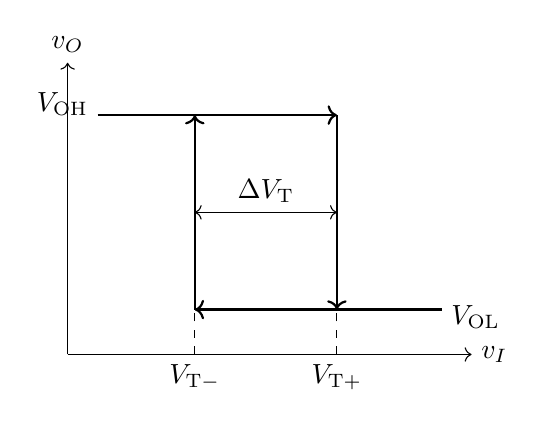
\begin{tikzpicture}[scale=0.95]
    \draw[->] (0,0) -- (5.4,0) node[right] {$v_I$};
    \draw[->] (0,0) -- (0,3.9) node[above] {$v_O$};
    % 滞回环：上支为 vI 增大时的路径，下支为 vI 减小时的路径
    \draw[thick,->] (0.4,3.2) -- (3.6,3.2);
    \draw[thick,->] (3.6,3.2) -- (3.6,0.6);
    \draw[thick,->] (5.0,0.6) -- (1.7,0.6);
    \draw[thick,->] (1.7,0.6) -- (1.7,3.2);
    \draw[dashed] (3.6,0) -- (3.6,0.6);
    \draw[dashed] (1.7,0) -- (1.7,0.6);
    \node[below] at (1.7,0) {$V_{\text{T}-}$};
    \node[below] at (3.6,0) {$V_{\text{T}+}$};
    \node[left] at (0.4,3.35) {$V_\text{OH}$};
    \node[right] at (5.0,0.5) {$V_\text{OL}$};
    \draw[<->] (1.7,1.9) -- (3.6,1.9);
    \node[above] at (2.65,1.9) {$\Delta V_\text{T}$};
\end{tikzpicture}
\caption{施密特触发器的电压传输特性（反相输出，箭头为 $v_I$ 变化方向）}
\end{figure}

\textbf{易错点}：两式只差一个符号，判据是"翻转前 $v_O$ 是什么电平"——$v_I$ 上升时翻转前 $v_O$ 为低电平，
反馈项使 $v_A$ 偏小，$v_I$ 必须更大，故 $V_{\text{T}+}$ 用 $1+R_1/R_2$；$v_I$ 下降时翻转前 $v_O$ 为高电平，
反馈项抬高 $v_A$，$v_I$ 可以更小，故 $V_{\text{T}-}$ 用 $1-R_1/R_2$。

\subsection{集成施密特触发器 7413}
7413 是 TTL 集成施密特触发器（双 4 输入与非门），内部四部分各有针对性：
\begin{enumerate}
    \item 输入级加"与门"，扩展输入端的逻辑功能；
    \item 施密特核心电路（正反馈回路），提供回差与陡峭边沿；
    \item 电平偏移电路，解决分立电路中 $V_\text{OL}$ 偏高的缺点；
    \item 推拉式输出级，使 $V_\text{OL}\le0.5\,\mathrm{V}$ 达到标准逻辑低电平，并提高带负载能力。
\end{enumerate}

\subsection{主要特点与典型应用}
\paragraph{主要特点}
输入信号在上升和下降过程中状态转换的输入电平不同（存在回差 $\Delta V_\text{T}$）；
状态转换时有正反馈，输出波形边沿变陡，与输入边沿陡缓无关；输入落在回差带内时输出保持原态，故抗噪声能力强。

\paragraph{典型应用}
\begin{enumerate}
    \item \textbf{波形变换}：把边沿缓慢的周期性信号（正弦、三角波）变为边沿很陡的矩形脉冲；
    \item \textbf{脉冲整形}：信号经长传输线（电容大、阻抗不匹配）或叠加噪声后变形，整形后得到理想波形；
    \item \textbf{脉冲鉴幅}：把幅度不同的脉冲序列中幅度大于 $V_{\text{T}+}$ 的脉冲鉴别出来，小于者被抑制。
\end{enumerate}

\section{单稳态触发器}
\subsection{电路特点}
\begin{enumerate}
    \item 有一个\textbf{稳态}和一个\textbf{暂稳态}；
    \item 在外界触发信号作用下由稳态翻到暂稳态，维持一段时间后\textbf{自动}返回稳态；
    \item 暂稳态时间只取决于\textbf{电路内部参数}（$R$、$C$），与触发脉冲的宽度、幅度无关。
\end{enumerate}
暂稳态靠 $RC$ 充放电维持，按 $RC$ 接法不同分为\textbf{微分型}与\textbf{积分型}。

\subsection{微分型单稳态触发器}
\paragraph{电路组成}
由 CMOS 门 $G_1$、$G_2$，输入端 $R_d$、$C_d$ 微分电路，以及接在 $G_1$ 输出与 $G_2$ 输入之间的 $R$、$C$ 定时电路组成。
设 $V_\text{OH}\approx V_\text{DD}$、$V_\text{OL}\approx0$、$V_\text{TH}\approx V_\text{DD}/2$。

\paragraph{工作过程}
\textbf{稳态}：无触发时 $v_I=0$、$v_{I2}=V_\text{DD}$，故 $v_O=0$、$v_{O1}=V_\text{DD}$，电容无电压 $v_C=0$。\\
\textbf{触发}：$v_I$ 加触发脉冲，$R_d$、$C_d$ 微分后得到很窄的正负尖峰 $v_d$；$v_d$ 升到 $V_\text{TH}$ 后产生正反馈
$v_d\uparrow\rightarrow v_{O1}\downarrow\rightarrow v_{I2}\downarrow\rightarrow v_O\uparrow$，
$v_{O1}$ 跳为低电平，电容电压不能跃变故 $v_{I2}$ 同时为低电平，$v_O$ 翻为高电平，进入暂稳态。\\
\textbf{返回}：暂稳态中 $V_\text{DD}$ 经 $R$ 和 $G_1$ 输出电路给 $C$ 充电，$v_{I2}$ 指数上升；到 $v_{I2}=V_\text{TH}$ 时又一次正反馈，
$v_{O1}$、$v_{I2}$ 跳回高电平，$v_O$ 回 0；随后 $C$ 经 $R$ 与 $G_2$ 输入保护电路迅速放电到 0，电路完全恢复。

\paragraph{脉冲宽度}
充电起始值 $v_C(0)=0$、终了值 $v_C(\infty)=V_\text{DD}$、转换值 $v_C(t_\text{W})=V_\text{TH}$，代入三要素公式
\[
t_\text{W}=\tau\ln\frac{v_C(\infty)-v_C(0)}{v_C(\infty)-v_C(t_\text{W})}
=RC\ln\frac{V_\text{DD}}{V_\text{DD}-V_\text{TH}}=RC\ln2\approx0.69RC
\]
严格写 $\tau\approx(R+R_\text{ON})C$，$R_\text{ON}$ 为 $G_1$ 导通时的输出电阻。

\paragraph{其余参数}
\[
T_\text{re}\approx(3\sim5)R_\text{ON}C,\qquad T_\text{d}=t_\text{W}+T_\text{re},\qquad V_\text{m}=V_\text{OH}-V_\text{OL}\approx V_\text{DD}
\]
$T_\text{re}$ 为恢复时间（经验公式），$T_\text{d}$ 为分辨时间，即相邻两次触发的最小间隔；脉冲周期取决于输入触发脉冲周期。
本电路可用窄脉冲触发，但输出脉冲的下降沿较差。

\subsection{积分型单稳态触发器}
\paragraph{电路组成与工作过程}
由 TTL 与非门、反相器和 $RC$ 积分电路组成，用\textbf{正脉冲}触发。
$v_I=0$ 为稳态，$v_{O1}=V_\text{OH}$ 经 $R$ 很快把 $C$ 充到 $v_A=V_\text{OH}$（$R$ 较小）。
$v_I$ 变高后 $v_{O1}=V_\text{OL}$，电容电压不能突变，$v_A$ 仍为高电平，$v_O=V_\text{OL}$，进入暂稳态，$C$ 经 $R$ 放电；
$v_A$ 降到 $G_2$ 开启电压 $V_\text{TH}$ 时输出翻回高电平，回到稳态；$v_I$ 回低电平后 $v_{O1}$ 重新为高并向 $C$ 充电。

\paragraph{脉冲宽度}
\[
t_\text{W}=(R+R_\text{O})C\ln\frac{V_\text{OL}-V_\text{OH}}{V_\text{OL}-V_\text{TH}}
\]
$R_\text{O}$ 为 $G_1$ 输出低电平时的输出电阻。

\subsection{两种单稳态触发器的比较}
\begin{table}[htbp]
\centering
\caption{微分型与积分型单稳态触发器的比较}
\begin{tabular}{lll}
\toprule
比较项 & 微分型 & 积分型 \\
\midrule
$RC$ 电路位置 & 门间耦合（微分） & $G_2$ 输入端（积分） \\
有无正反馈 & 有 & 无 \\
输出边沿 & 前后沿都比较陡 & 边沿较差 \\
抗干扰能力 & 差 & 强 \\
对触发脉冲的要求 & 可用窄脉冲（宽度小于 $t_\text{W}$） & 触发脉冲宽度必须大于 $t_\text{W}$ \\
\bottomrule
\end{tabular}
\end{table}

\subsection{集成单稳态触发器 74121}
\paragraph{引脚与触发方式}
$\overline{A_1}$、$\overline{A_2}$ 为\textbf{下降沿}触发端（两者至少一个接低电平），$B$ 为\textbf{上升沿}触发端；
片内设 $R_\text{int}\approx2\,\mathrm{k}\Omega$ 内部定时电阻可代替外接电阻，也可外接 $R_\text{ext}$、$C_\text{ext}$ 自行设定脉宽。

\paragraph{脉宽计算与范围}
\[
t_\text{W}=0.69R_\text{ext}C_\text{ext}
\]
课件适用范围：$R_\text{ext}=2\,\mathrm{k}\Omega\sim30\,\mathrm{k}\Omega$、$C_\text{ext}=10\,\mathrm{pF}\sim10\,\mu\mathrm{F}$，
对应 $t_\text{W}=20\,\mathrm{ns}\sim200\,\mathrm{ms}$。$R_\text{ext}$ 过小会损坏芯片，过大会因漏电流引入误差。

\paragraph{不可重复触发与可重复触发}
\textbf{不可重复触发型}：进入暂稳态后再加触发脉冲不影响工作过程，必须待暂稳态结束才能接受下一个触发，
74121、74221、74LS221 属此类；\textbf{可重复触发型}：暂稳态期间再次触发会重新计时，输出脉冲再延续一个 $t_\text{W}$
（脉宽被展宽），74122、74LS122、74123、74LS123 属此类；部分型号（74221、74122、74123）另设复位端可提前结束暂稳态。

\paragraph{应用}
\textbf{定时}：产生固定宽度的选通脉冲，宽度由 $R$、$C$ 精确设定而与输入无关；\textbf{整形}：把不规则输入整形成规范的宽度与幅度；
\textbf{延时}：用两级单稳的脉宽差实现脉冲延时输出。

\section{多谐振荡器}
\subsection{自激振荡的条件与分类}
多谐振荡器是\textbf{自激振荡器}，接通电源后不需外加触发信号即自动产生矩形脉冲；因矩形波含丰富高次谐波而得名（又称无稳态电路）。
自激振荡的必要条件是电路\textbf{没有稳定状态}，实现办法有两类：
\begin{enumerate}
    \item 让门电路静态时工作在电压传输特性的\textbf{转折区}（放大状态），任何微小扰动都被正反馈放大而振荡——对称式、非对称式；
    \item 利用\textbf{延迟负反馈}（门电路传输延迟加 $RC$ 延时）形成振荡——环形振荡器。
\end{enumerate}

\subsection{对称式多谐振荡器}
\paragraph{电路结构与静态工作点}
两反相器 $G_1$、$G_2$ 经耦合电容 $C_1$、$C_2$ 接成正反馈回路，并在各管输入与输出间跨接 $R_{F1}$、$R_{F2}$，
把静态工作点偏置到电压传输特性的转折区。忽略门输出电阻，由叠加定理得反馈电阻在输入端引入的电压
\[
v_I=\frac{R_F}{R_1+R_F}V_\text{CC}+\frac{R_1}{R_1+R_F}v_O
\]
该直线与电压传输特性的交点即静态工作点 $P$；只要 $P$ 落在转折区（电压放大倍数大于 1），电路必然振荡。
对 74 系列门，$R_F$ 约取 $0.5\sim1.9\,\mathrm{k}\Omega$。

\paragraph{振荡过程与周期}
扰动使 $v_{I1}$ 微升，经两级正反馈后 $v_{O1}$ 变低、$v_{O2}$ 变高，进入第一个暂稳态，同时 $C_1$ 充电、$C_2$ 放电；
$C_1$ 同时经 $R_1$ 与 $R_{F2}$ 两条支路充电，充电较快，$v_{I2}$ 先升到 $V_\text{TH}$，又触发一次正反馈，进入第二个暂稳态，如此往复。
把 $C_1$ 充电回路用戴维宁定理等效得 $R_{\text{E}1}=\dfrac{R_1R_{F2}}{R_1+R_{F2}}$、
$V_{\text{E}1}=V_\text{OH}+\dfrac{R_{F2}}{R_1+R_{F2}}\left(V_\text{CC}-V_\text{OH}-V_\text{BE}\right)$；
考虑 TTL 输入钳位二极管，负跳变只能下跳到 $V_\text{IK}$，故 $v_C(0)=V_\text{IK}$、$v_C(\infty)=V_{\text{E}1}$、$v_C(t)=V_\text{TH}$：
\[
T_1=R_{\text{E}1}C_1\ln\frac{V_{\text{E}1}-V_\text{IK}}{V_{\text{E}1}-V_\text{TH}},
\qquad
T=2T_1=2R_\text{E}C\ln\frac{V_\text{E}-V_\text{IK}}{V_\text{E}-V_\text{TH}}
\]
若为 74LS 系列（$V_\text{OH}=3.4\,\mathrm{V}$、$V_\text{IK}=-1\,\mathrm{V}$、$V_\text{TH}=1.1\,\mathrm{V}$）且 $R_F\ll R_1$，可简化为
\[
T\approx2R_FC\ln\frac{V_\text{OH}-V_\text{IK}}{V_\text{OH}-V_\text{TH}}\approx1.3R_FC
\]

\subsection{非对称式多谐振荡器}
\paragraph{简化思路}
对称式电路中 $G_1$ 静态时工作在转折区，其输出电压本身就是界于高、低电平之间的偏置电压，直接接到 $G_2$ 输入端
即可使 $G_2$ 的静态工作点也落在转折区，因此可去掉 $C_2$ 与 $R_{F2}$，只在反馈回路保留一只电容 $C$ 与电阻 $R_F$。

\paragraph{静态工作点与周期}
以 CMOS 反相器为例，$R_F$ 跨接在 $G_1$ 输入与输出间且 $G_1$ 输入电流近似为零，故 $v_{O1}=v_{I1}$，
该直线与电压传输特性的交点即静态工作点，又因 $v_{I2}=v_{O1}$，$G_2$ 的静态工作点也在特性中点；流过 $R_F$ 的静态电流近似为零，对 $R_F$ 阻值无严格限制。
设 $G_2$ 输入保护电阻 $R_S$ 足够大、$R_F$ 远大于门导通电阻，则
$T_1\approx R_FC\ln\dfrac{V_\text{DD}-V_{\text{T}-}}{V_\text{DD}-V_{\text{T}+}}\approx R_FC\ln3$，放电时间同理，故
\[
T=T_1+T_2=2R_FC\ln3\approx2.2R_FC
\]
这是本章出现频率最高的多谐振荡周期公式，务必记住系数 $2.2$ 与 $\ln3$。

\subsection{环形振荡器}
把奇数个（$n\ge3$）反相器首尾相连构成闭合回路，利用门电路\textbf{传输延迟时间}形成延迟负反馈即产生自激振荡。
静态时任一门的输入、输出都不可能稳定在高、低电平，只能处于放大状态，故电路无稳定状态；
扰动经 $n$ 级延迟 $n\,t_\text{pd}$ 反相回到起点，再经 $n\,t_\text{pd}$ 又反相一次，如此往复：
\[
T=2n\,t_\text{pd}
\]
$n$ 为串联反相器个数（奇数），$t_\text{pd}$ 为单级门平均传输延迟时间。
门电路延迟极短（TTL 几十纳秒、CMOS 一二百纳秒），基本环形电路频率高且不易调节；
实用电路在回路中串入 $RC$ 延迟环节（并在 $G_1$ 输入端加保护电阻），使周期主要由 $RC$ 决定、频率可连续调节。

\subsection{用施密特触发器构成的多谐振荡器}
\paragraph{工作原理}
施密特反相器输出经 $R$ 反馈到输入端，输入端再经 $C$ 接地。设通电时 $v_I=0$、$v_O=V_\text{OH}$，
$V_\text{OH}$ 经 $R$ 向 $C$ 充电使 $v_I$ 上升；到 $V_{\text{T}+}$ 时输出翻为 $V_\text{OL}$，$C$ 经 $R$ 放电使 $v_I$ 下降；
降到 $V_{\text{T}-}$ 时又翻回高电平，在 $V_{\text{T}-}$ 与 $V_{\text{T}+}$ 之间往复振荡。

\paragraph{振荡周期与占空比调节}
设 CMOS 施密特触发器 $V_\text{OL}\approx0$、$V_\text{OH}\approx V_\text{DD}$，则
\[
T=RC\ln\left(\frac{V_\text{DD}-V_{\text{T}-}}{V_\text{DD}-V_{\text{T}+}}\cdot\frac{V_{\text{T}+}}{V_{\text{T}-}}\right)
\]
第一项对应充电时间、第二项对应放电时间。基本电路占空比不可调；
若在充电、放电支路各串一只方向相反的二极管，使充电只经 $R_2$、放电只经 $R_1$，则
\[
T=T_1+T_2\approx R_2C\ln\frac{V_\text{DD}-V_{\text{T}-}}{V_\text{DD}-V_{\text{T}+}}
+R_1C\ln\frac{V_{\text{T}+}}{V_{\text{T}-}}
\]
改变 $R_1$、$R_2$ 的比值即可改变占空比。

\subsection{石英晶体多谐振荡器}
石英晶体在固有谐振频率 $f_0$ 处阻抗最小（接近纯电阻）、相移为零，满足振荡的相位条件；偏离 $f_0$ 时阻抗迅速增大，
正反馈不足以维持振荡。故把晶体串入反馈回路后，\textbf{振荡频率只取决于晶体的固有谐振频率}，与 $R$、$C$ 及电源电压几乎无关。
典型电路用反相器配晶体与两只约 $30\,\mathrm{pF}$ 的匹配电容，频率稳定度可达 $10^{-5}\sim10^{-6}$ 量级，
远高于 $RC$ 型多谐振荡器（约 $10^{-1}\sim10^{-2}$），常用于时钟基准与时基电路。
晶体既可接在对称式、也可接在非对称式多谐振荡电路中，两者振荡频率都由晶体决定，$RC$ 只影响起振与输出波形。

\section{555 定时器及其应用}
\subsection{电路结构与功能表}
\paragraph{内部组成}
555 是数/模混合集成电路，由五部分组成：
\begin{enumerate}
    \item 三个 $5\,\mathrm{k}\Omega$ 电阻构成分压器，为比较器提供 $\frac{2}{3}V_\text{CC}$ 与 $\frac{1}{3}V_\text{CC}$ 的参考电压；
    \item 电压比较器 $C_1$、$C_2$：$C_1$ 反相端接高电平触发端 TH（6 脚）、同相端接 $\frac{2}{3}V_\text{CC}$；
    $C_2$ 同相端接低电平触发端 $\overline{\text{TR}}$（2 脚）、反相端接 $\frac{1}{3}V_\text{CC}$；
    \item SR 锁存器，把两比较器输出锁存为 $Q$、$\overline{Q}$；
    \item 输出缓冲器 $G$，输出端（3 脚）电流可达 $200\,\mathrm{mA}$；
    \item 放电三极管 $T_D$（OC 输出管），受 $\overline{Q}$ 控制，$Q=0$ 时导通，外接电容经 7 脚放电。
\end{enumerate}

\paragraph{功能表}
\begin{table}[htbp]
\centering
\caption{555 定时器的功能表（CB555）}
\begin{tabular}{ccccc}
\toprule
$\overline{R_D}$ & $v_{I1}$（TH，6 脚） & $v_{I2}$（$\overline{\text{TR}}$，2 脚） & $v_O$ & $T_D$ \\
\midrule
0 & $\times$ & $\times$ & 低 & 导通 \\
1 & $>\frac{2}{3}V_\text{CC}$ & $>\frac{1}{3}V_\text{CC}$ & 低 & 导通 \\
1 & $<\frac{2}{3}V_\text{CC}$ & $>\frac{1}{3}V_\text{CC}$ & 不变 & 不变 \\
1 & $<\frac{2}{3}V_\text{CC}$ & $<\frac{1}{3}V_\text{CC}$ & 高 & 截止 \\
1 & $>\frac{2}{3}V_\text{CC}$ & $<\frac{1}{3}V_\text{CC}$ & 高 & 截止 \\
\bottomrule
\end{tabular}
\end{table}
记忆口诀：\textbf{"都大为 0，都小为 1，一小一大是保持"}；$\overline{R_D}=0$ 时无条件复位。

\paragraph{各引脚功能}
1 脚接地 GND；2 脚低电平触发端（$v_{I2}<\frac{1}{3}V_\text{CC}$ 使 $Q=1$）；3 脚输出端（输出电压约比电源低 $1\sim3\,\mathrm{V}$，
可直接驱动继电器、LED、扬声器）；4 脚复位端 $\overline{R_D}$（输入负脉冲直接复位，不用时接高电平）；
5 脚电压控制端 $V_\text{CO}$（外加电压可改变比较器参考电压，不用时悬空或经 $0.01\,\mu\mathrm{F}$ 电容接地）；
6 脚高电平触发端 TH（$v_{I1}>\frac{2}{3}V_\text{CC}$ 使 $Q=0$）；7 脚放电端（$Q=0$ 时 $T_D$ 导通，外接电容经此放电）；
8 脚电源端（$5\sim18\,\mathrm{V}$）。

\subsection{接成施密特触发器}
\paragraph{接法与阈值}
2、6 脚短接作输入端，4、8 脚接电源，5 脚经 $0.01\,\mu\mathrm{F}$ 电容接地，7 脚悬空。
$v_I$ 升高：$v_I<\frac{1}{3}V_\text{CC}$ 时 $Q=1$、$v_O=V_\text{OH}$；$\frac{1}{3}V_\text{CC}<v_I<\frac{2}{3}V_\text{CC}$ 时保持；
$v_I>\frac{2}{3}V_\text{CC}$ 时 $Q=0$、$v_O=V_\text{OL}$。故 $V_{\text{T}+}=\frac{2}{3}V_\text{CC}$。
$v_I$ 降低：$v_I<\frac{1}{3}V_\text{CC}$ 时 $Q=1$、$v_O=V_\text{OH}$。故 $V_{\text{T}-}=\frac{1}{3}V_\text{CC}$，回差 $\Delta V_\text{T}=\frac{1}{3}V_\text{CC}$。

\paragraph{回差可调}
若 5 脚由外电路提供 $V_\text{CO}$，则 $V_{\text{T}+}=V_\text{CO}$、$V_{\text{T}-}=\frac{1}{2}V_\text{CO}$、$\Delta V_\text{T}=\frac{1}{2}V_\text{CO}$，
改变 5 脚电压即可任意调节阈值与回差，这是 555 相对集成施密特触发器的优势。

\subsection{接成单稳态触发器}
\paragraph{接法与工作过程}
2 脚作触发输入，6、7 脚短接后接 $RC$ 定时回路（$R$ 接 $V_\text{CC}$、$C$ 接地），5 脚经 $0.01\,\mu\mathrm{F}$ 电容接地。
\textbf{稳态}：无触发时 $v_{I2}>\frac{1}{3}V_\text{CC}$，若通电后 $Q=0$，则 $T_D$ 导通、$C$ 经 7 脚放电到 $v_C=0$，
$v_{I1}=0<\frac{2}{3}V_\text{CC}$，锁存器保持 $Q=0$、$v_O=0$。
\textbf{暂稳态}：触发脉冲下降沿使 $v_{I2}<\frac{1}{3}V_\text{CC}$，锁存器置 1，$Q=1$、$v_O$ 跳高、$T_D$ 截止，
$V_\text{CC}$ 经 $R$ 给 $C$ 充电；$v_C$ 充到 $\frac{2}{3}V_\text{CC}$ 时 $C_1$ 使锁存器复位，$Q=0$、$v_O$ 回低、$T_D$ 导通，$C$ 迅速放电，恢复稳态。

\paragraph{脉宽计算}
充电起始值 $v_C(0)=0$、终了值 $v_C(\infty)=V_\text{CC}$、转换值 $v_C(t_\text{W})=\frac{2}{3}V_\text{CC}$：
\[
t_\text{W}=RC\ln\frac{V_\text{CC}-0}{V_\text{CC}-\frac{2}{3}V_\text{CC}}=RC\ln3\approx1.1RC
\]
\textbf{易错点}：555 单稳系数是 $1.1$（$\ln3$），门电路微分型单稳是 $0.69$（$\ln2$），不可混用；
差别源于充电的"目标值"不同——前者充到 $\frac{2}{3}V_\text{CC}$ 就翻转，后者充到 $\frac{1}{2}V_\text{DD}$ 就翻转。
此外触发脉冲宽度必须小于 $t_\text{W}$、幅度应低于 $\frac{1}{3}V_\text{CC}$，否则电路无法正常返回。

\subsection{接成多谐振荡器}
\paragraph{接法与工作过程}
2、6 脚短接后接电容 $C$ 上端（$C$ 下端接地）；7 脚接在 $R_1$、$R_2$ 之间，$R_1$ 另一端接 $V_\text{CC}$、$R_2$ 另一端接 2、6 脚。
设通电后 $Q=1$、$T_D$ 截止，$V_\text{CC}$ 经 $R_1$、$R_2$ 给 $C$ 充电，$v_C$ 上升；到 $\frac{2}{3}V_\text{CC}$ 时 $C_1$ 使锁存器复位，
$Q=0$、$T_D$ 导通，$C$ 经 $R_2$ 与 $T_D$ 放电，$v_C$ 下降；到 $\frac{1}{3}V_\text{CC}$ 时 $C_2$ 使锁存器置 1，$T_D$ 又截止，重新充电，
在 $\frac{1}{3}V_\text{CC}$ 与 $\frac{2}{3}V_\text{CC}$ 之间往复，输出连续矩形波。

\paragraph{周期与占空比}
\[
T_1=(R_1+R_2)C\ln2,\quad T_2=R_2C\ln2,\quad
T=(R_1+2R_2)C\ln2\approx0.69(R_1+2R_2)C
\]
\[
q=\frac{T_1}{T}=\frac{R_1+R_2}{R_1+2R_2}>50\%
\]
标准 555 多谐振荡器的占空比恒大于 50\%、不能小于 50\%，这是其固有缺点。

\paragraph{占空比可调的改进电路}
在 $R_1$、$R_2$ 支路各串一只方向相反的二极管，使充电只经 $R_\text{充}$、放电只经 $R_\text{放}$，则
\[
T_1=R_\text{充}C\ln2,\quad T_2=R_\text{放}C\ln2,\quad
T=(R_\text{充}+R_\text{放})C\ln2,\quad q=\frac{R_\text{充}}{R_\text{充}+R_\text{放}}
\]
选取不同的 $R_\text{充}$、$R_\text{放}$ 即可得到任意占空比（包括小于 50\%）。

\section{本章分析步骤与易错点}
\subsection{三类电路的分析步骤}
\begin{enumerate}
    \item \textbf{施密特触发器}：判断两个稳态（谁导通、$v_O$ 为何电平）→ 找翻转的临界条件（$v_A=V_\text{TH}$ 或 $v_I=v_\text{E}+0.7\,\mathrm{V}$）
    → 用叠加原理或分压关系解出 $V_{\text{T}+}$、$V_{\text{T}-}$ → 回差取两者之差。
    \item \textbf{单稳态触发器}：定稳态 → 定触发方式（上升沿/下降沿、哪一个端子）→ 定暂稳态由哪个 $RC$ 充放电维持
    → 用三要素公式求 $t_\text{W}$ → 校核恢复时间 $T_\text{re}$ 与分辨时间 $T_\text{d}$。
    \item \textbf{多谐振荡器}：找两个暂稳态的转换阈值 → 定每段充放电回路的等效电阻与等效电源 → 分别求 $T_1$、$T_2$
    → 相加得 $T$，占空比 $q=T_1/T$。
\end{enumerate}

\subsection{易错点清单}
\begin{itemize}
    \item $t_\text{W}=1.1RC$（$\ln3$）只属于"充到 $\frac{2}{3}V_\text{CC}$ 翻转"的场合（555 单稳、555 多谐的每一段）；
    门电路单稳与施密特型多谐的阈值是 $V_\text{TH}=V_\text{DD}/2$，对应 $\ln2\approx0.69$。
    \item 施密特触发器 $V_{\text{T}+}$、$V_{\text{T}-}$ 的反馈电平判断错，会导致回差符号反、甚至算出负回差。
    \item 555 的 5 脚接外参考 $V_\text{CO}$ 后，两个阈值变为 $V_\text{CO}$ 与 $V_\text{CO}/2$，不再是 $\frac{2}{3}V_\text{CC}$ 与 $\frac{1}{3}V_\text{CC}$。
    \item 标准 555 多谐振荡器的 $q$ 恒大于 50\%，不能靠改变 $R_1$、$R_2$ 的数值得到 $q<50\%$，必须改接二极管。
    \item 单稳态输出脉宽由 $R$、$C$ 决定而与触发脉冲无关；积分型单稳却要求触发脉冲宽度大于输出脉宽——
    这两句不矛盾：前者说"输出与输入无关"，后者说"电路正常工作的输入条件"。
\end{itemize}

\clearpage

% cSpell:ignore Schmitt,monostable,multivibrator,555,7413,74121,CMOS,TTL,VCC,LF398,ADC,DAC,CB7520,DAC0808,AD9012,AD9002,AD9020,ADC0804
\setlength{\parskip}{0.4em}
\setlength{\itemsep}{0.2em}
\setlength{\tabcolsep}{4pt}

\chapter{数一模和模一数转换}
\section{概述}
\subsection{应用用途}
计算机控制系统中，被控对象多为温度、压力、位移等非电量；传感器将非电量转为连续模拟量，经A/D转换得到数字量送入计算机运算处理；计算机输出数字量再经D/A转换还原模拟量，驱动执行机构调节被控对象。

\subsection{核心性能指标}
转换精度、转换速度是DAC与ADC两类转换器最关键性能指标。

\subsection{基本概念与分类}
1. \textbf{D/A转换器 DAC}
数字量向模拟量转换电路；主流类型：权电阻网络DAC、倒T形电阻网络DAC、权电流型DAC、权电容型DAC、开关树型DAC。
2. \textbf{A/D转换器 ADC}
模拟量向数字量转换电路；分为直接型ADC、间接型ADC；按输出格式分为并行输出ADC、串行输出ADC。
教材先讲解DAC，DAC电路原理更简单，也是ADC内部组成单元。

\section{D/A转换器}
\subsection{DAC整体结构框架}
完整n位DAC由五部分构成：\textbf{数码寄存器、模拟开关阵列、解码电阻网络、求和放大电路、基准电压源}。
数字量串行/并行存入寄存器，寄存器输出逐位驱动模拟开关，开关将对应权值电流送入求和放大器，叠加得到与输入数字量成正比的模拟输出。

\subsection{DAC分类体系}
1. 按解码网络结构：T型电阻DAC、倒T型电阻DAC、权电流DAC、权电阻DAC；
2. 按模拟开关类型：
    - CMOS开关型（功耗低，转换速度慢）；
    - 双极型电流开关型（转换速度快，包含ECL电流开关）。

\subsection{权电阻网络D/A转换器}
\subsubsection{二进制数字量权值表达}
n位二进制数 $D_n = d_{n-1}d_{n-2}\dots d_1d_0 = 2^{n-1}d_{n-1}+2^{n-2}d_{n-2}+\dots+2^1d_1+2^0d_0$
$2^{n-1}$ 为最高位MSB权值，$2^0$ 为最低位LSB权值。

\subsubsection{电路组成}
4位权电阻DAC由：权电阻网络、四路模拟开关、求和运算放大器、基准电压$V_\text{REF}$组成。
开关逻辑：$d_i=1$ 开关接$V_\text{REF}$产生支路电流；$d_i=0$ 开关接地，支路电流为0。
支路权电流（4位）：
\[
I_3=\frac{V_\text{REF}}{R},\; I_2=\frac{V_\text{REF}}{2R},\; I_1=\frac{V_\text{REF}}{4R},\; I_0=\frac{V_\text{REF}}{8R}
\]

\subsubsection{运放虚短虚断基础}
深度负反馈运放线性区满足：虚短 $V_+=V_-=0$；虚断输入电流为0；反相比例输出 $v_O = -\frac{R_f}{R_1}U_1$。

\subsubsection{输出电压推导（取$R_f=R/2$）}
总求和电流 $i_\Sigma = I_3+I_2+I_1+I_0$
\[
\begin{aligned}
v_O &= -R_f i_\Sigma
= -\frac{R}{2}\left( \frac{V_\text{REF}}{R}d_3+\frac{V_\text{REF}}{2R}d_2+\frac{V_\text{REF}}{4R}d_1+\frac{V_\text{REF}}{8R}d_0 \right) \\
&= -\frac{V_\text{REF}}{2^4}\left(2^3d_3+2^2d_2+2^1d_1+2^0d_0\right)
\end{aligned}
\]
通用n位公式：
\[
v_O = -\frac{V_\text{REF}}{2^n} D_n
\]
输入全0时$v_O=0$；输入全1时 $v_O=-\frac{2^n-1}{2^n}V_\text{REF}$，输出范围 $0 \sim -\frac{2^n-1}{2^n}V_\text{REF}$。

\subsubsection{优缺点}
优点：电路结构简单、元件数量少；
缺点：各位电阻阻值相差极大，位数越多阻值差距越大，高精度电阻生产困难。

\subsection{倒T形电阻网络D/A转换器}
\subsubsection{设计目的}
解决权电阻DAC电阻值差异过大、精度难以保证的缺陷，仅使用$R、2R$两种电阻。

\subsubsection{电路电流特性}
利用虚地 $V_- \approx V_+=0$，无论开关接运放输入端还是地，每条2R支路流过电流恒定，从MSB到LSB电流逐次二分。
总基准电流 $I=\frac{V_\text{REF}}{R}$。

\subsubsection{n位通用输出公式}
\[
v_O = -\frac{V_\text{REF}}{2^n}\left(2^{n-1}d_{n-1}+\dots+2^1d_1+2^0d_0\right)
= -\frac{V_\text{REF}}{2^n}D_n
\]
输出范围、比例关系与权电阻DAC完全一致；$V_\text{REF}$取负值可得到正向输出电压。

\subsubsection{集成DAC CB7520（AD7520）}
10位倒T型CMOS开关DAC，片内集成倒T型$R/2R$电阻网络，需要外接运算放大器；基准电压$V_\text{REF}$精度直接决定转换精度。
10位输出公式：
\[
v_O = -\frac{V_\text{REF}}{2^{10}} D_{10}
\]

\subsubsection{单极性输出外围电路}
可外接调零电阻、反馈调节电阻，调节运放增益改变满量程输出幅度；$R_{W3}$为运放调零电阻，$R_{W1}$调节放大比例，$R_{W2}$串联分压缩小输入基准电流。

\subsection{权电流型D/A转换器}
\subsubsection{改进思路}
权电阻、倒T型DAC开关导通压降会引入转换误差；权电流DAC采用恒流源支路，支路电流不受开关导通内阻压降影响，降低开关匹配要求。

\subsubsection{电路原理}
恒流源支路电流仅由发射极回路参数固定，数字位$d_i=1$恒流源接入运放求和端，$d_i=0$接地；搭配倒T型电阻网络减少电阻种类。

\subsubsection{典型集成芯片 DAC0808}
8位双极型电流开关DAC，转换速度高；内置恒流基准电路，外部仅需运放、补偿电容、基准电压。

\subsection{双极性输出D/A转换器}
数字量包含正负符号（补码），需要DAC输出正负模拟电压；在单极性倒T型DAC求和端叠加偏移基准电流，偏移电流大小等于最高位权电流，实现正负对称输出。

\subsection{DAC转换精度与转换速度}
\subsubsection{转换精度两大指标}
1. \textbf{分辨率（理论精度）}
表征DAC分辨输入微小数字变化的能力，总共有$2^n$个输出等级：
\[
\text{分辨率} = \frac{1}{2^n - 1}
\]
位数$n$越大分辨率越高，也可用可分辨最小电压与满量程比值表示。

2. \textbf{转换误差（实际精度）}
实际输出与理想理论值的最大偏差，由基准源漂移、运放零点、开关内阻、电阻失配、器件非线性共同导致；分为三类：
    a) 比例系数误差：基准电压$V_\text{REF}$偏移带来，误差与输入数字成正比；
    b) 失调误差（平移误差）：运放零点漂移，整条转换曲线整体上下平移，与输入数字无关；
    c) 非线性误差：开关导通电阻、电阻失配引起，误差无固定线性规律；
总误差为各类误差绝对值叠加。

\subsubsection{转换速度——建立时间$t_\text{set}$}
数字输入突变后，输出模拟量进入稳态误差$\pm\frac{1}{2}\text{LSB}$区间所需时长；数字跳变幅度越大建立时间越长。
不含运放DAC：$t_\text{set}<0.1\mu\text{s}$；集成运放DAC：$t_\text{set}>1.5\mu\text{s}$；高速系统选用高速运放缩短建立时间。

\section{A/D转换器}
\subsection{A/D转换完整流程与前置单元}
\subsubsection{四大核心步骤}
连续模拟量转换为离散数字量，必须依次完成\textbf{取样、保持、量化、编码}四个环节，工程中取样和保持常集成在同一电路实现。

\subsubsection{取样定理（奈奎斯特采样定理）}
若输入模拟信号最高频率分量为$f_{i(\text{max})}$，取样频率$f_s$必须满足：
\[
f_s \ge 2f_{i(\text{max})}
\]
工程实用取值：$f_s=(3\sim5)f_{i(\text{max})}$；每次采样后必须保持采样电平稳定一段时间，为后续量化编码提供稳定输入。

\subsubsection{取样—保持电路}
1. \textbf{基础电路结构}
由运算放大器$\text{A}$、保持电容$C_H$、NMOS模拟开关$\text{T}$构成，$v_I$为模拟输入，$v_L$为取样控制时钟信号。
- 取样阶段（$v_L$高电平）：MOS管导通，输入电压通过$R_1$、导通管$\text{T}$向$C_H$充电，若取$R_1=R_f$且运放理想，则$v_O=v_C=-v_I$；
- 保持阶段（$v_L$低电平）：MOS管截止，电容$C_H$无放电回路，两端电压维持不变，输出锁定采样时刻电平；
保持电容漏电流越小、运放输入阻抗越高，保持时长越长。

2. \textbf{集成取样保持芯片LF398}
内部包含两级运放$\text{A}_1/\text{A}_2$、逻辑控制单元、模拟开关与保护二极管；$v_\text{OS}$为失调调零端，可外接电阻修正输出零点；二极管$D_1/D_2$用于过压保护，避免开关单元承受过高电压。

\subsubsection{量化与编码}
1. \textbf{量化定义}
将连续模拟电压划分成多个离散等级，每一级最小电压间隔称为量化单位$\Delta$（对应数字量最低位LSB），所有采样电压归并到最近的量化等级，该过程会引入固有量化误差。
2. \textbf{两种量化方式}
- \textbf{只舍不入量化}：不足一个量化单位的部分全部舍去，最大量化误差为$\Delta$；
- \textbf{四舍五入量化}：小于半个量化单位舍去、大于等于半个量化单位向上取整，最大量化误差仅$\Delta/2$，工业ADC普遍采用该方案。
3. \textbf{编码}
将量化后的离散电平用二进制（或其他进制）代码表示，最终输出标准数字信号；正负范围输入多采用二进制补码编码。

\subsubsection{ADC整体分类框架}
\begin{itemize}
\item 直接型ADC：并联比较型、反馈比较型（计数型、逐次渐近型）；
\item 间接型ADC：V-T变换型（单积分、双积分、四积分）、V-F变换型；
\end{itemize}

\subsection{直接型A/D转换器}
\subsubsection{并联比较型ADC}
1. \textbf{电路组成}
由分压电阻链、电压比较器组、寄存器、代码转换逻辑三部分构成，属于高速并行直接ADC。
2. \textbf{量化规则}
满量程$0\sim V_\text{REF}$范围内，$n$位ADC量化单位：
\[
\Delta=\frac{2V_\text{REF}}{2^{n+1}}
\]
比较器根据输入电平输出高低电平，经寄存器锁存后由组合逻辑转换为标准二进制输出。
3. \textbf{核心优缺点}
优点：转换速度极快，单次转换仅需几十纳秒，自带采样保持能力；
缺点：硬件开销极大，$n$位需要$2^n-1$个比较器与触发器，位数提升后硬件规模指数增长；转换精度由分压电阻、参考源精度决定。
4. \textbf{典型产品}
AD9012（8位TTL工艺）、AD9002（8位ECL工艺）、AD9020（10位TTL工艺）。

\subsubsection{反馈比较型ADC}
核心原理：将内部DAC输出的模拟电压和输入模拟电压对比，不断调整DAC输入数字量，直到二者逼近相等，最终数字量即为转换结果。
1. \textbf{计数型ADC}
由比较器、DAC、计数器、脉冲源、门控逻辑、输出寄存器组成：
- 清零后计数器从0开始逐脉冲累加，DAC输出阶梯电压逐步抬升；
- 当DAC输出超过输入电压时比较器翻转，关闭时钟门控，计数器数值锁存输出；
缺点：最长转换时长为$(2^n-1)T_{CP}$，速度很慢，仅适合低速场景。

2. \textbf{逐次渐近型ADC}
借鉴天平称重思路，从最高位到最低位逐位试探、逐位锁定，$n$位ADC仅需$n$次比较即可完成转换：
- 先将寄存器最高位置1，后续位清零，DAC输出试探电压和输入对比；
- 若DAC输出小于输入则保留该位1，否则清零，依次试探所有位；
优点：硬件规模远小于并联型、速度远快于计数型，是工业最通用的ADC架构。

\subsection{间接型A/D转换器——双积分型ADC}
\subsubsection{电路组成}
包含积分器、电压比较器、计数器、时序逻辑控制、时钟脉冲源五大模块，属于V-T变换型ADC。
\subsubsection{两步积分工作流程}
1. \textbf{第一次定时采样积分}：固定时长$T_1$对输入模拟电压$v_I$积分，积分输出：
\[
v_O=-\frac{T_1}{RC}v_I
\]
2. \textbf{第二次反向基准积分}：切换对固定负基准电压$-V_\text{REF}$积分，积分器从负电压往零回落，记录回落至0的时长$T_2$，满足：
\[
\frac{T_1}{RC}v_I=\frac{T_2}{RC}V_\text{REF} \implies T_2=\frac{T_1}{V_\text{REF}}v_I
\]
最终计数结果$D=\frac{T_2}{T_C}=\frac{2^n}{V_\text{REF}}v_I$，数字量和输入电压严格成正比。
\subsubsection{优缺点}
优点：抗工频干扰能力极强、对RC参数和时钟频率稳定性要求低、温漂小、转换精度极高；
缺点：转换速度慢，每秒仅能完成几十次转换，适合工业低速精密测量场景。
\subsubsection{典型集成芯片}
ADC-EK8B（8位二进制）、ADC-EK10B（10位二进制）、MC14433（$3\frac{1}{2}$位BCD码）、CB7106/CB7107（数码管驱动专用）。

\subsection{V-F变换型ADC}
先把模拟电压转换成与之成正比的脉冲频率，再在固定时间窗口内对频率脉冲计数，计数结果即为对应数字量；抗干扰性能优秀，适合远距离遥测场景。

\subsection{A/D转换器性能指标}
\subsubsection{分辨率}
用输出二进制/十进制位数表征，$n$位二进制ADC可区分$2^n$级输入电压，能分辨的最小输入电压为满量程的$\frac{1}{2^n}$，位数越高分辨率越强。
\subsubsection{转换误差}
实际输出数字量和理论理想值的最大偏差，工程要求误差不超过$\pm\frac{1}{2}\text{LSB}$；提升分辨率不能直接提高精度，必须让转换误差小于量化误差上限。
\subsubsection{转换速度}
用单次转换时间衡量：并联比较型速度最快、逐次渐近型次之、双积分间接型最慢；选型需要综合系统速度、精度、输入范围、功耗等多维度需求。

\subsection{集成A/D转换器及其应用}
\subsubsection{ADC0804集成芯片详解}
1. \textbf{基础特性}
采用CMOS工艺制作的逐次渐近型8位ADC，转换时长$100\mu\text{s}$，输入模拟电压范围$0\sim5\mathrm{V}$，片内自带输出锁存寄存器，可直接对接微机CPU数据总线，无需额外接口逻辑。

2. \textbf{引脚功能定义}
\begin{itemize}
\item $\boldsymbol{CS}$：片选信号输入，低电平有效，有效时芯片被选中启动工作；
\item $\boldsymbol{RD}$：读信号输入，低电平有效，$\boldsymbol{CS}$与$\boldsymbol{RD}$同时为低可读取转换结果；
\item $\boldsymbol{WR}$：写信号输入，低电平有效，$\boldsymbol{CS}$与$\boldsymbol{WR}$同时为低启动模数转换；
\item $\boldsymbol{CLKR}$：内部时钟发生器外接电阻端；
\item $\boldsymbol{CLKIN}$：外部时钟脉冲输入端；
\item $\boldsymbol{INTR}$：转换结束中断输出，低电平有效，转换完成后自动拉低，可作为CPU中断请求信号；
\item $\boldsymbol{V_{IN+}、V_{IN-}}$：差分模拟电压输入端，可接入单极性或双极性模拟信号；
\item $\boldsymbol{AGND}$：模拟信号地；$\boldsymbol{DGND}$：数字信号地；
\item $\boldsymbol{V_{REF}/2}$：参考电压分压输入端；
\item $\boldsymbol{D_7\sim D_0}$：8位三态并行数字输出端，可直接挂载微机总线；
\item $\boldsymbol{V_{CC}}$：芯片电源供电端。
\end{itemize}

3. \textbf{工作时序规范}
\begin{itemize}
\item 启动转换：$\boldsymbol{CS}$与$\boldsymbol{WR}$同时拉低，上升沿后开始转换，$100\mu\text{s}$内完成模数转换，转换结束后$\boldsymbol{INTR}$自动变低；
\item 读取结果：$\boldsymbol{CS}$与$\boldsymbol{RD}$同时拉低，内部三态门打开，数据输出到总线；电平恢复高电平后三态门回到高阻态。
\end{itemize}

4. \textbf{使用关键注意事项}
\begin{itemize}
\item 接地设计：模拟地（AGND）与数字地（DGND）需要分别布线，仅在电源处单点共接，避免数字开关噪声干扰模拟前端；
\item 零点与满量程调节：通过配套引脚外接微调电阻，修正零点偏差和满量程输出偏差；
\item 参考电压调节：根据输入量程配置参考电压，保障转换线性度；
\item 总线时序配合：严格匹配微机读写时序，防止数据采样出错。
\end{itemize}

5. \textbf{典型应用架构}
可直接挂接微机系统控制总线，配合RAM实现数据缓存；模拟信号送入ADC0804完成转换后，数字量上传至微处理器控制器，实现多路采集、数据处理与外设联动控制。

\end{document}